\documentclass[graybox, envcountchap]{svmult}
% Springer document settings
\usepackage[bottom]{footmisc}% places footnotes at page bottom

\usepackage{newtxtext}       % 
\usepackage[varvw]{newtxmath}       % selects Times Roman as basic font
%%%%%%%%%%%%%%%%%%%%%%%%%%%%%%%

% \usepackage{amssymb}
\usepackage{ntheorem}
\usepackage{amsmath}
\usepackage{enumitem}


\usepackage{graphicx}
\usepackage{color}
\usepackage{cite}
\usepackage{makeidx}


\usepackage{ascmac}
\usepackage{eclbkbox}
\usepackage{dsfont}

\usepackage{longtable}

\usepackage{url}

\usepackage{hyperref}

\usepackage{multicol}

%% --川口追加--
\makeatletter
\let\MYcaption\@makecaption
\makeatother
\usepackage{subcaption}
\captionsetup{compatibility=false}      % 必要に応じて

\makeatletter
\let\@makecaption\MYcaption
\makeatother
% ----

%%
\theoremstyle{plain}
\theoremheaderfont{\bfseries}
\theorembodyfont{\rmfamily}
\theoremseparator{\hspace{1ex}}
\theoremindent0cm
\theoremnumbering{arabic}
\theoremprework{\vspace{1ex}\begin{shadebox}\vspace{1ex}}
\theorempostwork{\vspace{-1ex}\end{shadebox}\vspace{1ex}}

%%
\theoremclass{theorem}

%%
\theoremclass{theorem}

%%
\theoremclass{theorem}


%%
\theoremstyle{break}
\theoremheaderfont{\bfseries}
\theorembodyfont{\rmfamily}
\theoremseparator{}
\theoremindent0cm
\theoremnumbering{arabic}
\theoremprework{\vspace{1.5ex}\begin{breakbox}\vspace{-0.5ex}}
\theorempostwork{\vspace{-0.5ex}\end{breakbox}\vspace{1.5ex}}

%%
\theoremstyle{nonumberplain}
\theoremseparator{\hspace{1ex}}

%%
\newtheorem{assumption}{Assumption}[section]

%%
\renewcommand{\theproblem}{}

\renewcommand{\theremark}{}


\newcommand{\red}[1]{{\color{red}#1}}
\newcommand{\blue}[1]{{\color{blue}#1}}
\newcommand{\green}[1]{{\color{green}#1}}

\DeclareMathOperator*{\argmax}{arg\,max}

\newcommand{\bm}[1]{\boldsymbol{#1}}
\newcommand{\sfT}{\mathsf{T}}

\newcommand{\advanced}{$^{\ddag}$}

\DeclareMathOperator{\sfsin}{\mathsf{sin}}
\DeclareMathOperator{\sfcos}{\mathsf{cos}}
\DeclareMathOperator{\sftan}{\mathsf{tan}}
\DeclareMathOperator{\sfarctan}{\mathsf{arctan}}

\DeclareMathOperator{\sfdiag}{\mathsf{diag}}
\DeclareMathOperator{\sfcol}{\mathsf{col}}
\DeclareMathOperator{\sfdet}{\mathsf{det}}
\DeclareMathOperator{\sfadj}{\mathsf{adj}}
\DeclareMathOperator{\sftrace}{\mathsf{trace}}

\DeclareMathOperator{\real}{\mathsf{Re}}

\DeclareMathOperator{\sfker}{\mathsf{ker}}
\DeclareMathOperator{\sfim}{\mathsf{im}}

\DeclareMathOperator{\sfdim}{\mathsf{dim}}
\DeclareMathOperator{\sfspan}{\mathsf{span}}

\DeclareMathOperator{\sfint}{\mathsf{int}}

\DeclareMathOperator*{\sfmin}{\mathsf{min}}
\DeclareMathOperator*{\sfmax}{\mathsf{max}}
\DeclareMathOperator*{\sfsup}{\mathsf{sup}}

\DeclareMathOperator{\sfsat}{\mathsf{sat}}

\newcommand{\mat}[1]{\left[\: \begin{matrix} #1 \end{matrix} \:\right]}
\newcommand{\spliteq}[1]{\begin{split} #1 \end{split}}
\newcommand{\simode}[1]{\begin{cases}  \begin{split} #1 \end{split} \end{cases}}

\newcommand{\proofend}{\hfill \rule{2mm}{3mm}}

\newcommand{\Xti}{X_i'}
\newcommand{\Xsi}{X_i}

\newcommand{\Xtone}{X_1'}
\newcommand{\XtN}{X_N'}

\newcommand{\Xt}{X'}
\newcommand{\Xs}{X}

\newcommand{\taudi}{\tau_i}
\newcommand{\taud}{\tau}

\newcommand{\Cgi}{b_i}


\newcommand{\Ifd}{I_{\rm field} }

\newcommand{\matlab}{\textsc{Matlab} }





%% --川口追加--
\newcommand{\thshift}{\theta_{12}}
\newcommand{\thshiftb}{\theta_{32}}
\newcommand{\Ysa}{\bm y_{12}}
\newcommand{\bca}{c_{12}}
\newcommand{\Ysb}{\bm y_{32}}
\newcommand{\bcb}{c_{32}}
\newcommand{\bcij}{c_{ij}}
\newcommand{\Is}{{\bm I}_{12}' }
\newcommand{\im}{\bm j}
\newcommand{\tr}{{\sf T}}

%%%%%%%%%%%%%%%%%%%%%%%%% code lines %%%%%%%%%%%%%%%%%%%%%%%%%%%%%%%%%%%%%%%%%%
\usepackage{listings}
\usepackage{xcolor}
\renewcommand{\lstlistingname}{Program}% Listing -> Algorithm
\renewcommand{\lstlistlistingname}{List of \lstlistingname s}% List of Listings -> List of Algorithms

\definecolor{codegreen}{rgb}{0,0.6,0}
\definecolor{codegray}{rgb}{0.5,0.5,0.5}
\definecolor{codepurple}{rgb}{0.58,0,0.82}
\definecolor{backcolour}{rgb}{0.95,0.95,0.92}

\lstdefinestyle{mystyle}{
    backgroundcolor=\color{backcolour},   
    commentstyle=\color{codegreen},
    keywordstyle=\color{magenta},
    numberstyle=\tiny\color{codegray},
    stringstyle=\color{codepurple},
    basicstyle=\ttfamily\footnotesize,
    breakatwhitespace=false,         
    breaklines=true,                 
    captionpos=b,                    
    keepspaces=true,                 
    numbers=left,                    
    numbersep=5pt,                  
    showspaces=false,                
    showstringspaces=false,
    showtabs=false,                  
    tabsize=2
}

\lstset{style=mystyle}

\begin{document}

\chapter{Numerical simulation of the electrical power system
model}\label{chap:numcal}
In this chapter, we will explain numerical simulation methods for power system
models described by nonlinear differential algebraic equation systems. We will
also provide guidelines for building a structured numerical simulation
environment.

The chapter is organized as follows. First, in Section \ref{sec:howtocal}, we
will explain the difficulty of calculating the time response of power system
models. Next, in section \ref{sec:powflow}, we will describe the process of
power flow calculation, which numerically explores the equilibrium state of
power system models. In section \ref{sec:paradef}, we will discuss how to
determine the steady-state values of internal states of generators and constants
of load models that are consistent with the steady-state values of bus voltages
and power determined by power flow calculation.

In section \ref{sec:numsimtr}, we will explain the calculation methods for time
responses to changes in initial conditions, load fluctuations, and ground
faults, and illustrate the calculation of time responses. Finally, in section
\ref{sec:phsync}, we will discuss synchronism phenomena of bus voltages in
steady-state power flow states from an advanced perspective, and analyze them
mathematically.

\section{Calculation of time response of an electrical power
system}\label{sec:howtocal}

\subsection{Challenges in calculating time response}

In Chapter \ref{ch:model}, we explained that the mathematical model of the
entire power system, including generator and load models coupled with
transmission line models, is described by a system of nonlineadr differential
algebraic equations. Therefore, the time response of the power system model can
be obtained by numerically integrating these equations with appropriate initial
values and external inputs. However, when performing numerical simulations of
the power system model, it is necessary to consider specific characteristics of
the power system, such as:
\begin{itemize}
  \item If external inputs are not properly set, the demand and supply will not
  be in equilibrium, and the steady-state value of the frequency deviation will
  not be zero, causing the rotor angle of the generator to continue to change.
  \item There are an infinite number of combinations of external input values
  that result in zero steady-state value for frequency deviation. Therefore, it
  is necessary to specify realistic external input values.
  \item The values of the voltage phase and current phase of the bus bar group
  must be determined so that they are consistent as dependent variables with
  respect to the state variables of the generator group.
\end{itemize}

Therefore, simply using the differential-algebraic equation solver that is
standardly implemented in MATLAB is not sufficient to accurately execute
numerical simulations of the power system. This is one of the factors that makes
the calculation of the time response of the power system model difficult.

\subsection{Calculation steps}\label{sec:numstep}

The standard calculation procedure for the time response of a power system model
described by nonlinear differential algebraic equations is divided into the
following three steps:

\medskip
\begin{breakbox}
\begin{itemize}
  \item[(A)] To specify the power system state in a steady state where supply and
  demand are balanced, calculate the values of the phase angle and voltage of all
  buses in the steady state using the admittance matrix determined from the
  transmission network.
  \item[(B)] Calculate the steady-state values of the internal voltage and rotor
  angle of each generator, the external input values to the generator, and the
  impedance value of each load, so that they are consistent with the steady-state
  values of the bus current phase and voltage phase determined in Step A.
  \item[(C)] Using the power system state where supply and demand are balanced
  calculated in Steps A and B as the initial value, calculate the time response
  under various disturbances of different magnitudes such as giving perturbations
  to the internal state of the generator, grounding the voltage of the bus, or
  changing the parameter values of the load.
\end{itemize}
\end{breakbox}
\medskip

From the viewpoint of system control engineering, Step A can be understood as
"determining one equilibrium point to perform numerical analysis from among an
infinite number of equilibrium points." As described in Section
\ref{sec:paradef}, when the steady-state values of the phase angle and voltage
of all buses are given, there must exist steady-state values of the internal
state of the generator, external input values to the generator, and the load
parameter values that realize them. Therefore, calculating the steady-state
values of the phase angle and voltage of all buses is equivalent to calculating
the equilibrium point of the power system model represented by differential
algebraic equations. In power system engineering, this process is called the
\textbf{power flow calculation}\index{power flow calculation}. 

It should be noted that calculating the steady-state values of the internal
state of the generator, external input values, and the load parameter values in
Step B is an indirect procedure of determining the mathematical model of the
load from the results of the power flow calculation in Step A.  For example, if
you want to set the load connected to a certain bus as a constant impedance
model, you need to reverse calculate the impedance value of the load using the
current phase of the bus calculated by the power flow calculation divided by the
voltage phase.  If setting load model parameters as desired values, in Step C,
the time response to load parameter fluctuations is calculated while changing
the load parameters to desired values. 

Finally, in Step C, the time response of the electrical power system model is
calculated under various conditions depending on the purpose. For example, if
the external input to each generator and load parameter calculated in Steps A
and B are set as constants in the model, and the time response is calculated
with the initial value appropriate for generators, the internal state of the
generators asymptotically converges to the steady state calculated in Step B
over time. However, to set valid initial values such that asymptotic convergence
is established, as in Steps A and B, the equilibrium point that serves as the
reference for the analysis must be calculated first. The calculated equilibrium
point must be stable in an appropriate sense. 

\section{Numerical analysis of steady-state in power flow
calculation}\label{sec:powflow}

In this Section, we describe an overview of power flow calculation to
numerically search the steady-state of the power system, as explained in Step A
of Section \ref{sec:numstep} and the implementation method using MATLAB.

Given the admittance matrix $\bm{Y}$, the distribution of current and voltage
phasors of the busbar group that satisfies the following relationship is
referred to as the \textbf{power flow distribution} at time $t$.
\begin{equation}\label{eq:ohmY2}
\mat{
  \bm{I}_1(t)\\
  \vdots\\
  \bm{I}_N(t)
}
 =
\underbrace{
\mat{
  \bm{Y}_{11} & \cdots & \bm{Y}_{1N}\\
  \vdots & \ddots & \vdots\\
  \bm{Y}_{N1} & \cdots & \bm{Y}_{NN}
}
}_{\bm{Y}}
\mat{
  \bm{V}_1(t)\\
  \vdots\\
  \bm{V}_N(t)
}
\end{equation}

\begin{equation}\label{eq:pfconIV}
\bigl(
|\bm{I}_1(t)|,\angle \bm{I}_1(t),
|\bm{V}_1(t)|,\angle \bm{V}_1(t),
\ldots
|\bm{I}_N(t)|,\angle \bm{I}_N(t),
|\bm{V}_N(t)|,\angle \bm{V}_N(t)
\bigr)
\end{equation}

Each current and voltage phasors changes with time, and from the laws of physics
of current and voltage, these must satisfy Equation \ref{eq:ohmY2} at any
arbitrary time $t$. 

Power flow calculation is a computational process to find "one of the
steady-state power flow distributions". A steady-sate power flow distribution
refers to the condition that all the buses satisfy the following for given
constant current phasors $\bm{I}_i^{\star}$ and voltage phasors
$\bm{V}_i^{\star}$.

\[
  \bm{I}_i(t)=\bm{I}_i^{\star} ,\qquad
  \bm{V}_i(t)=\bm{V}_i^{\star}, \qquad
  \forall t\geq 0
\]

Using the definitions of active power and reactive power supplied to the bus
bars in the following equation, the current phasors can be eliminated.

\begin{align}\label{eq:defPQVIi2}
P_i(t)+\bm{j}Q_i(t) = \bm{V}_i(t) \overline{\bm{{I}} }_i(t)
\end{align}

Thus, the system of equations in Equation \ref{eq:ohmY2} is equilvalent to:

\begin{equation}\label{eq:PQVgen}
  \simode{
    P_1(t) + \bm{j} Q_1(t) &= 
    \sum_{j=1}^{N} \overline{\bm{Y}}_{1j} |\bm{V}_1(t)| |\bm{V}_j(t) | e^{\bm{j} \bigl(\angle \bm{V}_1(t) - \angle \bm{V}_j(t) \bigr)} \\ 
    & \; \;  \vdots \\
    P_N(t) + \bm{j} Q_N(t) &= 
    \sum_{j=1}^{N} \overline{\bm{Y}}_{Nj} |\bm{V}_N(t)| |\bm{V}_j(t) | e^{\bm{j} \bigl(\angle \bm{V}_N(t) - \angle \bm{V}_j(t) \bigr)}
  }
\end{equation}

Therefore, depending on the context, the distribution of active power, reactive
power, and voltage phasors satisfying Equation \ref{eq:PQVgen}  is referred to
as the power flow distribution at time $t$.

\begin{equation}\label{eq:pfcon}
  \bigl(
    P_1(t),Q_1(t),|\bm{V}_1(t)|,\angle \bm{V}_1(t),
    \ldots,
    P_N(t),Q_N(t),|\bm{V}_N(t)|,\angle \bm{V}_N(t)
  \bigr)
\end{equation}


\subsection{Outline of the power flow calculation}\label{sec:pfcal}

Let us explain the characteristics of the power flow calculation using a simple
example consisting of two bus bars.

\begin{figure}[t]
\centering
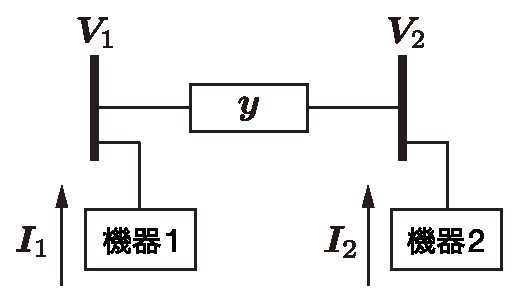
\includegraphics[width = .4\linewidth]{figs/2busex}
\medskip
\caption{\textbf{Power system model consisting of two bus bars}}
\label{fig:2buspf}
\medskip
\end{figure}

\begin{example}{\textbf{Power flow calculation of a two bus bar power system
model}}\label{ex:2buspf}

Let us consider an electrical power system consisting of two bus bars, as shown
in Figure \ref{fig:2buspf}.  We assume that each bus is connected to either a
load or a generator, but in power flow calculations, it is not necessary to
specify the type of device connected.

The admittance of a transmission line that connects two bus bars is denoted by
$\bm{y}\in \mathbb{C}$. When using the basic transmission line model, the
voltage and current phasors at the buses are related by:
\begin{equation}\label{eq:exyIV}
  \mat{
    \bm{I}_1^{\star}\\
    \bm{I}_2^{\star}
  }
  =
  \mat{
    \bm{y} & -\bm{y} \\
    -\bm{y} & \bm{y}
  }
  \mat{
    \bm{V}_1^{\star}\\
    \bm{V}_2^{\star}
  }
\end{equation}

However, to indicate that these values are in a steady-state, they are markeed
with a "${\star}$". Here, by eliminating the current phasors using the
relationship in Equation \ref{eq:defPQVIi2}, we obtain a system of equations
equivalent to Equation \ref{eq:exyIV} in terms of steady-state active power,
reactive power, and voltage phasors as follows:

\begin{subequations}\label{eq:PQpf}
\begin{equation}\label{eq:PQcom}
  \begin{aligned}
    P_1^{\star} + \bm{j} Q_1^{\star} &= 
    \overline{\bm{y}} \left( 
    |\bm{V}_1^{\star}|^2 
    -  |\bm{V}_1^{\star}| |\bm{V}_2^{\star}| e^{ \bm{j} (\angle \bm{V}_1^{\star}- \angle \bm{V}_2^{\star})}
    \right) \\
    P_2^{\star} + \bm{j} Q_2^{\star} &= 
    \overline{\bm{y}} \left( 
    |\bm{V}_2^{\star}|^2
    - |\bm{V}_1^{\star}| |\bm{V}_2^{\star}| e^{ \bm{j} (\angle \bm{V}_2^{\star} - \angle \bm{V}_1^{\star})}
    \right)
  \end{aligned}
\end{equation}

The objective of the power flow calculation is to determine the following set of
values that satisfy the above simultaneous equations. 

\[
(P_1^{\star},Q_1^{\star}, |\bm{V}_1^{\star}|, \angle \bm{V}_1^{\star}, P_2^{\star},Q_2^{\star},|\bm{V}_2^{\star}|, \angle \bm{V}_2^{\star})
\]

We denote the conductance and susceptance of a transmission line as:
\[
  g:= \operatorname{Re}[\bm{y}],\qquad
  b:= \operatorname{Im}[\bm{y}]
\]

Then, considering the real and imaginary parts of Equation \ref{eq:PQcom}, we
obtain a system of four equations:

\begin{equation}\label{eq:PQreal}
  \begin{aligned}
    P_1^{\star} &= g |\bm{V}_1^{\star}|^2  
    -   g |\bm{V}_1^{\star}| |\bm{V}_2^{\star}| \sfcos \angle \bm{V}_{12}^{\star}
    - b |\bm{V}_1^{\star}| |\bm{V}_2^{\star}| \sfsin \angle \bm{V}_{12}^{\star}
    \\
    P_2^{\star} &= g |\bm{V}_2^{\star}|^2  
    -  g |\bm{V}_1^{\star}| |\bm{V}_2^{\star}| \sfcos \angle \bm{V}_{21}^{\star}
    - b |\bm{V}_1^{\star}| |\bm{V}_2^{\star}| \sfsin \angle \bm{V}_{21}^{\star}
    \\
    Q_1^{\star} &= - b |\bm{V}_1^{\star}|^2  
    + b |\bm{V}_1^{\star}| |\bm{V}_2^{\star}| \sfcos \angle \bm{V}_{12}^{\star} 
    - g |\bm{V}_1^{\star}| |\bm{V}_2^{\star}| \sfsin \angle \bm{V}_{12}^{\star}
    \\
    Q_2 &= - b |\bm{V}_2^{\star}|^2  
    + b |\bm{V}_1^{\star}| |\bm{V}_2^{\star}| \sfcos \angle \bm{V}_{21}^{\star} 
    - g |\bm{V}_1^{\star}| |\bm{V}_2^{\star}| \sfsin \angle \bm{V}_{21}^{\star}
  \end{aligned}
\end{equation}
\end{subequations}
where $\angle \bm{V}_{ij}^{\star}$ represents $\angle \bm{V}_i^{\star}- \angle \bm{V}_j^{\star}$.

The phase of the voltage phasor is only meaningful in terms of the difference
value; thus, the number of variables that must be practically determined is
seven. Therefore, there are three variables of freedom in Equation
\ref{eq:PQreal}. To determine these, one can choose appropriate values for the
three variables $(|\bm{V}_1^{\star}|,|\bm{V}_2^{\star}|,\angle
\bm{V}_{12}^{\star})$. This allows us to calculate the remaining variables
$(P_1^{\star},P_2^{\star},Q_1^{\star},Q_2^{\star})$

However, with this method, while the voltage phase of each bus can be set to any
value, it is not possible to set the power supplied or consumed by each bus to
any value. That is, it is not possible to specify which bus is a load bus that
consumes power, or which bus is a generator bus that supplies power. Therefore,
in order to perform numerical simulations with realistic settings, it is often
necessary to properly determine the voltage phase values to achieve the
specified active and reactive power values.

For example, let us consider finding the
$(|\bm{V}_1^{\star}|,|\bm{V}_2^{\star}|,\angle \bm{V}_{12}^{\star})$ that
realize balanced active power supplied to the bus as:
\begin{equation}\label{eq:P1P2ex}
  P_1^{\star}=1,\qquad
  P_2^{\star}=-1
\end{equation}

This corresponds to determining the voltage phase distribution when the device
connected to bus 1 and bus 2 both supply and consume active power, respectively,
with both having a value of 1 in a steady-state condition. By adding the
equations in Equation \ref{eq:PQreal} with respect to $P_1^{\star}$ and
$P_2^{\star}$, we obtain:
\begin{equation*}
  \spliteq{
    0 &= g \Bigl\{
    |\bm{V}_1^{\star}|^2 + |\bm{V}_2^{\star}|^2 
    - 2 |\bm{V}_1^{\star}| |\bm{V}_2^{\star}| \sfcos \angle \bm{V}_{12}^{\star}
    \Bigr\}\\
    &=
    g \Bigl\{
    \left( |\bm{V}_1^{\star}| - |\bm{V}_2^{\star}| \right)^2 
    + 2 |\bm{V}_1^{\star}| |\bm{V}_2^{\star}| \bigl( 1-\sfcos \angle \bm{V}_{12}^{\star} \bigr)
    \Bigr\}
  }
\end{equation*}
Note that in realistic power flow conditions, the phase difference in voltage
phase between the buses, $\angle \bm{V}_{12}^{\star}$, is within the range of
$\pm \tfrac{\pi}{2}$. Moreover, it should be noted that if the phase angle
difference of the generator or the voltage phase difference of the bus exceeds
the range of $\pm \tfrac{\pi}{2}$, the slope of the sine function will be
inverted, resulting in an unrealistic transmission characteristic of active
power.

From this, if the conductance $g$ of the transmission line, which is the real
part of $\bm{y}$, is not equal to zero, then the voltage phase that satisfies
this equation must necessarily satisfy:
\begin{equation}\label{eq:Vequal}
  |\bm{V}_1^{\star}| = |\bm{V}_2^{\star}|,\qquad
  \angle \bm{V}_{12}^{\star} =0
\end{equation}
However, Equation \ref{eq:Vequal} implies that both $P_1^{\star}$ and
$P_2^{\star}$ are equal to 0. Therefore, it can be concluded that a steady-state
current state satisfying Equation \ref{eq:P1P2ex} does not exist as long as $g$
is not equal to 0. This is because the conductance component (resistance
component) of the transmission line causes power loss, and in the setting of
Equation \ref{eq:P1P2ex}, it indicates that the power supply and demand are not
balanced across the entire system. Therefore, it is important to note that for
certain values of active and reactive power, there might not exist solutions to
Equation \ref{eq:PQpf}.

Next, let us assume that the conductance $g$ of the transmission line is zero
for simplicity. Additionally, assume that the ground capacitance is sufficiently
small and the susceptance $b$ is negative. Then:

\begin{equation*}
  P_1^{\star} = -b  |\bm{V}_1^{\star}| |\bm{V}_2^{\star}| \sfsin \angle \bm{V}_{12}^{\star}, \qquad
  P_2^{\star}  =   b |\bm{V}_1^{\star}| |\bm{V}_2^{\star}| \sfsin \angle \bm{V}_{12}^{\star}
\end{equation*}

In this case, the voltage phasor distribution must be such that $P_1^{\star}$ =
$-P_2^{\star}$.

For example, in the case where the value of Equation \ref{eq:P1P2ex} is
specified, the absolute value of the voltage phasor can be specified as:

\begin{equation*}\textstyle
  |\bm{V}_1^{\star}|=\sqrt{
    \frac{2}{|b|}
  }
  ,\qquad
  |\bm{V}_2^{\star}| 
  =
  \sqrt{
    \frac{2}{|b|}
  }
\end{equation*}

As a result, the phase difference can be determined as:

\begin{align*}
\angle \bm{V}_{12}^{\star} = \frac{\pi}{6}
\end{align*}

Since three or more variables have already been determined, the reactive power
is automatically determined as:

\begin{equation*}
  Q_1^{\star} = 2 -\sqrt{3},\qquad
  Q_2^{\star} = 2 -\sqrt{3}
\end{equation*}
\end{example}


As shown in Example \ref{ex:2buspf}, the power flow calculation is a procedure
that determines a set of $4N$ constants, given the admittance matrix $\bm{Y}$ of
the power network and $2N$ simultaneous equations in steady state:
\begin{equation}\label{eq:PQVgenst}
  \begin{aligned}
    P_1^{\star} + \bm{j} Q_1^{\star} &= 
    \sum_{j=1}^{N} \overline{\bm{Y}}_{1j} |\bm{V}_1^{\star}| |\bm{V}_j^{\star} | e^{\bm{j} (\angle \bm{V}_1^{\star} - \angle \bm{V}_j^{\star} )} \\ 
    & \; \;  \vdots \\
    P_N^{\star} + \bm{j} Q_N^{\star} &= 
    \sum_{j=1}^{N} \overline{\bm{Y}}_{Nj} |\bm{V}_N^{\star}| |\bm{V}_j^{\star} | e^{\bm{j} (\angle \bm{V}_N^{\star} - \angle \bm{V}_j^{\star} )}
  \end{aligned}
\end{equation}

\begin{equation}\label{eq:pfconst}
  \bigl(
    P_1^{\star},Q_1^{\star},|\bm{V}_1^{\star}|,\angle \bm{V}_1^{\star},
    \ldots,
    P_N^{\star},Q_N^{\star},|\bm{V}_N^{\star}|,\angle \bm{V}_N^{\star},
  \bigr)
\end{equation}
where $|\bm{V}_i^{\star}|$ and $\angle \bm{V}_i^{\star}$ are the magnitude and
phase angle of the voltage at bus $i$ in polar form, and $P_i^{\star}$ and
$Q_i^{\star}$ are the active and reactive power injections at bus $i$,
respectively. Note that the phase angle of the voltage is only meaningful in a
relative sense, so there are effectively only $(4N-1)$ variables to be
determined.

As described in Section \ref{sec:numstep}, the power flow calculation can be
interpreted as a procedure for finding the equilibrium point of a power system
model that is capable of balancing demand and supply throughout the system. The
characteristics of individual devices, such as generators and loads, are not
considered in this process, and only the steady-state values of inputs and
outputs at each bus are determined.

More precisely, Step B in Section \ref{sec:numstep} is used to calculate the
equilibrium point of the internal state of the system of differential-algebraic
equations. The calculation of Step B is described in Section \ref{sec:paradef}.

%exampleえば,\ref{sec:loadpr}節における負荷の定インピーダンスモデルは,$(P_i,Q_i)$と$|\bm{V}_i|$の間に
%\begin{align*}
%P_i + \bm{j} Q_i = -\frac{1}{\overline{\bm{z}}_{{\rm load}i}} |\bm{V}_i|^2
%\end{align*}
%という代数的な関係を与える。
%すなわち,$\bm{z}_{{\rm load}i}$が所与の定数である場合には,2本の方程式が式\ref{eq:PQVgen}に追加されることを意味している。
%負荷が定電流モデルや定電力モデルで記述されている場合も同様である。
%\red{しかしながら.... なぜそうしない?データシートで与えられているのが普通PQだから?}
%ただし,式(\ref{eq:gendynVI})の発電機の定常状態は機械入力$P_{{\rm mech}i}$と界磁入力$V_{{\rm field}i}$という別の2変数にも依存するため,発電機の動特性に由来する方程式を潮流計算で考慮する必要はない。
%このことは\ref{sec:stagen}節で後述する。

\subsection{Numerical Search Method for Steady-State Power Flow}

Generally, the standard models of the Institute of Electrical Engineers in Japan
\cite{ieejstandardmodel}, the IEEE 39-bus system model
\cite{athay1979practical}, and the IEEE 68-bus system model
\cite{singh2013ieee}, provide data sheets with standard values for the power
supplied by each generator bus and the power consumed by each load bus, in
addition to the impedance values of each transmission line. By specifying $2N$
variables based on these standard values, the remaining variables can be
explored numerically.

The data sheets typically provide the values of active and reactive power
consumed by each load bus, as well as the active power supplied by each
generator bus and the magnitude of the voltage phase at that bus. Therefore,
$2N$ steady-state values can be specified in advance using these values.
However, as shown in Example \ref{ex:2buspf}, if all steady-state values of
active power at every bus are specified in advance, the remaining variables
cannot be set to any value that satisfies the system of equations in
\ref{eq:PQVgen} due to the impact of transmission losses. For instance, if the
values of active or reactive power at some load buses are specified at a
different steady-state value from that on the data sheet, the steady-state
values of active and reactive power that should be supplied to the generator bus
change, and as a result, the steady-state values of power flowing through the
transmission network and the voltage phase of the bus also change, leading to a
change in the total transmission loss for the entire system. Therefore, if
steady-state values of active power at every generator bus are specified in
advance, the system of equations in \ref{eq:PQVgen} cannot generally be solved.

A typical solution to this problem is to introduce a special generator bus
called the \textbf{slack bus} \index{slack bus} to resolve it. At the slack bus,
instead of specifying the active power, the phase of the voltage phase is
specified. At this time, only the relative value of the voltage phase at each
bus has meaning, so the steady-state value of the phase of the slack bus can be
set to 0 without losing generality. As a result, the active power at the slack
bus is automatically determined to be consistent with the total transmission
loss for the entire system. The above steps can be summarized as follows.

\medskip
\begin{breakbox}
\begin{itemize}
  \item[(a)] Based on the data sheet, the value of $(|\bm{V}_{i_0}^{\star}|,\angle
  \bm{V}_{i_0}^{\star})$ is specified for the slack bus, the value of
  $(P_i^{\star},|\bm{V}_{i}^{\star}|)_{i \in \mathcal{I}_{\rm G}\setminus\{i_0\}
  }$ is specified for other generator buses, and the value of
  $(P_i^{\star},Q_i^{\star})_{i \in \mathcal{I}_{\rm L}}$ is specified for the
  load bus bar.
  \item[(b)] Other variables are numerically searched to satisfy simultaneous
  equations of Equation \ref{eq:PQVgen}.
\end{itemize}
\end{breakbox}
\medskip

Here, $\mathcal{I}_{\rm G}$ is the set of indices for generator buses,
$\mathcal{I}_{\rm L}$ is the set of indices for load buses, and $i_0 \in
\mathcal{I}_{\rm G}$ represents the index of the slack bus. Unconnected buses
are treated as load buses with zero consumed active and reactive power.


%参考として,3つの発電機母線(母線1,母線2,母線3)と2つの負荷母線(母線4,母線5)から構成される電力系統モデルのexampleをFigure \ref{fig:powerflow}に示す。
%ここでは発電機母線1をスラック母線に設定しており,その他の母線には,有効電力や無効電力,母線電圧フェーザの絶対値などが指定されている。
%
%\begin{figure}[t]
%\centering
%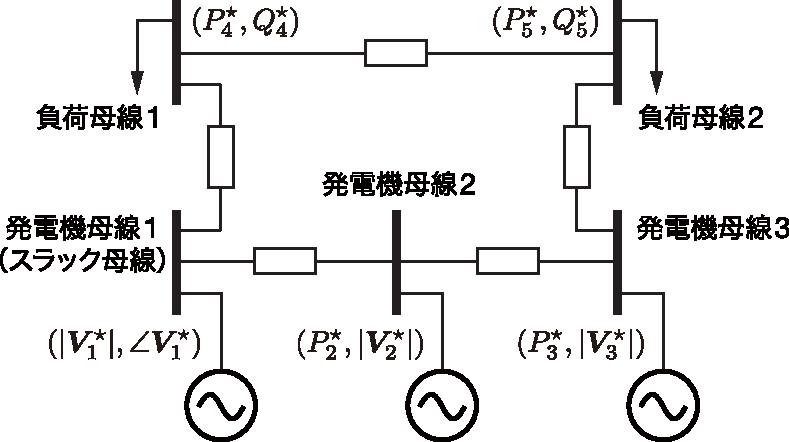
\includegraphics[width = .7\linewidth]{figs/powerflow}
%\medskip
%\caption{\textbf{3発電機母線と2負荷母線の潮流計算}}
%\label{fig:powerflow}
%\medskip
%\end{figure}


\begin{table}[h]
\medskip
\caption{\textbf{Data sheet and power flow calculation results (1)}} \label{table:pflow1}
 \centering
  {
  \begin{minipage}{0.49\linewidth}
    \centering
  \begin{tabular}{|c|c|c|c|c|c|c|}
   \hline
 & Bus 1 & Bus 2 & Bus 3 \\
   \hline 
   $P_i^{\star}$ & 0.5 & $-3$ & \\
   \hline
   $Q_i^{\star}$ &  & 0 & \\
   \hline
   $|\bm{V}_i^{\star}|$ & 2 & & 2 \\
   \hline
   $\angle \bm{V}_i^{\star}$ & & & 0 \\
   \hline
  \end{tabular}
  \subcaption{Data sheet}
  \end{minipage}
  \begin{minipage}{0.49\linewidth}
    \centering
  \begin{tabular}{|c|c|c|c|c|c|c|}
   \hline
 & Bus 1 & Bus 2 & Bus 3 \\
   \hline 
   $P_i^{\star}$ & & & 2.5006 \\
   \hline
   $Q_i^{\star}$ & 0.0157 & & 0.1388 \\
   \hline
   $|\bm{V}_i^{\star}|$ & & 1.9969 & \\
   \hline
   $\angle \bm{V}_i^{\star}$ & $-0.0490$ & $-0.0596$ & \\
   \hline
  \end{tabular}
   \subcaption{Power flow calculation results}
  \end{minipage}
  }
\end{table}


\begin{table}[h]
\medskip
\caption{\textbf{Data sheet and power flow calculation results (2)}} \label{table:pflow2}
 \centering
  {
  \begin{minipage}{0.49\linewidth}
    \centering
  \begin{tabular}{|c|c|c|c|c|c|c|}
    \hline
  & Bus 1 & Bus 2 & Bus 3 \\
    \hline 
    $P_i^{\star}$ &  & $-3$ & 0.5 \\
    \hline    
    $Q_i^{\star}$ &  & 0 & \\
    \hline
    $|\bm{V}_i^{\star}|$ & 2 & & 2 \\
    \hline
    $\angle \bm{V}_i$ & 0 & &  \\
    \hline
  \end{tabular}
   \subcaption{Data sheet}
  \end{minipage}
  \begin{minipage}{0.49\linewidth}
    \centering
  \begin{tabular}{|c|c|c|c|c|c|c|}
    \hline
    & Bus 1 & Bus 2 & Bus 3 \\
    \hline 
    $P_i^{\star}$ & 2.5158 & &  \\
    \hline
    $Q_i^{\star}$ & $-0.0347$ & & 0.1759 \\
    \hline
    $|\bm{V}_i^{\star}|$ & & 1.9918 & \\
    \hline
    $\angle \bm{V}_i^{\star}$ & & $-0.0538$ & $-0.0419$ \\
    \hline
  \end{tabular}
  \subcaption{Power flow calculation results}
  \end{minipage}
  }
\end{table}

\begin{example}{\textbf{Power flow calculation based on the datasheet}}\label{ex:pf3bus}
Let us consider the electrical power system model consisting of 3 bus bars
discussed in Example \ref{ex:derY}. For the admittance matrix of the power grid
of Equation \ref{eq:exY}, the admittance values of the two transmission lines
are set to be:
\begin{equation}\label{eq:rightlossless}
  \bm{y}_{12} = 1.3652 - \bm{j} 11.6041, \qquad
  \bm{y}_{23} =  - \bm{j} 10.5107
\end{equation}

Please note that the conductance (real part of $\bm{y}_{23}$) of the
transmission line that connects bus bar 2 and bus bar 3 is set to zero, so the
active power transmission loss on this line is zero.

First, let us consider a case where bus bar 1 is the generator bus, bus bar 2 is
the load bus, and bus bar 3 is the slack bus.  Specifically, we assume that the
values in Table \ref{table:pflow1}(a) are specified for each bus bar.  In this
case, the set of variable satisfying the simultaneous equations in Equation
\ref{eq:PQVgen} can be obtained as shown in Table \ref{table:pflow1}(b). The
transmission los in this case is:

\[
  P_1^{\star} + P_2^{\star} + P_3^{\star} = 6.2562\times 10^{-4},
  \qquad 
  Q_1^{\star} + Q_2^{\star} + Q_3^{\star} =1.5450  \times 10^{-1}
\]

The ratio of power transmission loss to the consumed power of the load is about
0.02\%, which is very small. The reason why the power transmission loss for the
active power is small is that most of the active power consumed by the load on
bus bar 2 (about 2.5 pu out of 3 pu) is supplied by the generator on bus bar 3,
and only 0.5 pu is supplied by the generator on bus bar 1. In other words, most
of the active power consumed by the load on bus bar 2 is supplied using the right
transmission line, which has no power transmission loss.

Next, consider the case where bus bar 1 is the slack bus, bus bar 2 is the load
bus, and bus bar 3 is the generator bus, and specify the variables for each bus
bar as shown in Table \ref{table:pflow2}(a). The result of the power flow
calculation in this case is shown in Table \ref{table:pflow2}(b). The power loss in
this case is given by:

\[
  P_1^{\star} + P_2^{\star} + P_3^{\star} = 1.5826 \times 10^{-2},
  \qquad 
  Q_1^{\star} + Q_2^{\star} + Q_3^{\star} =1.4120  \times 10^{-1}
\]

The ratio of power loss to consumed power of the load in this case is about
0.52\%. As compared to the previous example, it can be seen that the power loss
due to active power transmission has increased. This is because the majority of
the active power consumed by bus 2 is being supplied using the left transmission
line where power losses occur. On the other hand, it can also be seen that the
reactive power loss has decreased as compared to the previous example.
\end{example}

From Example \ref{ex:pf3bus}, it can be seen that the magnitude of the overall
transmission losses of the system varies depending on the power flow
distribution that is obtained. Generally, when supplying power using
transmission lines with a large conductance (or resistance) component, the
transmission losses of active power increase. As the transmission losses
increase, the generation cost, among other economic costs, also increases
because a larger amount of generation is required to supply the same amount of
consumed active power.

On the other hand, it is important to note that an economically efficient
steady-state power flow distribution may not necessarily correspond to a high
stability equilibrium point. Therefore, in practical applications, it is
important to search for better equilibrium points by considering trade-offs
between economic efficiency and stability. The process of searching for such
better equilibrium points is called \textbf{optimal power flow calculation} in
power system engineering. In this book, we discuss the relationship between the
selection of equilibrium points and stability in Chapters \ref{sec:staana} and
\ref{ch:stabcont}.

\subsection{The relationship between the admittance matrix and transmission
loss\advanced}

The following derivation provides a mathematical expression for transmission
losses in any power flow distribution for a general power network consisting of
$N$ buses. Assuming that the real and imaginary parts of the admittance matrix
$\bm{Y}$, which are the conductance matrix $G$ and susceptance matrix $B$,
respectively, are symmetric, appropriate constants $\phi_{ij}=\phi_{ji}$ and
$\psi_{ij}=\psi_{ji}$ can be used to represent $G_{ij}$ and $B_{ij}$,
respectively, as follows:

\begin{equation}\label{eq:GBrep}
  G_{ij} =
  \left\{
    \begin{array}{cl}
      \textstyle \sum_{j=1}^{N} \phi_{ij}, & i=j \\
      -\phi_{ij}, & i\neq j 
    \end{array}
  \right.
  \quad
  B_{ij}  =
  \left\{
    \begin{array}{cl}
      \textstyle - \sum_{j=1}^{N} \psi_{ij}, & i=j \\
      \psi_{ij}, & i\neq j 
    \end{array}
  \right.
\end{equation}

Here, $G_{ij}$ and $B_{ij}$ denote the $(i,j)$th element of the conductance
matrix $G$ and the susceptance matrix $B$, respectively. Equation \ref{eq:GBrep}
is equivalent to defining:

\[
  \phi_{ii}:= \sum_{j=1}^N G_{ij},\qquad
  \phi_{ij}:=-G_{ij},\qquad 
  \psi_{ii}:= - \sum_{j=1}^N B_{ij},\qquad 
  \psi_{ij}:=B_{ij}
\]

Using this expression, the following fact can be shown.

\begin{theorem}[Expression of transmission loss through bus bar voltage phasor]
\label{thm:PQ}
For equation \ref{eq:PQVgen}, the transmission losses of active and reactive
power for the entire system are defined as:

\begin{equation}
  L_{P}(t) := P_1(t) +\cdots P_N(t)
  ,\qquad
  L_Q(t) := Q_1(t) +\cdots Q_N(t)
\end{equation}

These transmission losses are given by:

\begin{equation}\label{eq:LPLQ}
  \spliteq{
    L_P(t) &= \sum_{i=1}^N \phi_{ii} |\bm{V}_{i}(t)|^2  +
    \sum_{i=1}^N \sum_{j=i+1}^N
    \phi_{ij} 
    W\bigl(\bm{V}_i(t),\bm{V}_j(t)\bigr)
    \\
    L_Q(t) &= \sum_{i=1}^N \psi_{ii} |\bm{V}_{i}(t)|^2  +
    \sum_{i=1}^N \sum_{j=i+1}^N
    \psi_{ij} 
    W\bigl(\bm{V}_i(t),\bm{V}_j(t)\bigr)
  }
\end{equation}

where the following is used:

\[
  W(\bm{V}_i,\bm{V}_j):=
  \left( |\bm{V}_i| - |\bm{V}_j| \right)^2 
  + 2 |\bm{V}_i| |\bm{V}_j| \bigl\{ 1-\sfcos (\angle \bm{V}_i- \angle \bm{V}_j) \bigr\}
\]
\end{theorem}

\begin{proof}
For simplification, time $t$ is omitted. Also, we denote $\angle\bm{V}_i- \angle
\bm{V}_j$ as $\angle \bm{V}_{ij}$. From Equation \ref{eq:PQVgen}, we have 
$\bm{Y}_{ij}= G_{ij} + \bm{j} B_{ij}$, and $\bm{Y}_{ij}=\bm{Y}_{ji}$, therefore:

\begin{equation*}
  \spliteq{
    \sum_{i=1}^N (P_i + \bm{j} Q_i)
    & =
    \sum_{i=1}^N \overline{\bm{Y}}_{ii} |\bm{V}_i|^2
    +
    \sum_{i=1}^N \sum_{j=i+1}^N
    \overline{\bm{Y}}_{ij}
    |\bm{V}_i| |\bm{V}_j| 
    \left(e^{ \bm{j} \angle \bm{V}_{ij} } + e^{ \bm{j} \angle \bm{V}_{ji} } \right) \\
    & =
    \sum_{i=1}^N \overline{\bm{Y}}_{ii} |\bm{V}_i|^2
    +
    2
    \sum_{i=1}^N \sum_{j=i+1}^N
    \overline{\bm{Y}}_{ij}
    |\bm{V}_i| |\bm{V}_j| 
    \sfcos \angle \bm{V}_{ij}
  }
\end{equation*}

Thus, using the notation of $G_{ij}$ and $B_{ij}$ from Equation \ref{eq:GBrep},
we obtain:

\begin{equation*}
  \spliteq{
    L_P &= 
    \sum_{i=1}^N \left(
    \sum_{j=1}^N \phi_{ij}
    \right)
    |\bm{V}_i|^2
    -
    2
    \sum_{i=1}^N \sum_{j=i+1}^N
    \phi_{ij}
    |\bm{V}_i| |\bm{V}_j| 
    \sfcos \angle \bm{V}_{ij} \\
    L_Q &= 
    \sum_{i=1}^N \left(
    \sum_{j=1}^N \psi_{ij}
    \right)
    |\bm{V}_i|^2
    -
    2
    \sum_{i=1}^N \sum_{j=i+1}^N
    \psi_{ij}
    |\bm{V}_i| |\bm{V}_j| 
    \sfcos \angle \bm{V}_{ij}
  }
\end{equation*}

where we focus on the first term of $L_P$. Because $\phi_{ij}=\phi_{ji}$, we
have:

\[
  \sum_{i=1}^N 
  \sum_{j=1}^N \phi_{ij}
  |\bm{V}_i|^2 = 
  \sum_{i=1}^N 
  \phi_{ii}|\bm{V}_i|^2
  +
  \sum_{i=1}^N 
  \sum_{j=i+1}^N \phi_{ij}
  |\bm{V}_i|^2
  +
  \sum_{i=1}^N 
  \sum_{j=i+1}^N \phi_{ij}
  |\bm{V}_j|^2
\]

If we rewrite the first term of $L_P$ using this, we can obtain:

\begin{equation*}
  \spliteq{
    L_P &= 
    \sum_{i=1}^N 
    \phi_{ii}|\bm{V}_i|^2
    +
    \sum_{i=1}^N 
    \sum_{j=i+1}^N \phi_{ij}
    \left(
      |\bm{V}_i|^2
      +
      |\bm{V}_j|^2
      -
      2 |\bm{V}_i| |\bm{V}_j| 
      \sfcos \angle \bm{V}_{ij}
    \right)
    \\
    &= 
    \sum_{i=1}^N 
    \phi_{ii}|\bm{V}_i|^2
    +
    \sum_{i=1}^N 
    \sum_{j=i+1}^N \phi_{ij}
    \left\{
      \left(
        |\bm{V}_i|
        -
        |\bm{V}_j|
      \right)^2
      +
      2 |\bm{V}_i| |\bm{V}_j| 
      (1-
      \sfcos \angle \bm{V}_{ij}
      )
    \right\}
  }
\end{equation*}

Therefore, $L_P$ can be expressed in the form of Equation \ref{eq:LPLQ}.
With the same steps, $L_Q$ can be expressed with the format of Equation
\ref{eq:LPLQ}.

\end{proof}

Theorem \ref{thm:PQ} shows that the discussion of electrical power loss in the
electrical power system of two bus bars shown in the Example \ref{ex:2buspf} can
be generalized to power systems consisting of any number of buses. Here, if we
express the admittance matrix $\bm{Y}$ as in Section \ref{sec:admathp}:

\[
  \bm{Y}=\bm{Y}_0 + \bm{j} \sfdiag(\Cgi)_{i\in \{1,\ldots,N\} }
\]

In this case, it is known that $\bm{Y}_0 \mathds{1}=0$, which means that the sum
of each row of the real and imaginary parts of $\bm{Y}_0$ is 0. Thus, for all
$i\in{1,\ldots,N}$:

\[
  \phi_{ii}=0,\qquad
  \psi_{ii}= - \Cgi
\]

Furthermore, since the conductance of each transmission line is nonnegative and
the susceptance is negative, it follows that $\phi_{ij}$ and $\psi_{ij}$ are
nonnegative for all $i\neq j$. Therefore, as long as $\phi_{ij}$ is not 0, loss
will always occur when transmitting active power between a bus bar $i$ and a bus
bar $j$.  This implies that the transmission loss of active power $L_P(t)$ is
positive at any time $t$ for the entire power system. Similarly, if $\Cgi$ is
sufficiently small; in other words, if the capacitance to ground of a
transmission line is sufficiently small, loss of reactive power $L_Q(t)$ is also
positive. In other words, connecting devices with capacitive characteristics to
the buses reduces the loss of reactive power.

\section{The steady state of generators achieving desired power
supply}\label{sec:paradef}

In this Section, we explain how to retroactively calculate the steady-state
values of the internal states and external inputs of generators, as well as the
parameter values of loads, to achieve the power flow state described by the
results of the power flow calculation explained in Step B of Section
\ref{sec:numstep}.

\subsection{The steady state of generators that achieves a desired supply of electric power}\label{sec:stagen}

Let us consider a generator model that inputs the voltage phasor in Section
\ref{sec:genfund}. For simplicity of notation, subscripts $i$ have been
omitted:
\begin{equation}\label{eq:gendif_}
  \simode{
    \dot{\delta}&= \omega_0  \Delta \omega\\
    M   \Delta \dot{\omega}&= 
    - D \Delta\omega  
    - P
    +P_{{\rm mech}}
    \\
    \taud \dot{E} & = 
    -\tfrac{ \Xs }{ \Xt }E
    +\left(
    \tfrac{ \Xs }{ \Xt } -1
    \right)
    |\bm{V}| \sfcos (\delta - \angle \bm{V} ) 
    + V_{{\rm field}}
  }
\end{equation}

Here, if the active power and reactive power are the outputs:

\begin{equation}\label{eq:PQout_}
  P =  \frac{|\bm{V} | E}{ \Xt } \sfsin(\delta -  \angle \bm{V}), \qquad
  Q =  \frac{|\bm{V}|E}{ \Xt } \sfcos (\delta - \angle \bm{V})
  -\frac{|\bm{V}|^2}{ \Xt }
\end{equation}

The purpose here is to determine the steady-state values of the internal state
and external input values of a generator that are consistent with the given
constant values of active power, reactive power, and voltage phasor of the bus
to which the generator is connected, as the result of power flow calculation.
Specifically, let $(P^{\star},Q^{\star},|V^{\star}|,\angle \bm{V}^{\star})$
denote the given set of active power, reactive power, and absolute value and
phase of the voltage phasor. Then, the objective is to determine the
steady-state values of the internal state of the generator
$(\delta^{\star},E^{\star})$ and the external input values $(P_{{\rm
mech}}^{\star},V_{{\rm field}}^{\star})$ that satisfy the following set of
equations:

\begin{equation}\label{eq:P0Q0eq}
  \simode{
    p^{\star} &=  \tfrac{|v^{\star}| e^{\star}}{ \Xt } \sfsin(\delta^{\star} -  \angle \bm{v}^{\star}), \\
    q^{\star} & = \tfrac{|v^{\star}| e^{\star}}{ \Xt } \sfcos (\delta^{\star} -  \angle \bm{v}^{\star})
    -\tfrac{|v^{\star}|^2}{ \Xt }, \\
    0 & =  - p^{\star} +p_{{\rm mech}}^{\star}, \\
    0 & = 
    -\tfrac{ \Xs }{ \Xt }e^{\star}
    +\left(
    \tfrac{ \Xs }{ \Xt }-1
    \right)
    |v^{\star}| \sfcos (\delta^{\star} - \angle \bm{v}^{\star})
    + v_{{\rm field}}^{\star}
  }
\end{equation}

The set of equations in \ref{eq:P0Q0eq} represents the equilibrium point of the
generator model when the steady-state value of the angular frequency deviation
$\Delta \omega$ in equation \ref{eq:gendif_} is zero. Also, the given
$(P^{\star},Q^{\star},|V^{\star}|,\angle \bm{V}^{\star})$ corresponds to the
input and output values of the generator model for each bus.

The specific values of the steady-state internal states of the generator that
satisfy equation \ref{eq:P0Q0eq} are given by:
\begin{subequations}\label{eq:intssgen}
\begin{equation}
  \spliteq{
    \delta ^{\star} &= \angle \bm{v}^{\star}
    + \sfarctan \left( \frac{p^{\star}}{q^{\star} + \tfrac{ |\bm{v}^{\star}|^2}{ \Xt } } \right), 
    \\
    e^{\star} &= 
    \frac{ \Xt }{ |\bm{v}^{\star}| } \sqrt{ \left( q^{\star} + \frac{|\bm{v}^{\star}|^2}{ \Xt } \right)^2 + (p^{\star})^2 } 
  }
\end{equation}

The steady-state values of the mechanical and field inputs are:

\begin{equation}\label{eq:pmvfdss}
  \spliteq{
    p_{{\rm mech}}^{\star} &=    p^{\star}, \\
    v_{{\rm field}}^{\star} &=  \frac{ \tfrac{ \Xs }{ |\bm{v}^{\star}| } \left\{ \left( q^{\star} + \tfrac{|\bm{v}^{\star}|^2}{ \Xt } \right) 
    \left(q^{\star} + \tfrac{|\bm{v}^{\star}|^2}{ \Xs } \right) +(p^{\star})^2  \right\} }
    {  \sqrt{ \left( q^{\star} + \tfrac{|\bm{v}^{\star}|^2}{ \Xt } \right)^2 + (p^{\star})^2 }  }
  }
\end{equation}
\end{subequations}

Please refer to Section \ref{sec:gensspq} for the derivation process of these equations.

\subsection{Load Parameters for Achieving Desired Power Consumption}\label{sec:loadpara}

In this section, we explain how to set the parameters of the load model
described in Section \ref{sec:loadpr} to achieve the desired power consumption.
By eliminating the current phase using Equation \ref{eq:defPQVIi2}, the fixed
impedance model can be expressed as follows:

\begin{equation}\label{eq:lmodimp}
  p + \bm{j} q = -\frac{|\bm{v}|^2}{\overline{\bm{z}}_{\rm load}^{\star}} 
\end{equation}

Here, the subscript $i$ of the bus is omitted for simplicity. This can be
interpreted as the fixed impedance model of the load, where the current phase
$\bm{V}$ is the input and the active power $P$ and reactive power $Q$ are the
outputs. If the values of the active power and reactive power determined by
power flow calculations are represented as $P^{\star}$ and $Q^{\star}$,
respectively, and the absolute value of the voltage phase is represented as
$|\bm{V}^{\star}|$, then the real part (resistance) and imaginary part
(reactance) of the load impedance $\bm{z}_{\rm load}^{\star}$ can be calculated
as:

\begin{equation}\label{eq:lmodimppara}
  \operatorname{Re} [\bm{z}_{\rm load}^{\star}] = - \frac{ p^{\star} |\bm{v}^{\star}|^2 }{(p^{\star})^2 + (q^{\star})^2}
  ,\qquad
  \operatorname{Im} [\bm{z}_{\rm load}^{\star}] = - \frac{ q^{\star} |\bm{v}^{\star}|^2 }{(p^{\star})^2 + (q^{\star})^2}
\end{equation}

Similarly, for the fixed current model, since the equation can be expressed as:

\begin{equation}
  p + \bm{j} q = \overline{\bm{i}}_{\rm load}^{\star} |\bm{v}|
\end{equation}

The real and imaginary parts of the load current parameter can be calculated as:

\begin{equation*}
  \operatorname{Re} [\bm{i}_{\rm load}^{\star}] =\frac{p^{\star} }{|\bm{v}^{\star}|},\qquad
  \operatorname{Im} [\bm{i}_{\rm load}^{\star}] = -\frac{ q^{\star} }{|\bm{v}^{\star}|}
\end{equation*}

For the fixed power model, since the equation can be expressed as:

\begin{equation}
  p + \bm{j} q =
  p_{{\rm load}}^{\star} + \bm{j} q_{{\rm load}}^{\star} 
\end{equation}
%\end{subequations}

Then, clearly, the parameters are:

\begin{equation*}
  p_{\rm load}^{\star}=p^{\star}
  ,\qquad
  q_{\rm load}^{\star}=q^{\star}
\end{equation*}

By setting these parameter values in the load model, the steady-state flow state
obtained by power flow calculation can be achieved.

\subsection{mathematical relationship between generator internal state and
input/output\advanced}\label{sec:gensspq}

In the following, we mathematically analyze the internal state of the generator,
the active and reactive power provided to the bus bar, and voltage phasor of the
bus bar. We use the generator model discussed in Section \ref{sec:genmodadv}.
However, for ease of notation, we omit the subscript $i$ and use the model as
follows:

\begin{equation}\label{eq:gendif}
  \simode{
    \dot{\delta}&= \omega_0  \Delta \omega\\
    M   \Delta \dot{\omega}&= 
    - D \Delta\omega  
    - P
    +P_{{\rm mech}}
    \\
    \taud \dot{E} & = 
    -\tfrac{X_{{\rm d}}}{X_{{\rm d}}'}E
    +\left(
    \tfrac{X_{{\rm d}}}{X_{{\rm d}}'}-1
    \right)
    |\bm{V}| \sfcos (\delta - \angle \bm{V} ) 
    + V_{{\rm field}}
  }
\end{equation}

When the output is given as active and reactive power, we have:

\begin{equation}\label{eq:PQout}
  \spliteq{
    P &=  \frac{|\bm{V} | E}{X_{{\rm d}}'} \sfsin(\delta -  \angle \bm{V})
    -  
    \left( \frac{1}{X_{{\rm d}}'}  -  \frac{1}{X_{{\rm q}}} \right)
    |\bm{V}|^2 \sfsin( \delta - \angle \bm{V})\sfcos( \delta - \angle \bm{V}), \\
    Q &=  \frac{|\bm{V}|E}{X_{{\rm d}}'} \sfcos (\delta - \angle \bm{V})
    -|\bm{V}|^2 \left( \frac{\sfcos^2 (\delta - \angle \bm{V}) }{X_{{\rm d}}'} 
    + \frac{\sfsin^2 (\delta - \angle \bm{V})}{X_{{\rm q}}} \right)
  }
\end{equation}

Note that $X_{{\rm d}}'$ and $X_{{\rm q}}$ are equal to $\Xt$, and if we replace
$X_{\rm d}$ with $\Xs$, this model matches the generator model discussed in
Section \ref{sec:stagen}. When the output is given as current phasors, we have:

\begin{align}\label{eq:phVIsincosC2}
\spliteq{
 |\bm{I}| \sfcos (\delta -\angle \bm{I}) & =
\frac{|\bm{V}|}{X_{{\rm q}}}  \sfsin (\delta -\angle \bm{V}) , \\
|\bm{I}| \sfsin (\delta -\angle \bm{I})
& = \frac{E - |\bm{V}| \sfcos (\delta -\angle \bm{V}) }{X_{{\rm d}}'} 
}
\end{align}

Note that equations \ref{eq:PQout} and \ref{eq:phVIsincosC2} are equivalent
outputs, meaning that for any given $(\delta, E, |\bm{V}|, \angle \bm{V})$,
there exists a one-to-one relationship between $(P,Q)$ and $(|\bm{I}|, \angle
\bm{I})$.

The following facts are shown for this generator model.

\begin{lemma}[Relationship between generator internal states and
input/output]\label{lem:delVE}

Consider equation \ref{eq:PQout} as a system of equations in $\delta - \angle
\bm{V}$ and $E$. The solution is given by:
\begin{subequations}\label{eq:tandelV}
  \begin{align}
    \delta - \angle \bm{V} & = \sfarctan  \left( \frac{P}{Q + \tfrac{ |\bm{V}|^2}{X_{\rm q}} } \right) , \label{eq:tandelVa} \\
    E &= \frac{ \tfrac{X_{\rm d}'}{|\bm{V}| } \left\{ \left( Q + \tfrac{|\bm{V}|^2}{X_{\rm q}} \right) \left(Q + \tfrac{|\bm{V}|^2}{X_{\rm d}'} \right) +P^2  \right\} }{  \sqrt{ \left( Q + \tfrac{|\bm{V}|^2}{X_{\rm q}} \right)^2 + P^2 }  } \label{eq:tandelVb}
  \end{align}
  \end{subequations}
%\begin{align}\label{eq:tandelV}
%\spliteq{
%\delta(t) - \angle \bm{V}(t) & = \sfarctan  \left( \frac{P(t)}{Q(t) + \frac{ |\bm{V}(t)|^2}{X_{\rm q}} } \right) , \\
%E(t) &=
%\frac{ \frac{X_{\rm d}'}{|\bm{V}(t)| } \left\{ \left( Q(t) + \frac{|\bm{V}(t)|^2}{X_{\rm q}} \right) \left(Q(t) + \frac{|\bm{V}(t)|^2}{X_{\rm d}'} \right) +P^2(t)  \right\} }
%{  \sqrt{ \left( Q(t) + \frac{|\bm{V}(t)|^2}{X_{\rm q}} \right)^2 + P^2(t) }  }
%}
%\end{align}
where $|\bm{V}|\neq 0$.

Conversely, if we consider Equation \ref{eq:tandelV} as a system of equations in
$P$ and $Q$, the solution is given by Equation \ref{eq:PQout}.
\end{lemma}

\begin{proof}
First, we derive Equation \ref{eq:tandelV} from Equation \ref{eq:PQout}.
Multiplying $P$ by $\sfcos (\delta - \angle \bm{V})$ and $Q$ by $\sfsin (\delta
- \angle \bm{V})$ and taking the difference, we obtain:

\begin{equation*}
  P \sfcos (\delta - \angle \bm{V}) - Q \sfsin (\delta - \angle \bm{V})
  = \frac{|\bm{V}|^2}{X_{\rm q}} \sfsin (\delta - \angle \bm{V}) 
\end{equation*}

Dividing both sides by $\sfcos (\delta - \angle \bm{V})$, we obtain Equation
\ref{eq:tandelVa}.  Next, we show the relation of Euqtion \ref{eq:tandelVb}.
Rewriting $P$ and $Q$ in terms of $\bm{I}$ using the Equation
\ref{eq:defPQVIi2}, Equation \ref{eq:PQout} is equivalently transformed to
Equation \ref{eq:phVIsincosC2}. Furthermore, this is equivalent to:

\begin{equation}\label{eq:tmpVE}
  |\bm{V}|e^{\bm{j}(\delta - \angle \bm{V})}=E
  -X_{\rm d}' |\bm{I}| \sfsin (\delta - \angle \bm{I})
  + 
  \bm{j} X_{\rm q} 
  |\bm{I}| \sfcos (\delta - \angle \bm{I})
\end{equation}

The relationship in Equation \ref{eq:tandelVa} can be expressed in complex
numbers as:

\begin{equation*}
  \frac{ e^{\bm{j}(\delta - \angle \bm{V})} - e^{-\bm{j}(\delta - \angle \bm{V})}}
  {e^{\bm{j}(\delta - \angle \bm{V})} + e^{-\bm{j}(\delta - \angle \bm{V})}}
  = 
  \underbrace{
  \frac{P}{Q + \tfrac{ |\bm{V}|^2}{X_{\rm q}} }
  }_{\alpha}
  \bm{j}
\end{equation*}

Therefore, we obtain:
\begin{equation*}
  e^{-\bm{j}(\delta - \angle \bm{V})} = \frac{1-\alpha \bm{j}}{1+\alpha \bm{j}}
  e^{\bm{j}(\delta - \angle \bm{V})}
\end{equation*}

By considering the complex conjugate of Equation \ref{eq:defPQVIi2}, it can be
transformed into an equivalent form given by:

\begin{equation}\label{eq:IVPQ}
  |\bm{I}|e^{\bm{j}(\delta - \angle \bm{I})} = \frac{P+\bm{j}Q}{|\bm{V}|}  
  e^{\bm{j}(\delta - \angle \bm{V})}
\end{equation}

Then, by taking the complex conjugate of the above equation:

\begin{equation}\label{eq:IVPQc}
|\bm{I}|e^{-\bm{j}(\delta - \angle \bm{I})} = \frac{P-\bm{j}Q}{|\bm{V}|}  
\cdot \frac{1-\alpha \bm{j}}{1+\alpha \bm{j}}
e^{\bm{j}(\delta - \angle \bm{V})}
\end{equation}

From Equations \ref{eq:IVPQ} and \ref{eq:IVPQc}:
\begin{align*}
  |\bm{I}| \sfsin (\delta - \angle \bm{I})
  & =
  \frac{1}{|\bm{V}|} \cdot
  \frac{\alpha P +Q}{ 1+\alpha \bm{j} }e^{\bm{j}(\delta - \angle \bm{V})}, \\
  |\bm{I}| \sfcos (\delta - \angle \bm{I})
  & =
  \frac{1}{|\bm{V}|} \cdot
  \frac{ P - \alpha Q}{ 1+\alpha \bm{j} }e^{\bm{j}(\delta - \angle \bm{V})}
\end{align*}

By substituting these into Equation \ref{eq:tmpVE} and rewriting $\bm{I}$ in
terms of $P$ and $Q$, we can show that when Equation \ref{eq:tandelVa} holds,
Equation \ref{eq:PQout} is equivalent to:

\begin{equation}\label{eq:Etran}
  E=
  \frac{X_{\rm d}'}{|\bm{V}| } 
  \left\{
    \left(Q + \frac{|\bm{V}|^2}{X_{\rm q}} \right) \left(Q + \frac{|\bm{V}|^2}{X_{\rm d}'} \right) +P^2
  \right\}
  \frac{  Q + \tfrac{|\bm{V}|^2}{X_{\rm q}} - \bm{j} P }{   \left( Q + \tfrac{|\bm{V}|^2}{X_{\rm q}} \right)^2 + P^2   }
  e^{\bm{j}(\delta - \angle \bm{V})}
\end{equation}

Here, we have used the fact that from Equation \ref{eq:tandelVa}:

\begin{equation*}
  Q + \frac{|\bm{V}|^2}{X_{\rm q}} - \bm{j} P
  = 
  \left|Q + \frac{|\bm{V}|^2}{X_{\rm q}} - \bm{j} P \right|
  e^{-\bm{j}(\delta - \angle \bm{V})}
\end{equation*}

Furthermore, since $|E|=E$ and

\[
\left( Q + \frac{|\bm{V}|^2}{X_{\rm q}} \right)^2 + P^2
=
\left|Q + \frac{|\bm{V}|^2}{X_{\rm q}} - \bm{j} P \right|^2
\]
Equation \ref{eq:tandelVb} can be obtained.

We can follow the reverse steps to derive Equation \ref{eq:PQout} from Equation
\ref{eq:tandelV}. Using Equation \ref{eq:tandelVa}, we can replace the $E$ in
Equation \ref{eq:tandelVb} with the expression in Equation \ref{eq:Etran}. As
mentioned earlier, when Equation \ref{eq:tandelVa} holds, Equation
\ref{eq:Etran} is equivalent to Equation \ref{eq:PQout}.
\end{proof}

Lemma \ref{lem:delVE} shows that there is a one-to-one relationship between the
pairs $(\delta - \angle \bm{V},E)$ and $(P,Q)$. Specifically, it shows that the
internal state of generators $(\delta,E)$ can be uniquely determined from the
input/output $(|\bm{V}|,\angle \bm{V})$ or $(P,Q)$. Please note that the
relationship in Equation (\ref{eq:tandelV}) holds at any time $t$, regardless of
whether the system is in steady-state or transient. The following theorem gives
a relationship that holds between the input, output, and internal state under a
steady state of generators.

\begin{theorem}[Relationship between generator internal states and input/output
in steady state] \label{thm:stst}

Consider the generator model given by Equations \ref{eq:gendif} and
\ref{eq:PQout}. Let $\bm{V}^{\star}$, $\Delta \omega^{\star}$, $\angle
\bm{V}^{\star}$, $P^{\star}$, and $Q^{\star}$ be real constants. Let us assume
the inputs of mechanical torque and field voltage are constants given by:

\begin{subequations}\label{eq:allinputs}
\begin{align}\label{eq:PmVfd}
  \spliteq{
    P_{{\rm mech}}(t) &=   D \Delta \omega^{\star}  + P^{\star}, \\
    V_{{\rm field}}(t) &=  \frac{ \tfrac{X_{\rm d}}{ |\bm{V}^{\star}| } \left\{ \left( Q^{\star} + \tfrac{|\bm{V}^{\star}|^2}{X_{\rm q}} \right) 
    \left(Q^{\star} + \tfrac{|\bm{V}^{\star}|^2}{X_{\rm d}} \right) +(P^{\star})^2  \right\} }
    {  \sqrt{ \left( Q^{\star} + \tfrac{|\bm{V}^{\star}|^2}{X_{\rm q}} \right)^2 + (P^{\star})^2 }  }
  }
\end{align}
and the input due to the voltage phase angle of the bus are given by:

\begin{align}\label{eq:busvolin}
  |\bm{V}(t)|=|\bm{V}^{\star}|,\qquad
  \angle \bm{V}(t) = \omega_0 \Delta \omega^{\star} t + \angle \bm{V}^{\star}
\end{align}
\end{subequations}

where $\omega_0$ is the nominal frequency. Then, in steady state, the rotor
angle, angular frequency deviation, and internal voltage are given by

\begin{equation}\label{eq:inicon}
  \spliteq{
    \delta (t) &= \angle \bm{V}(t)
    + \sfarctan \left( \frac{P^{\star}}{Q^{\star} + \tfrac{ |\bm{V}^{\star}|^2}{X_{\rm q}} } \right), 
    \\
    \Delta \omega(t) &= \Delta \omega^{\star},
    \\
    E(t) &= \frac{ \tfrac{X_{\rm d}'}{ |\bm{V}^{\star}| } \left\{ \left( Q^{\star} + \tfrac{|\bm{V}^{\star}|^2}{X_{\rm q}} \right) 
    \left(Q^{\star} + \tfrac{|\bm{V}^{\star}|^2}{X_{\rm d}' } \right) +(P^{\star})^2  \right\} }
    {  \sqrt{ \left( Q^{\star} + \tfrac{|\bm{V}^{\star}|^2}{X_{\rm q}} \right)^2 + (P^{\star})^2 }  }
  }
\end{equation}

Furthermore, the active and reactive power supplied to bus bars are constants
and given by:

\begin{align}\label{eq:PtQt}
P(t)=P^{\star},\qquad
Q(t)=Q^{\star}
\end{align}
\end{theorem}

\begin{proof}
First, we demonstrate that Equation \ref{eq:PtQt} holds for the output under the
assumption that Equation \ref{eq:inicon} is a solution to the differential
equation in Equation \ref{eq:gendif} with the input given by Equation
\ref{eq:allinputs}. As shown in Lemma \ref{lem:delVE}, considering Equation
\ref{eq:inicon} as equations for $P^{\star}$ and $Q^{\star}$, their solutions
are given by

\begin{equation*}
  \spliteq{
    P^{\star} &=  \frac{|\bm{V}^{\star}| E(t)}{X_{{\rm d}}'} \sfsin\left(\delta(t) -  \angle \bm{V}(t)\right) 
    \\
    & -  
    \left( \frac{1}{X_{{\rm d}}'}  -  \frac{1}{X_{{\rm q}}} \right)
    |\bm{V}^{\star}|^2 \sfsin\left( \delta(t) - \angle \bm{V}(t) \right) \sfcos\left( \delta(t) - \angle \bm{V}(t) \right), 
    \\
    Q^{\star} &=  \frac{|\bm{V}^{\star}| E(t)}{X_{{\rm d}}'} \sfcos \left( \delta(t) - \angle \bm{V}(t) \right)
    \\
    & - |\bm{V}^{\star}|^2 \left( \frac{\sfcos^2 \left( \delta(t) - \angle \bm{V}(t) \right) }{X_{{\rm d}}'} 
    + \frac{\sfsin^2 \left( \delta(t) - \angle \bm{V}(t) \right)}{X_{{\rm q}}} \right)
  }
\end{equation*}
which implies Equation \ref{eq:PtQt}.

Next, we verify that Equation \ref{eq:inicon} is a solution to the differential
equation in Equation \ref{eq:gendif} with the input given by equation
\ref{eq:allinputs}. The differential equation for $\delta$ and $\Delta \omega$
in Equation \ref{eq:gendif} is equivalent to

\begin{equation*}
\frac{M}{\omega_0} \ddot{\delta}(t) + \frac{D}{\omega_0} \dot{\delta}(t)
+ P(t) - P_{{\rm mech}}(t) = 0
\end{equation*}

If we substitute the expressions for $P_{{\rm mech}}(t)$ from Equation
\ref{eq:PmVfd}, $P(t)$ from Equation \ref{eq:PtQt}, and $\delta(t)$ from
Equation \ref{eq:inicon} into the relationship given by Equation
\ref{eq:busvolin}, we can see that this differential equation is satisfied.
Similarly, by substituting the expressions for $V_{{\rm field}}(t)$ from
Equation \ref{eq:PmVfd}, $\delta(t) - \angle \bm{V}(t)$, and $E(t)$ from
Equation \ref{eq:inicon} into Equation \ref{eq:gendif}, we can see that the
differential equation for $E$ is satisfied.  Here, we use the fact that:

\begin{equation*}
  \sfcos \left( \sfarctan \left( \frac{P^{\star}}{Q^{\star} + \tfrac{ |\bm{V}^{\star}|^2}{X_{\rm q}} } \right) \right) =
  \frac{ Q^{\star} + \tfrac{|\bm{V}^{\star}|^2}{X_{\rm q}} }
  {  \sqrt{ \left( Q^{\star} + \tfrac{|\bm{V}^{\star}|^2}{X_{\rm q}} \right)^2 + (P^{\star})^2 }  }
\end{equation*}
From the above, we prove Theorem \ref{thm:stst}.

\end{proof}

From Theorem \ref{thm:stst}, we can determine the values of mechanical input
$P_{\rm mech}^{\star}$ and field input $V_{\rm field}^{\star}$ that are
necessary to achieve the voltage phase, active power, and reactive power of the
bus bars determined by power flow calculation, as well as the steady-state
behavior of internal states $(\delta, E)$ at that time. Note that in Equation
\ref{eq:busvolin}, the phase of the voltage phasor is not a constant, but the
steady-state value of the angular frequency deviation $\Delta \omega^{\star}$,
which usually should be set to zero as a constant with practical significance,
is determined only by the value of $\angle \bm{V}^{\star}$ obtained from the
power flow calculation. Clearly, when $\Delta \omega^{\star}=0$,

\begin{equation*}
  P_{{\rm mech}}(t) =    P^{\star},\qquad
  \delta (t)  = \angle \bm{V}^{\star}
  + \sfarctan \left( \frac{P^{\star}}{Q^{\star} + \tfrac{ |\bm{V}^{\star}|^2}{X_{\rm q}} } \right)
\end{equation*}

From the above discussion, we can see that even if we determine
$(P^{\star},Q^{\star},|\bm{V}^{\star}|,\angle \bm{V}^{\star})$ by power flow
calculation without considering the dynamic characteristics of the generator, we
can uniquely calculate $(P_{\rm mech}^{\star},V_{\rm field}^{\star})$ that are
consistent with them. This result leads to Equation (\ref{eq:intssgen}).

Furthermore, the following theorem gives an equivalence relation between the
inputs and internal states in steady-state of the generator.

\begin{theorem}[Equivalence relation between input/output and internal state of
generator] \label{thm:outst}

For the generator model given by Equations \ref{eq:gendif} and \ref{eq:PQout},
the necessary and sufficient conditions for Equations \ref{eq:domdE} to hold for
all $t \geq 0$ are that Equations \ref{eq:dPdQ} hold for all $t \geq 0$, where

\begin{equation}\label{eq:domdE}
  \frac{d^2 \delta}{dt^2}(t)=0
  ,\quad
  \frac{dE}{dt}(t)=0
  ,\quad
  \frac{d P_{\rm mech}}{dt}(t)=0
  ,\quad
  \frac{d V_{\rm field}}{dt}(t)=0
\end{equation}
%\begin{align}\label{eq:domdE}
%\frac{d^2 \delta}{dt^2}=0
%,\qquad
%\frac{dE}{dt}=0
%,\qquad
%\frac{d P_{\rm mech}}{dt}=0
%,\qquad
%\frac{d V_{\rm field}}{dt}=0
%\end{align}
%であるための必要十分条件は
and
\begin{equation}\label{eq:dPdQ}
  \frac{dP}{dt}(t)=0
  ,\quad
  \frac{dQ}{dt}(t)=0
  ,\quad
  \frac{d|\bm{V}|}{dt}(t)=0
  ,\quad
  \frac{d^2 \angle \bm{V}}{dt^2}(t)=0
\end{equation}

Moreover, when equations \ref{eq:domdE} or \ref{eq:dPdQ} hold, the following
holds for all $t \geq 0$:

\begin{equation}\label{eq:frer}
  \Delta \omega(t)= \frac{1}{\omega_0}\frac{d \angle \bm{V}}{dt}(t)
\end{equation}
which is a constant.

\end{theorem}

\begin{proof}
First, we show that if Equation \ref{eq:domdE} holds, then Equation
\ref{eq:dPdQ} also holds. From Equation \ref{eq:gendif}, since $\Delta \omega$,
$E$, $P_{\rm mech}$, and $V_{\rm field}$ are all constants, we can see that $P$
and $|\bm{V}|\sfcos (\delta - \angle \bm{V})$ are also constants. Therefore,
from the two equations in Equation \ref{eq:PQout}, we can see that $Q$ and
$|\bm{V}|\sfsin (\delta - \angle \bm{V})$ are also constants. Additionally,

\begin{equation*}
  |\bm{V}|^2\sfcos^2 (\delta - \angle \bm{V}) +
  |\bm{V}|^2\sfsin^2 (\delta - \angle \bm{V}) = |\bm{V}|^2
\end{equation*}
and since the left-hand side is constant, we can see that $|\bm{V}|$ is also
constant. Furthermore, in the first equation of Equation \ref{eq:tandelV}, the
right-hand side is constant, so the derivatives of $\angle \bm{V}$ and $\delta$
are equal for any order. Therefore, we have

\begin{equation*}
\frac{d^2 \angle \bm{V}}{dt^2} = \frac{d^2 \delta}{dt^2} =0
\end{equation*}

Next, we show that if Equation \ref{eq:dPdQ} holds, then Equation \ref{eq:domdE}
also holds. From Equation \ref{eq:tandelV}, we know that $E$ is constant and
that the second derivative of $\delta$ is 0, which means that $\Delta \omega$ is
constant. Therefore, from Equation \ref{eq:gendif}, since $P$ and
$|\bm{V}|\sfcos (\delta - \angle \bm{V})$ are constants, we can see that $P_{\rm
mech}$ and $V_{\rm field}$ are also constants. Equation \ref{eq:frer} is
obvious from the fact that the derivatives of $\angle \bm{V}$ and $\delta$ are
equal.
\end{proof}

As Theorem \ref{thm:outst} shows, the fact that the external inputs $(P_{\rm
mech},V_{\rm field})$ to the generator are constant and the internal states
$(\delta,E)$ are in a steady state is equivalent to the input/output
$(P,Q,|\bm{V}|,\angle \bm{V})$ to the bus being in a steady state. Therefore,
the procedures for power flow calculations that determine the active and
reactive power and voltage phase angles for each bus are mathematically
equivalent to searching for one of the equilibrium points of the power system
model, assuming that all internal states and external inputs of the generators
are in steady state. This is the steady-state of the entire power system.

\section{Time Response Calculation of Power System Model}\label{sec:numsimtr}

In this Section, we explain a method to calculate the time response of the
electric power system model explained as Step C in Section \ref{sec:numstep}.
We will also numerically analyze the behavior of the electrical power system
against several disturbances.

\subsection{Initial Value Response}

In this section, we explain the method for calculating the time response of the
power system model, which was described as Step C in Section \ref{sec:numstep}.
We also numerically analyze the behavior of the power system model in response
to several disturbances.

By following the procedures outlined in Sections \ref{sec:powflow} and
\ref{sec:paradef}, the equilibrium point of the power system model can be
obtained as a steady-state where all generator frequency deviations are zero.
Specifically, by using the bus variables determined in the power flow
calculation, the initial values of the internal states and external inputs of
each generator model, as shown in Theorem \ref{thm:stst}, can be set. In
addition, the constants derived in Section \ref{sec:loadpara} can be set for
each load model. By doing so, the differential-algebraic equation system
representing the power system model is in equilibrium at the given steady-state
power flow condition.

In particular, if the obtained equilibrium point is stable in a meaningful
sense, then even if some perturbation occurs in the internal states of the
generators, the internal states of the power system model will asymptotically
converge to the original steady-state values. We confirm this fact in the
following example.

\begin{table}[h]
\medskip
 \caption{\textbf{Steady-state values of generators for flow calculation results of Table \ref{table:pflow1}}}
 \label{table:genst13a}
 \centering
  \begin{tabular}{ccccccccc}
   \hline
$i$ &  $P_{{\rm mech}i}^{\star}$~[pu] & $V_{{\rm filed}i}^{\star}$~[pu] & $\delta_i^{\star}$~[rad] & $\Delta \omega_i^{\star}$~[pu] & $E_i^{\star}$~[pu] \\
   \hline \hline
1 & $0.5000$ & 2.0442 & 0.0670 & 0 & 2.0210 \\
3 & $2.5006$ & 2.5062 & 0.3870 & 0 & 2.2097 \\
   \hline
  \end{tabular}
\end{table}

\begin{table}[h]
\medskip
 \caption{\textbf{Steady-state values of generators for flow calculation results of Table \ref{table:pflow2}}}
 \label{table:genst13b}
 \centering
  \begin{tabular}{cccccccc}
   \hline
$i$ &  $P_{{\rm mech}i}^{\star}$~[pu] & $V_{{\rm filed}i}^{\star}$~[pu] & $\delta_i^{\star}$~[rad] & $\Delta \omega_i^{\star}$~[pu] & $E_i^{\star}$~[pu] \\
   \hline \hline
1 & $2.5158$ & 2.7038 & 0.5356 & 0 & 2.3069 \\
3 & $0.5000$ & 2.1250 & 0.0390 & 0 & 2.0654 \\
   \hline
  \end{tabular}
\end{table}


\begin{example}{\textbf{Initial response of the electrical power system
model}}\label{ex:inires}
Let us consider the electrical power system model consisting of three bus bars
handled in the Example \ref{ex:pf3bus}.  Let us consider a situation where the
generator model of Equation \ref{eq:gendif_} is connected to bus bar 1 and bus
bar 3, and a load model with constant impedance of Equation \ref{eq:lmodimp} is
connected to bus bar 2.  For the generator model, we use the constants for
generator 1 and generator 2 presented in \ref{table:genparams}.

For the two results of the power flow calculation in \ref{table:pflow1} and
\ref{table:pflow2}, we calculate the steady values of mechanical torque, field
voltage, rotor argument, and interval voltage for generator 1 and generator 2
based on Equation (\ref{eq:intssgen}).  The calculated steady values are shown
in \ref{table:genst13a} and \ref{table:genst13b}.  Similarly, if we back
calculate the load impedance based on Equation \ref{eq:lmodimppara}, it can be
obtained as in the first row of \ref{table:loadpara1} and \ref{table:loadpara2}.
Please note that, depending on the result of the power flow calculation, the
internal state of the generators, the steady value of the external input, and
the load impedance vary.

Let us perturb the steady value of the internal state of the generators as the
initial value.  Specifically:

\begin{align}\label{eq:exdelE0_}
\mat{
\delta_1(0) \\
\delta_3(0) 
}
 =
\mat{
\delta_1^{\star} + \tfrac{\pi}{6} \\
\delta_3^{\star} 
},\qquad
\mat{
E_1(0) \\
E_3 (0)
}
 =
\mat{
E^{\star}_1 +0.1 \\
E^{\star}_3 
}
\end{align}
The initial value of the frequency deviation is 0.  Figure \ref{fig:P13ini}
shows the initial value response of the frequency deviation corresponding to the
two power flow calculations at this time.  The solid blue line represents the
frequency deviation of generator 1, while the broken red line is the frequency
deviation of generator 3.  With either one of the steady power flow
distributions, oscillations with a similar frequency were generated.  Since the
system frequency was set to 60 [Hz], a frequency deviation of $0.015$ [pu] is
equal to 0.9 [Hz].
\end{example}

\begin{table}[h] \medskip
 \centering
  {
  \begin{minipage}{0.49\linewidth}
  \caption{\textbf{Impedance value of load~[pu]}} \label{table:loadpara1}
    \centering
  \begin{tabular}{crrrccc}
   \hline
   Load &  $\real [\bm{z}_{{\rm load}2}^{\star}]$ & $\imag [\bm{z}_{{\rm load}2}^{\star}]$ \\
   \hline \hline
   Steady-state & 1.3293 & 0 \\
   Increased laod & 1.3426 & 0 \\
   Decreased load & 1.3160 & 0 \\
   \hline
  \end{tabular}
  \subcaption{Results of power flow calculation for Table\ref{table:pflow1}}
  \end{minipage}
  \begin{minipage}{0.49\linewidth}
  \caption{\textbf{Impedance value of load~[pu]}} \label{table:loadpara2}
    \centering
  \begin{tabular}{crrrrccccc}
   \hline
   Load &  $\real [\bm{z}_{{\rm load}2}^{\star}]$ & $\imag [\bm{z}_{{\rm load}2}^{\star}]$ \\
   \hline \hline
   Steady-state & 1.3224 & 0\\
   Increased load & 1.3356 & 0 \\
   Decreased load & 1.3092 & 0 \\
   \hline
  \end{tabular}
   \subcaption{Results of power flow calculation for Table \ref{table:pflow2}}
  \end{minipage}
  }
\end{table}



\begin{figure}[t]
  \centering
  {
  \begin{minipage}{0.49\linewidth}
    \centering
    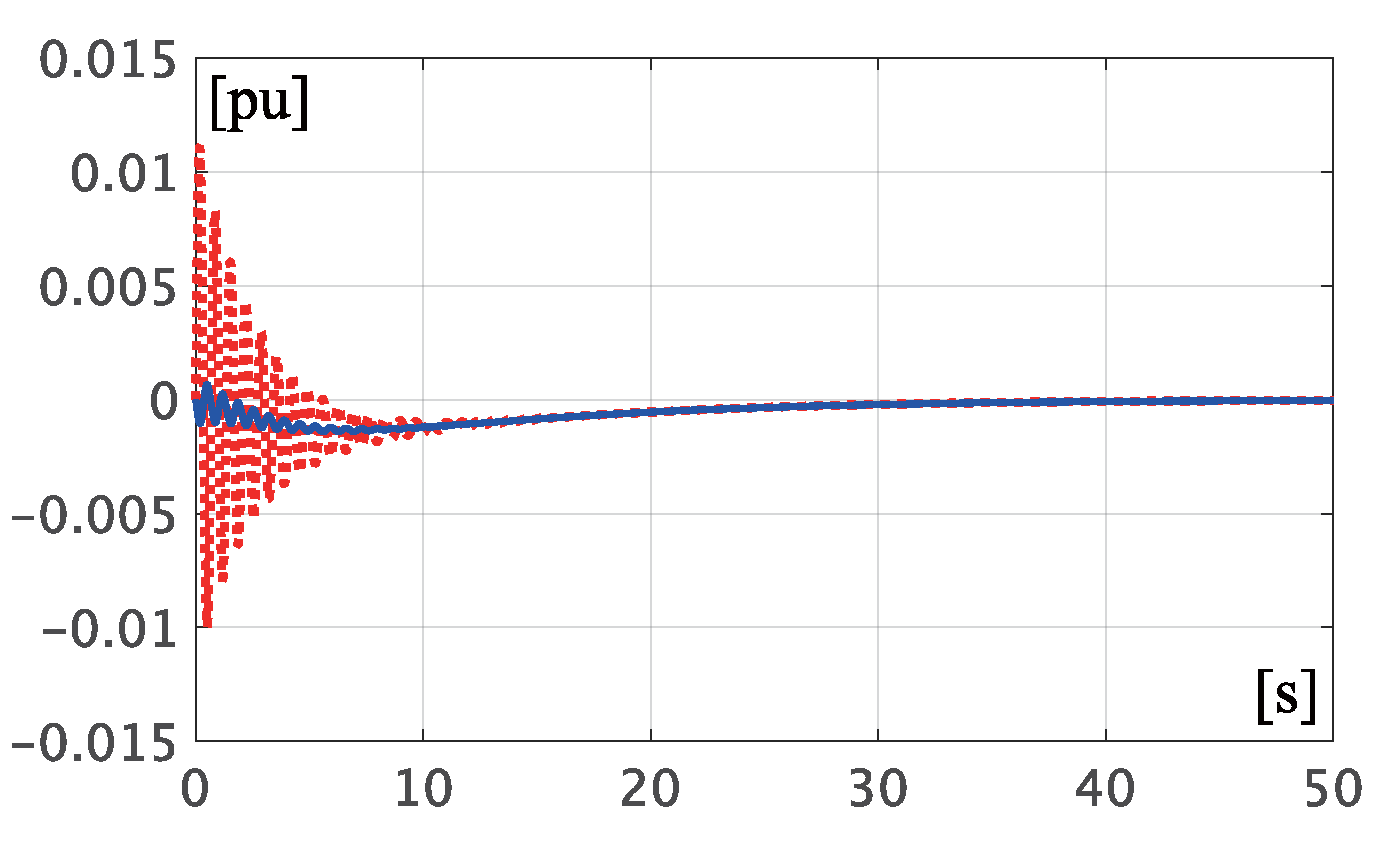
\includegraphics[width = 1.0\linewidth]{figs/P1ini}
    \subcaption{Steady-state power flow of Table \ref{table:pflow1}}
  \end{minipage}
  \begin{minipage}{0.49\linewidth}
    \centering
    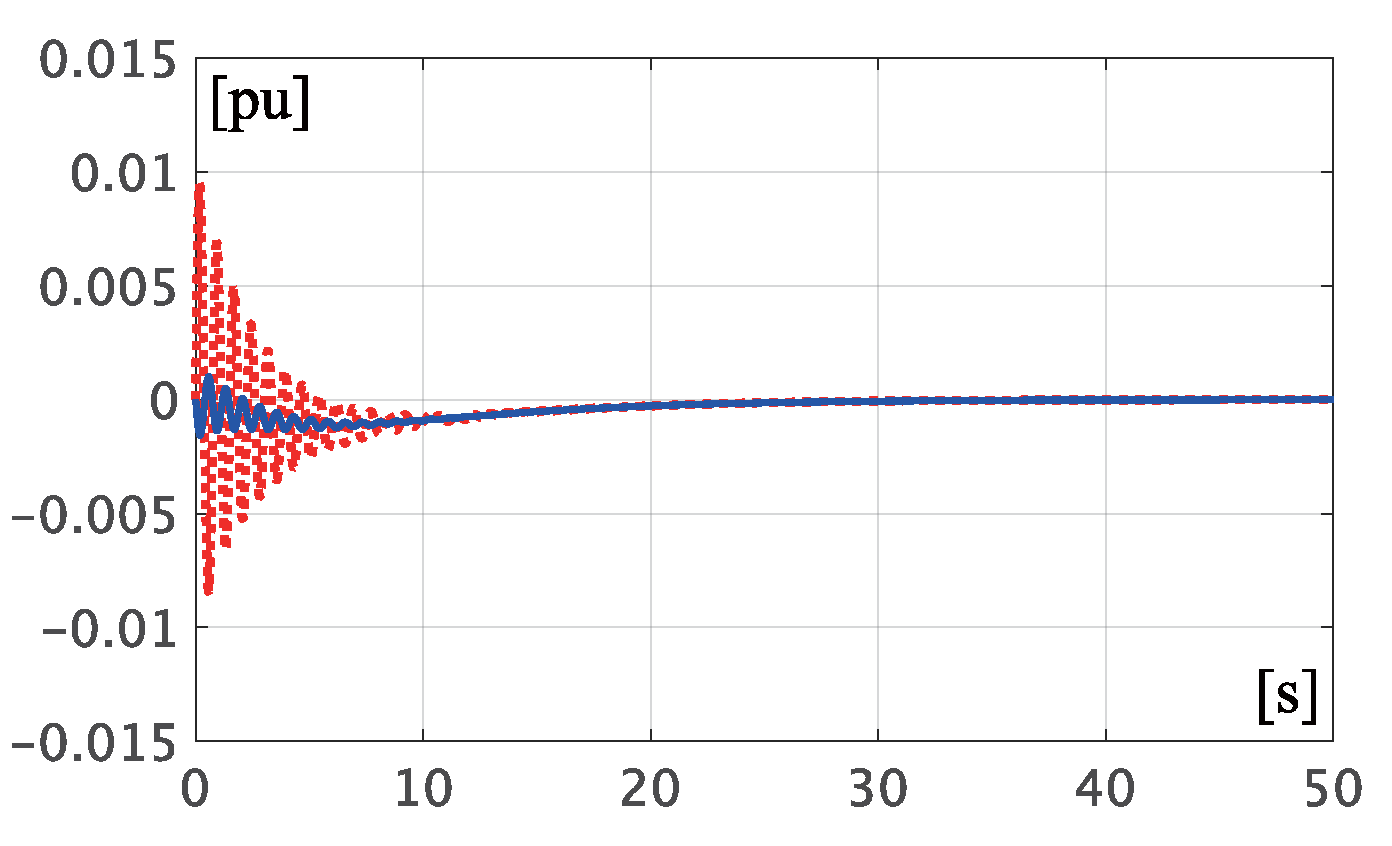
\includegraphics[width = 1.0\linewidth]{figs/P3ini}
    \subcaption{Steady-state power flow of Table \ref{table:pflow2}}
  \end{minipage}
  \medskip
  \caption{\textbf{Time response of frequency deviation for initial value
  disturbance}
  \\ \centering(Solid blue line: $\Delta \omega_1$, Dashed red line:$\Delta \omega_3$)}
  \label{fig:P13ini}
  }
\medskip
\end{figure}

\subsection{Response to Parameter Variations of the Load
Model}\label{sec:resldpara}

For a power system model in steady-state, if any of the constants in the load
model are changed, the values of the voltage and current phases at all buses
generally change. At this point, the power supply and demand in the entire
system generally no longer balance, so unless the value of the mechanical input
is appropriately modified according to the given excitation input value, the
angular frequency deviation of each generator will not converge to zero. Let's
verify this in the following example.

\begin{example}[Time Response of Power System Model to Load Impedance
Changes]\label{ex:loadpv}

Let us calculate the time response of the angular frequency deviation when the
load impedance value changes under the same setting as Example \ref{ex:inires}.
Specifically, we calculate the time response by increasing or decreasing
the resistance of the load by 1\% based on the results of the power flow
calculation. The increased and decreased load impedance values are shown in the
second and third rows of Tables \ref{table:loadpara1} and \ref{table:loadpara2},
respectively.

The calculation results are shown in Figures \ref{fig:P1load} and
\ref{fig:P3load}. The solid blue line represents the angular frequency
deviation of generator 1, and the dashed red line represents that of generator
3. In all cases, it can be seen that the angular frequency deviations of the two
generators change in sync. Also, since increasing the resistance generally
increases the consumption of active power, the frequency of the generators
decreases. The opposite is true when the resistance is decreased. It should be
noted that since the mechanical input of the generators is fixed at the value
before the change in resistance, the balance of active power supply and demand
is not maintained, and the steady-state value of the angular frequency deviation
is nonzero. Furthermore, although the ratio of the change in load resistance is
the same in both Figures \ref{fig:P1load} and \ref{fig:P3load}, the resulting
values of the angular frequency deviation are different. This suggests that the
sensitivity (stability) to disturbances changes depending on how the equilibrium
point of the power system model is chosen.

\end{example}

\begin{figure}[t]
  \centering
  {
  \begin{minipage}{0.49\linewidth}
    \centering
    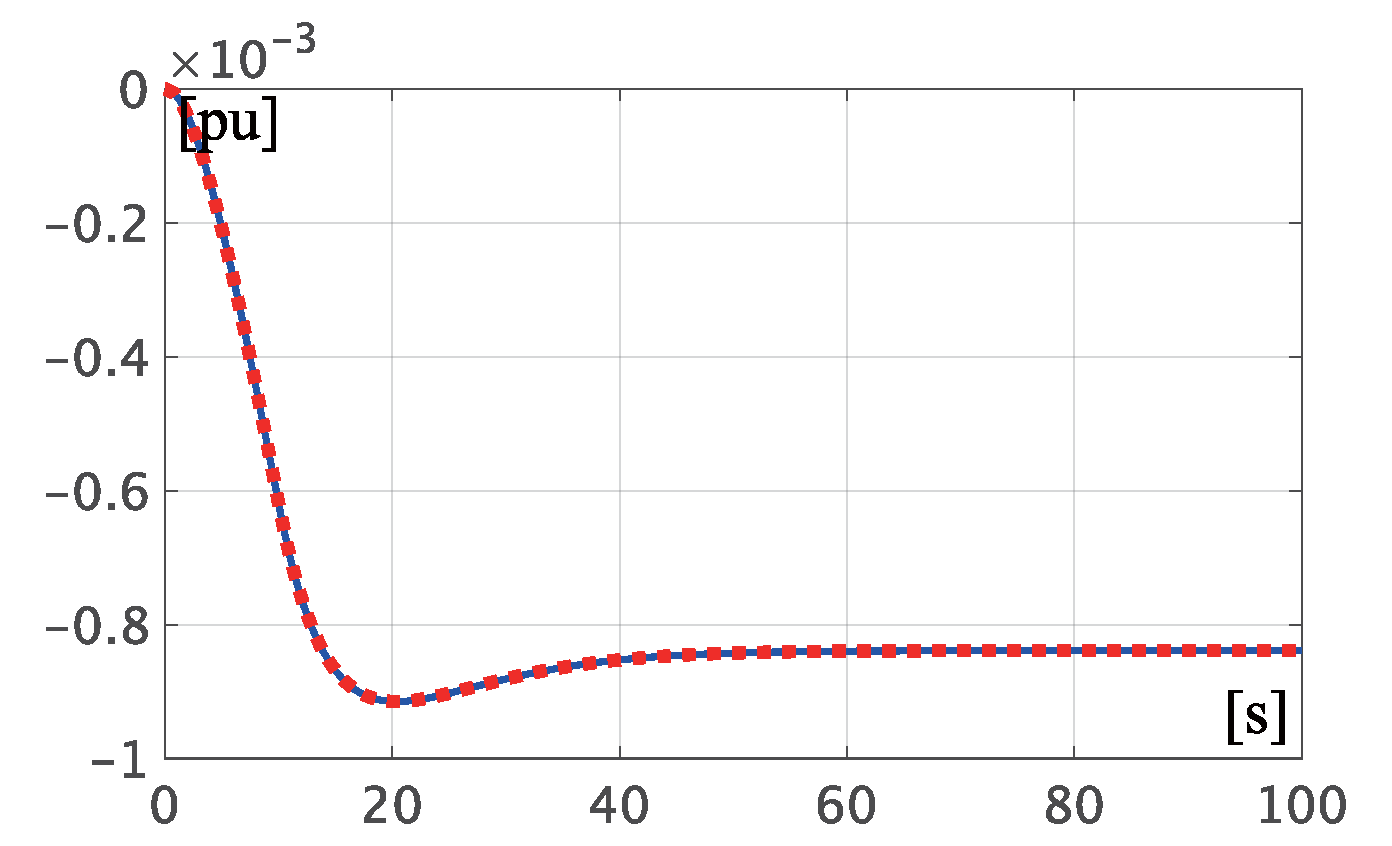
\includegraphics[width = 1.0\linewidth]{figs/P1mi}
    \subcaption{If resistance is increased by 1\%}
  \end{minipage}
  \begin{minipage}{0.49\linewidth}
    \centering
    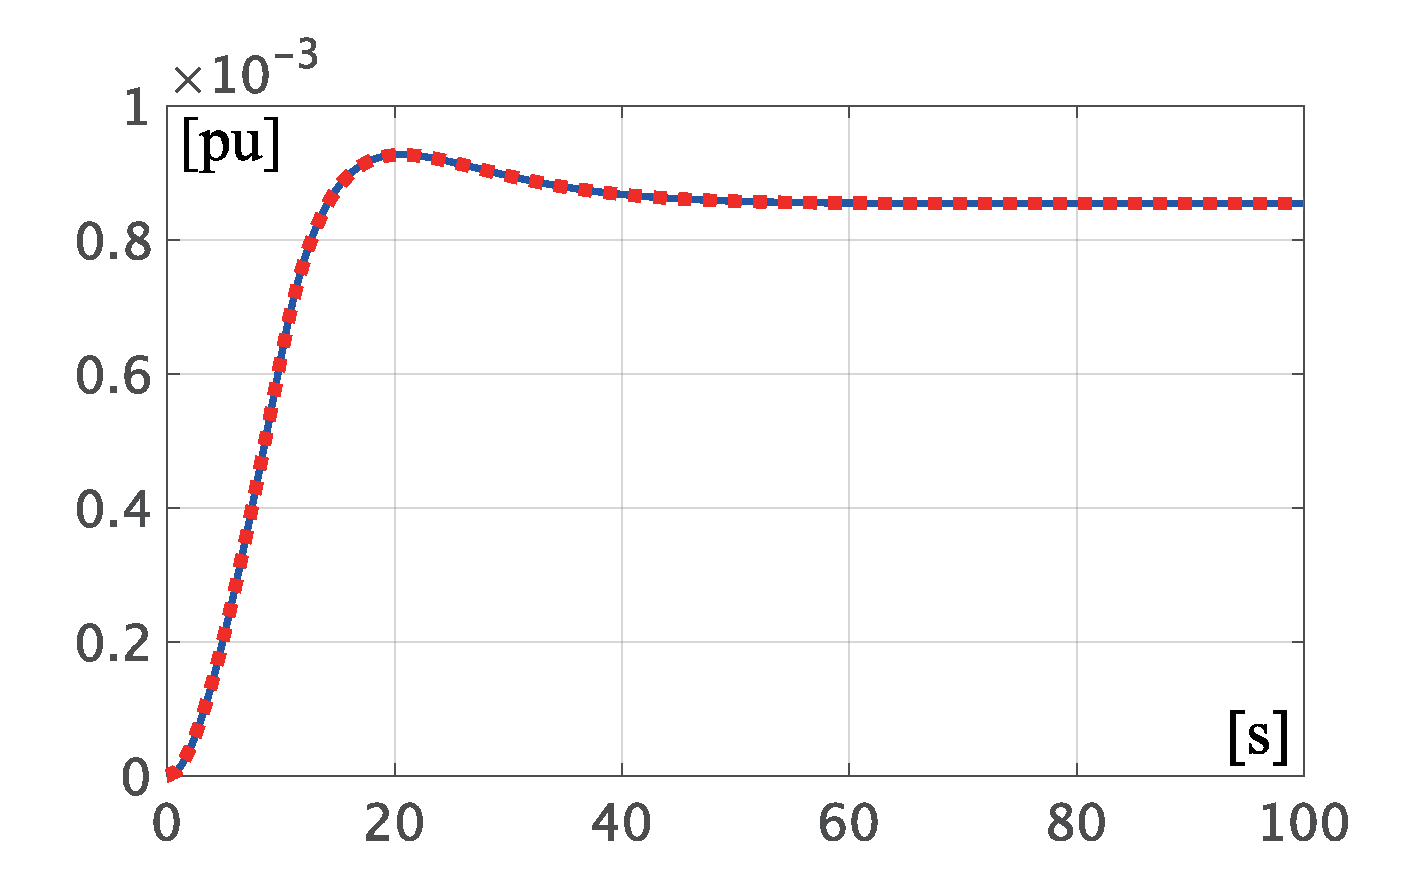
\includegraphics[width = 1.0\linewidth]{figs/P1pl}
    \subcaption{If the resistance is reduced by 1\%}
  \end{minipage}
  \medskip
  \caption{\textbf{Time response of angular frequency deviation to load change}
  \\ \centering(Steady-state state of Table \ref{table:pflow1}, line type is
  the same as Figure \ref{fig:P13ini}.)}
  \label{fig:P1load}
  }
\medskip
\end{figure}

\begin{figure}[t]
  \centering
  {
  \begin{minipage}{0.49\linewidth}
    \centering
    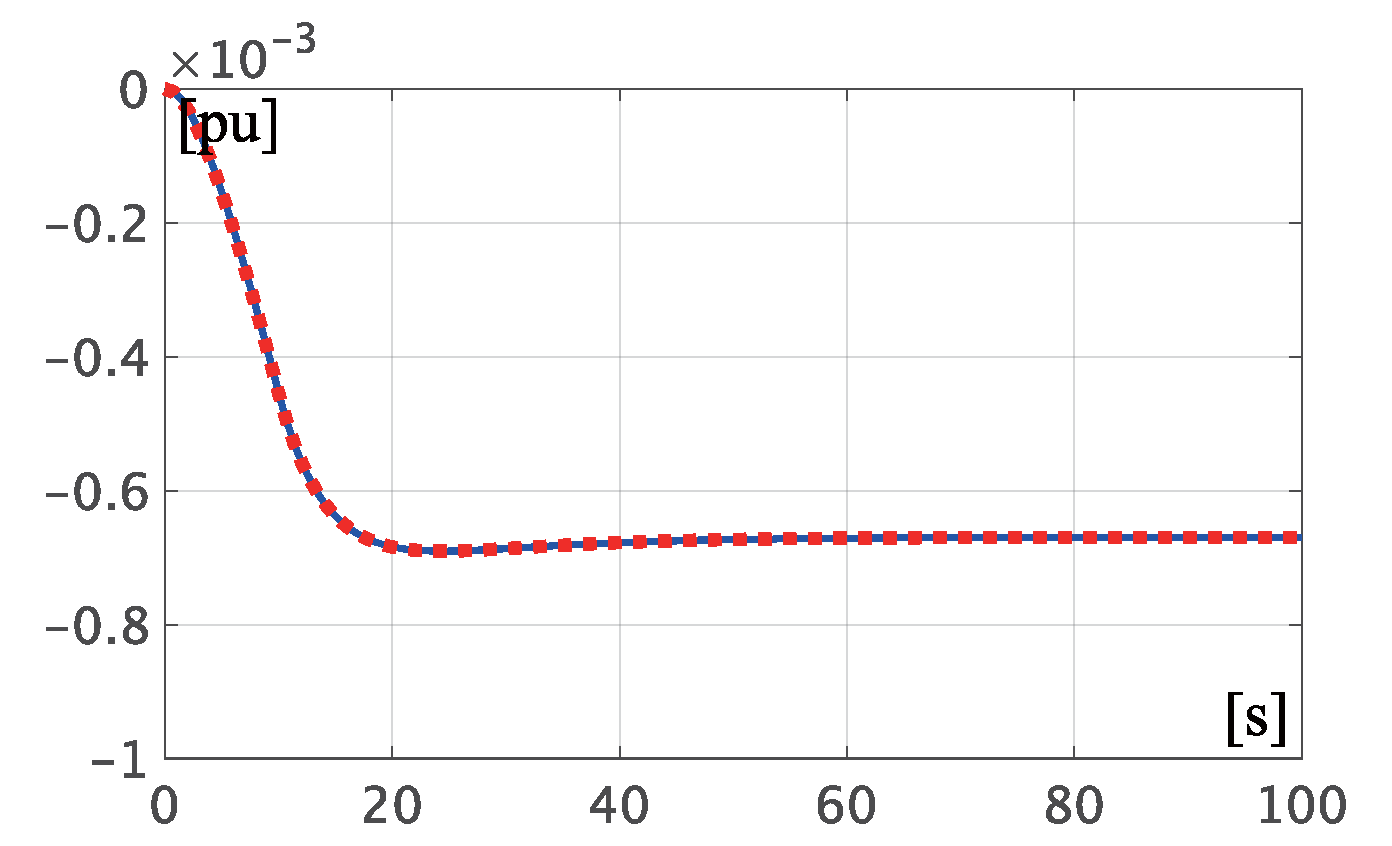
\includegraphics[width = 1.0\linewidth]{figs/P3mi}
    \subcaption{If resistance is increased by 1\%}
  \end{minipage}
  \begin{minipage}{0.49\linewidth}
    \centering
    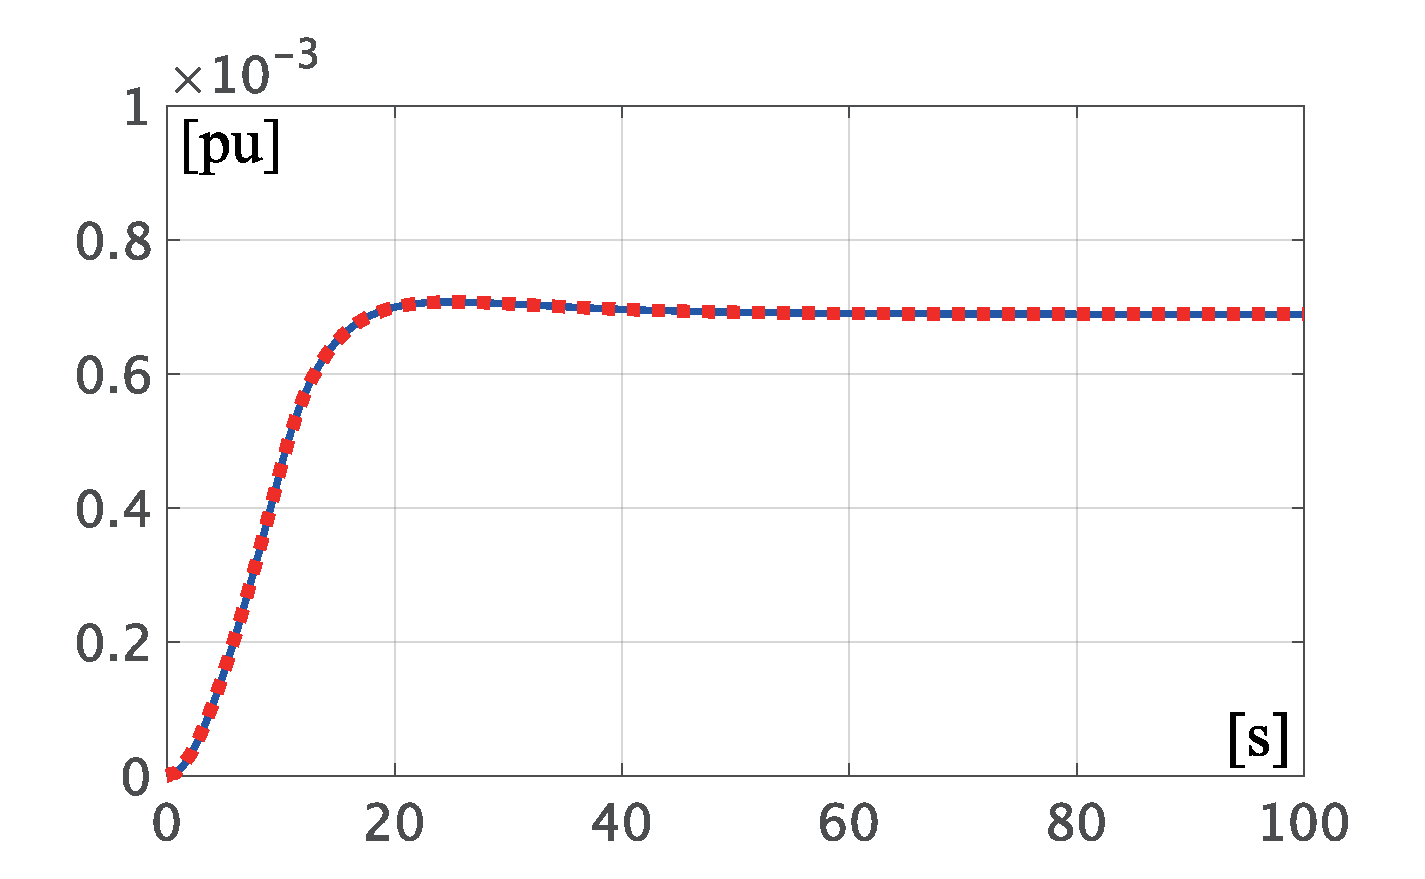
\includegraphics[width = 1.0\linewidth]{figs/P3pl}
    \subcaption{If the resistance is reduced by 1\%}
  \end{minipage}
  \medskip
  \caption{\textbf{Time response of angular frequency deviation to changes in load}
  \\ \centering(Steady-state of Table \ref{table:pflow2}, line type is the same
  as Figure \ref{fig:P13ini}.)}
  \label{fig:P3load}
  }
\medskip
\end{figure}
In Example \ref{ex:loadpv}, unlike the result in Example \ref{ex:inires}, the
generator's frequency deviation has a non-zero steady-state value. In order to
make this frequency deviation zero, it is necessary to adjust the mechanical
input or excitation input of the generator group appropriately. On the other
hand, to make the steady-state value of the frequency deviation zero, frequency
control is generally performed by a control algorithm that adjusts the
mechanical input of the generator group to balance the demand and supply of
active power. However, it is practically difficult to accurately measure the
changes in all loads. Therefore, feedback control that automatically searches
for the value of the mechanical input that achieves the demand-supply balance
through control operations based on an integrator is necessary. The details of
this are described later in Sections \ref{sec:agcover} and \ref{sec:mathnpas}.

\subsection{Response to ground fault}\label{sec:fault}

\smallskip
\subsubsection{What is ground fault?}

When an electric circuit comes into contact with the ground due to contact with
an object or lightning strike, a phenomenon called \textbf{ground fault} occurs,
and a large current flows into the ground. Ground fault detection devices
quickly operate in power systems to detect the occurrence of ground fault and
block the ground fault current. If the ground fault current is removed and the
blocking is released, the power system operation before the occurrence of ground
fault can be restored.

The time required to detect and remove ground fault is generally about 70 [ms].
During this time, the ground fault current flowing into the ground can cause
severe disturbances to the power system operation. Note that the disturbance due
to ground fault is not modeled as an external input, but is modeled as a
"switching to a different power system model during the time when the ground
fault is still present."

\smallskip
\subsubsection{Formulation of bus bar ground fault}

Bus bar ground faults discussed in this book are modeled assuming that the
voltage phasor of the bus is constrained to zero during the time the fault
persists. Without losing generality, we explain it for the case where a fault
occurs on bus bar $1$ of a power system model consisting of $N$ bus bars.
Additionally, we assume that the fault occurs at time $0$ and persists until
time $t_0$. Under these conditions, the power flow state in Equation
\ref{eq:pfconIV} satisfies the algebraic equation of the normal operating state
in Equation \ref{eq:ohmY2} for $t < 0$ and $t \geq t_0$. However, for the time
period when the fault persists, $t \in [0, t_0)$, the power flow state must
satisfy the algebraic equation in Equation \ref{eq:ohmY2f}, which excludes the
equation related to the current phasor of the faulted bus $\bm{I}_{1}(t)$, and
the constraint condition on the voltage phasor of the faulted bus:

\begin{subequations}\label{eq:ohmY2f}
 \begin{align}
\mat{
  \bm{I}_2(t)\\
  \vdots\\
  \bm{I}_{N}(t)
}
 =
\mat{
  \bm{Y}_{22} & \cdots & \bm{Y}_{2N}\\
  \vdots & \ddots & \vdots\\
  \bm{Y}_{N2} & \cdots & \bm{Y}_{NN}
}
\mat{
  \bm{V}_2(t)\\
  \vdots\\
  \bm{V}_{N}(t)
}
\end{align}
and the constraint condition on the voltage phase of the faulted bus:
\begin{align}
|\bm{V}_{1}(t)| = 0
\end{align}
\end{subequations}

Note that for buses and time periods where a ground fault has not occurred, the
voltage and current phasors follow the differential or algebraic equations that
represent each equipment's model. This is the same as during normal operation.
Therefore, in numerical simulations, it is necessary to switch between the
following two models:
\begin{itemize}
  \item During periods where a ground fault has not occurred, the normal power
  system model is used.
  \item During periods where a ground fault is ongoing, the power system model
  is used with the affected bus and its connected equipment and transmission
  lines removed.
\end{itemize}

The current phasor $\bm{I}{1}(t)$ flowing from device $1$ to bus $1$ during a
ground fault is determined by the dynamic characteristics of the device.
Specifically, if the device is a generator, then its internal state evolves over
time according to following differential equations for $t\in [0, t_0)$, where
$|\bm{V}{1}(t)|$ is set to 0. 

\begin{equation}\label{eq:gendynVIfN}
  \simode{
    \dot{\delta}_1&= \omega_0  \Delta \omega_1\\
    M_1   \Delta \dot{\omega}_1 &= 
    - D_1 \Delta\omega_1  
    +P_{{\rm mech}1} 
    \\
    \taud_1 \dot{E}_1 & = 
    - \tfrac{ \Xs_1 }{ \Xt_1 }E_1
    + V_{{\rm field}1}
  }
\end{equation}

In this case, current phasor $\bm{I}_{1}(t)$ is given with the following as an
output of generators:

\begin{align*}%\label{eq:IoutfN}
|\bm{I}_1(t)|=\frac{E_1 (t)}{ \Xt_1 }
,\qquad
\angle \bm{I}_1 (t) = \delta_1 (t) - \frac{\pi}{2}
\end{align*}

On the other hand, if device $1$ is modeled as a constant impedance load,
then $|\bm{I}{1}(t)|$ is also zero since $|\bm{V}{1}(t)|$ is zero as given by
Eq. \eqref{eq:cimp}. For other load models, the situation is generally similar,
except that for constant power loads, $|\bm{I}{1}(t)|$ becomes infinite, so
numerical instability must be taken into account in simulations. Note that the
ground fault current phasor flowing from bus $1$ to ground can be expressed as

\[
  \bm{I}_{1}'(t) := \bm{I}_{1}(t) - \sum_{j=2}^{N} \bm{Y}_{1j} \bm{V}_{j}(t),\qquad
  t \in [0, t_0)
\]
where $N$ is the number of buses.

The value of the ground fault current phasor does not need to be calculated for
the purpose of running numerical simulations of power system models. On the
other hand, when a generator is connected to the ground fault bus, it is
important to calculate the value of the generator's internal state at the time
$t_0$ when the ground fault is cleared, so it is necessary to solve the
differential equations in Equation \ref{eq:gendynVIfN}. For the initial internal
states of each generator at the time of the ground fault occurrence, arbitrary
values can be set for any flow state. In this book, appropriate values obtained
as a result of the power flow calculation for a steady-state flow condition are
used. Note that at the time of occurrence and clearance of the ground fault, the
internal states of each generator are continuous, but the voltage and current
phasors of each bus change discontinuously.

The calculation of the time response for bus-ground faults can be summarized in
the following steps:

\medskip
\begin{breakbox}
\begin{itemize}
  \item[(a)] Set the variable values at the steady-state condition obtained from
  the power flow calculation as the initial values of the internal states of each
  generator. 
  \item[(b)] Calculate the time evolution using the power system model that
  excludes the faulted bus and the devices and transmission lines connected to it,
  for the time interval $t \in [0, t_0)$, where the fault persists.
  \item[(c)] If a generator is connected to the faulted bus, set the bus voltage
  phase to zero for $t \in [0, t_0)$, and calculate the time evolution of its
  internal state.
  \item[(d)] Set the values of the internal states of each generator at time
  $t_0$, and calculate the time evolution of the system after the fault is cleared
  using the usual power system model with all devices connected. 
\end{itemize}
\end{breakbox}
\medskip

Let us calculate the time response for bus-ground faults using these steps.

\begin{example}[Time response of power system model to bus bar ground
fault]\label{ex:busflt}

In the same setting as Examples \ref{ex:inires} and \ref{ex:loadpv}, let us
calculate the time response of the frequency deviation of the bus due to ground
fault. Specifically, we set the two steady-state power flow states obtained by
power flow calculation as initial values and calculate the time response when a
ground fault occurs at bus 1. For comparison, we consider two cases where the
time until the fault is cleared is 50 [ms] and 100 [ms], respectively.

The calculation results are shown in Figures \ref{fig:P1fault} and
\ref{fig:P3fault}.  The solid blue line represents the frequency deviation of
generator 1, and the dashed red line represents the frequency deviation of
generator 3.  From Figure \ref{fig:P1fault}, it can be seen that the frequency
oscillation of generator 3 is large in the steady-state power flow state shown
in Table \ref{table:pflow1}.  In particular, a larger oscillation occurs when
the duration of the ground fault is 100 [ms].  The reason why the oscillation of
generator 3 is larger is that, as shown in Table \ref{table:genparams}, the
inertia constant of generator 1 is large at 100 [s], while that of generator 3
is small at 12 [s].  In other words, the oscillation of the generator with
larger inertia causes the larger oscillation of the generator with smaller
inertia.

On the other hand, it can be seen from Figure \ref{fig:P3fault} that the frequency
oscillation for the same ground fault is small in the steady-state power flow
state shown in Table \ref{table:pflow2}. This is because in the steady-state
power flow state of Table \ref{table:pflow1}, generator 3 with small inertia
supplied most of the active power consumed by the load, while in the
steady-state power flow state of Table \ref{table:pflow2}, generator 1 with
large inertia supplied most of the active power. In general, synchronous
generators have the characteristic that their sensitivity to disturbances
increases as the supplied power approaches its maximum value. In the
steady-state power flow state of Table \ref{table:pflow2}, the stability of
generator 3 with small inertia is relatively high, so the sensitivity of the
frequency deviation to the ground fault is low.
\end{example}

\begin{figure}[t]
  \centering
  {
  \begin{minipage}{0.49\linewidth}
    \centering
    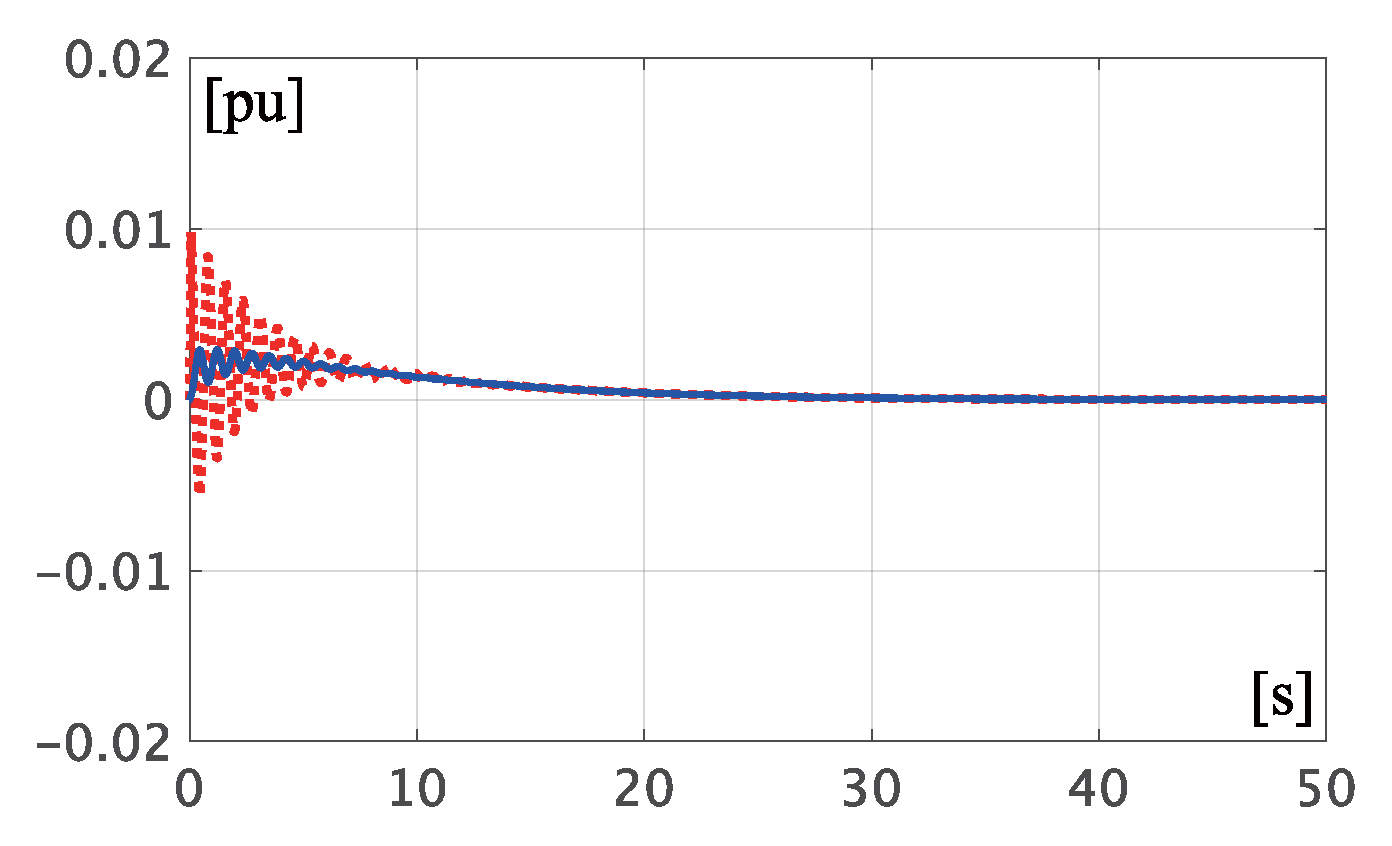
\includegraphics[width = 1.0\linewidth]{figs/50mP1}
    \subcaption{Ground fault at 50~[ms]}
  \end{minipage}
  \begin{minipage}{0.49\linewidth}
    \centering
    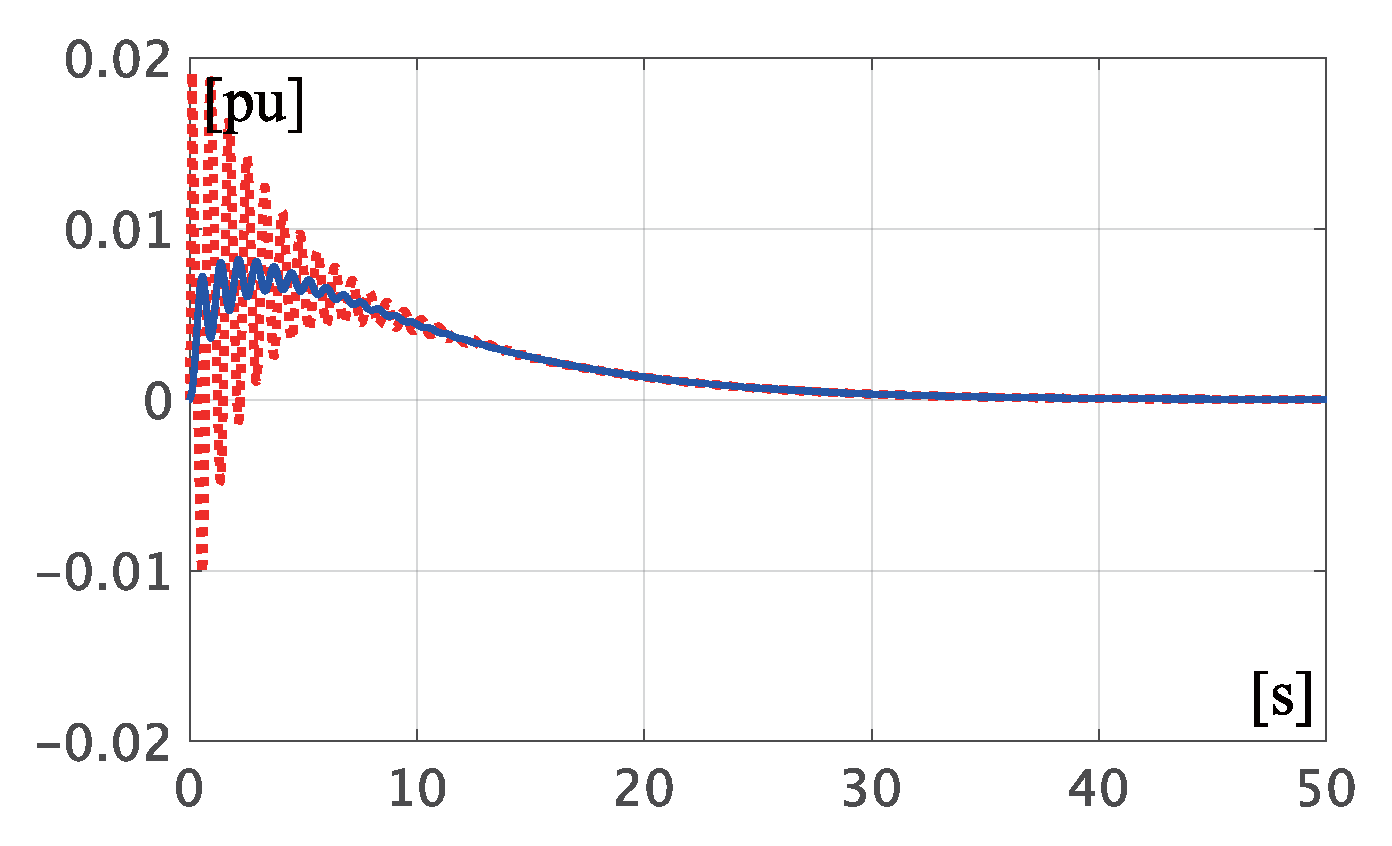
\includegraphics[width = 1.0\linewidth]{figs/100mP1}
    \subcaption{Ground fault at 100~[ms]}
  \end{minipage}
  \medskip
  \caption{\textbf{Time response of angular frequency deviation to ground fault}
  \\ \centering (Steady-state of \ref{table:pflow1}, line type is the same as \ref{fig:P13ini})}
  \label{fig:P1fault}
  }
\medskip
\end{figure}

\begin{figure}[t]
  \centering
  {
  \begin{minipage}{0.49\linewidth}
    \centering
    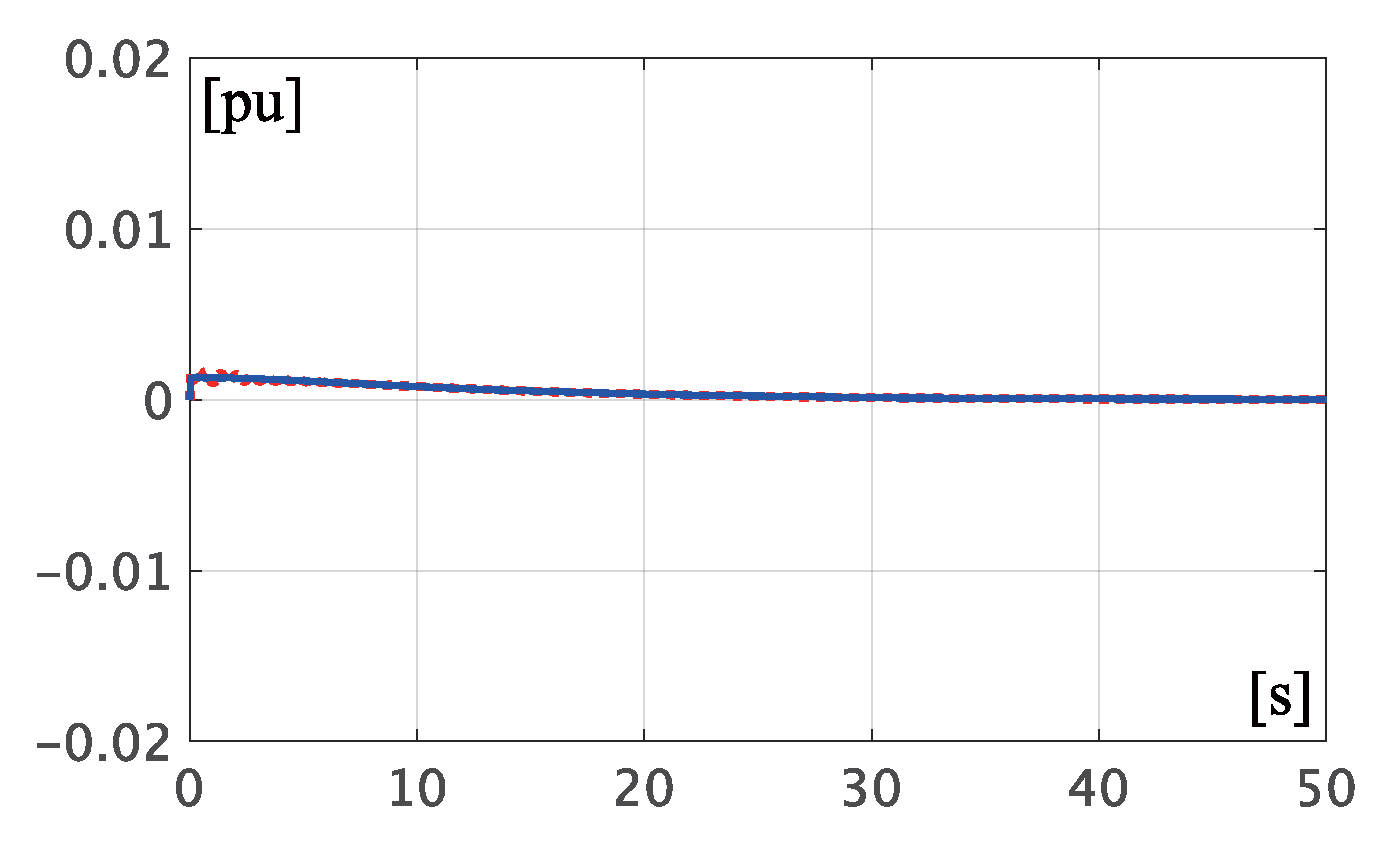
\includegraphics[width = 1.0\linewidth]{figs/50mP3}
    \subcaption{ Ground fault at 50~[ms]\label{fig:P3faulta}}
  \end{minipage}
  \begin{minipage}{0.49\linewidth}
    \centering
    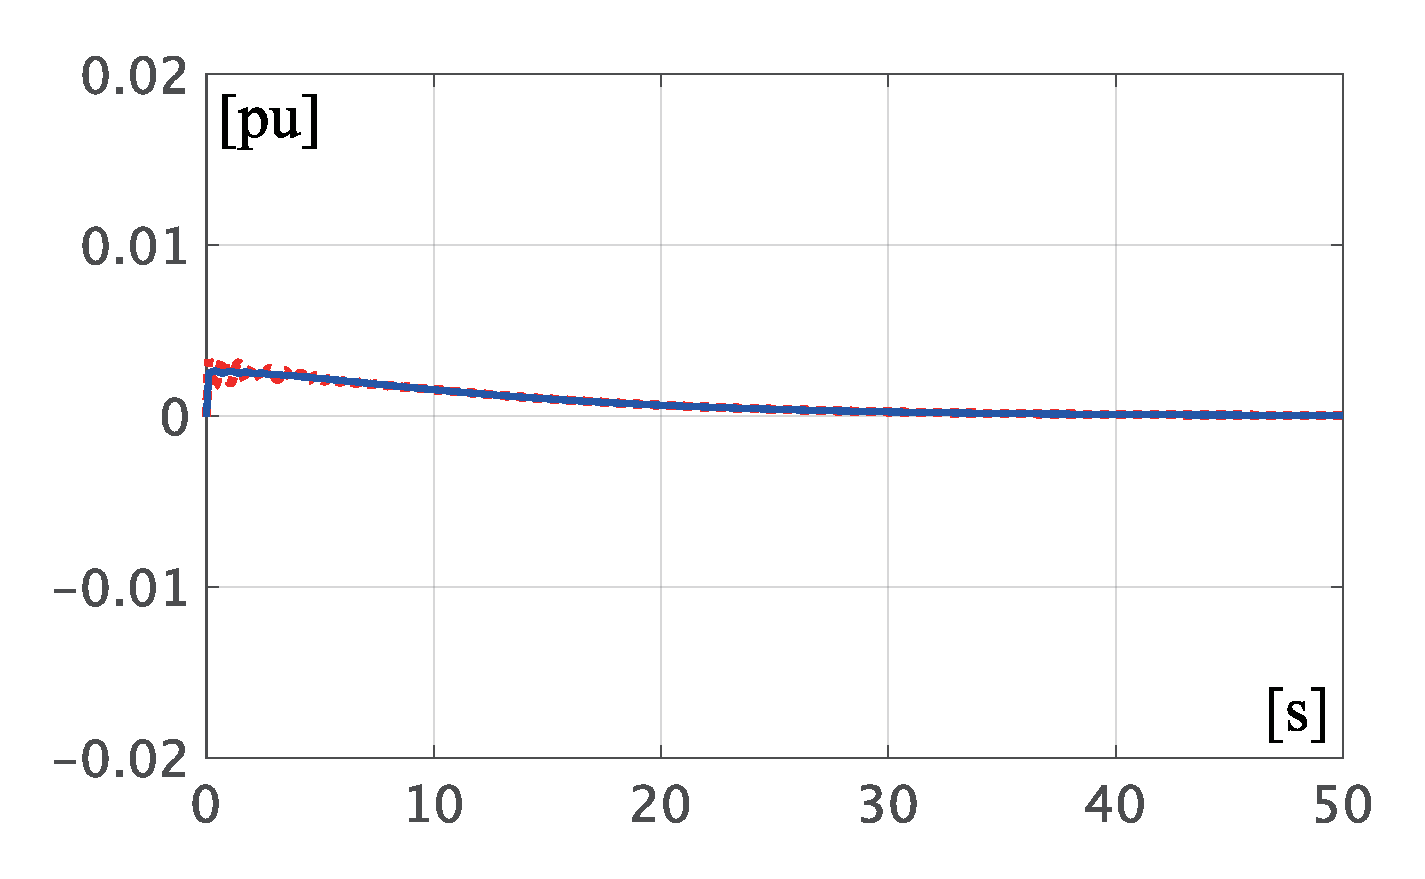
\includegraphics[width = 1.0\linewidth]{figs/100mP3}
    \subcaption{Ground fault at 100~[ms]}
  \end{minipage}
  \medskip
  \caption{\textbf{Time response of angular frequency deviation to ground fault}
  \\ \centering (Steady-state of \ref{table:pflow2}, line type is the same as \ref{fig:P13ini})}
  \label{fig:P3fault}
  }
\medskip
\end{figure}

From Example \ref{ex:busflt}, it can be seen that the stability of the power
system model for ground faults varies depending on the steady-state power flow
condition (equilibrium point). In particular, in Example \ref{ex:pf3bus}, the
steady-state power flow condition in Table \ref{table:pflow1} was superior from
the perspective of transmission loss, while in Example \ref{ex:busflt}, the
steady-state power flow condition in Table \ref{table:pflow2} was found to be
superior in terms of system stability with respect to ground faults. These
examples suggest the importance of exploring desirable equilibrium points,
taking into account trade-offs between factors such as economic efficiency and
stability.

It should be noted that ground faults may occur at various locations and not
only on specific buses or transmission lines, so it is necessary to improve the
overall stability of the power system in a meaningful way. Control mechanisms
for this purpose are explained in Sections \ref{sec:transcont} and
\ref{sec:retrofit}.

Furthermore, from the simulation results of Examples \ref{ex:inires} to
\ref{ex:busflt}, it can be observed that when the internal state settles into a
steady state without diverging, "all generator frequency deviations have
converged to the same value." Similar results are also observed in Example
\ref{ex:Kronode}. This synchronization of frequency in the steady-state power
flow condition is a universal phenomenon in power system models. Frequency
control, which will be discussed in Sections \ref{sec:agcover} and
\ref{sec:mathnpas}, is based on the assumption that the frequency will
automatically synchronize in the steady-state power flow condition, and control
algorithms are constructed accordingly.

\section{Synchronization of bus bar voltage in a steady power flow distribution\advanced}\label{sec:phsync}

In this section, we mathematically investigate the frequency synchronization
phenomenon observed in Section \ref{sec:numsimtr} from the perspective of the
graph structure of the power transmission network. Based on the results of
Theorem \ref{thm:outst}, we introduce the following definition.

\begin{definition}[Synchronization of the steady power flow distribution and bus
bar voltage] \label{def:sync}

Consider the power system model in which the devices are coupled by the
simultaneous equations of Equation \ref{eq:PQVgen}. For all buses $i$, if the
following hold for all $t\geq0$, the power system is said to be in a
\textbf{steady-state power flow}\index{steady-state power flow}.

\begin{equation}\label{eq:stapfs}
  \frac{dP_i}{dt}(t)=0
  ,\quad
  \frac{dQ_i}{dt}(t)=0
  ,\quad
  \frac{d|\bm{V}_i|}{dt}(t)=0
  ,\quad
  \frac{d^2 \angle \bm{V}_i }{dt^2}(t)=0
\end{equation}

\footnote{
Please note that the mathematical definition of this “steady power flow distribution” is unique to this book and is not typically used in electrical power system engineering.
}

Moreover, if the power system is in a steady-state power flow and Equation
\ref{eq:defsyn} holds, the buses $i$ and $j$ are said to be
\textbf{synchronized}\index{synchronization} in the steady-state power flow.

\begin{equation}\label{eq:defsyn}
  \frac{d \angle \bm{V}_i}{dt}(t) =  \frac{d \angle \bm{V}_j}{dt}(t)
\end{equation}
\end{definition}
As stated in Theorem \ref{thm:outst}, the validity of Equation \ref{eq:stapfs}
for the generator bus is equivalent to the internal state of the generator and
the external input being in steady state. Moreover, if any selected
pair of buses $(i,j)$ are in synchronized in the sense of Definition
\ref{def:sync}, it can be concluded that the angular frequency deviation of all
generators converges to the same value. Note that the validity of Equation
\ref{eq:stapfs} for any bus applies to the current phase $\bm{I}_i$.

\begin{equation*}
  \frac{d|\bm{I}_i|}{dt}(t)=0
  ,\qquad
  \frac{d^2 \angle \bm{I}_i }{dt^2}(t)=0
  ,\qquad
  \frac{d \angle \bm{I}_i }{dt}(t) = \frac{d \angle \bm{V}_i }{dt} (t)
\end{equation*}

is true for current phasor $\bm{I}_i$.
This can be easily confirmed since:

\begin{align*}
|P_i(t) + \bm{j} Q_i(t)| = |\bm{V}_i(t)| |\bm{I}_i(t)|
,\qquad
\angle(P_i(t) + \bm{j} Q_i(t)) = \angle \bm{V}_i(t) - \angle \bm{I}_i(t)
\end{align*}

A set of adjacent bus bars connected to the bus bar $i$ with a transmission line is expressed as $\mathcal{N}_i$. 
In other words:

\begin{align*}
\mathcal{N}_i:=
\left\{
j : \bm{Y}_{ij} \neq 0,\quad j \neq i
\right\}
\end{align*}

The number of adjacent bus bars connected to the bus bar $i$ with a transmission line is $|\mathcal{N}_i|$.
This is called "\textbf{ degree} of bus bar $i$ is $|\mathcal{N}_i|$".
We can use the following expression assuming that the electrical power system model is in the steady power flow distribution, 

\begin{align*}
\angle \bm{V}_i (t) = \Omega_i t +\phi_i
\end{align*}

However, $\Omega_i$ and $\phi_i$ are constant. 
At this time, electric power balance equation for bus bar $i$ in Equation \ref{eq:PQVgen} is:

\[
P_i + \bm{j} Q_i = \sum_{j=1}^N \overline{\bm{Y}}_{ij} |\bm{V}_i| |\bm{V}_j|
e^{\bm{j} \left\{ ( \Omega_i - \Omega_j )t + \phi_i -\phi_j \right\}}
\]

If we assume a steady power flow distribution, the absolute value of the active power, reactive power, and bus bar voltage phasor provided to the bus bar $i$ are all constants.
If these are expressed as $P_i^{\star}$, $Q_i^{\star}$, and $|\bm{V}_i^{\star}|$, this electric power balance equation can be rewritten as:

\begin{align}\label{eq:sumcirc}
\underbrace{
\frac{1}{|\mathcal{N}_i|}\sum_{j \in \mathcal{N}_i } 
r_{ij}
e^{\bm{j} 
\left(
\Omega_{ij}t + 
\Phi_{ij}
\right) }
}_{\bm{C}_i (t)}
= \bm{z}_i
\end{align}

However, the frequency difference of the voltage phasor for bus bars $i$ and $j$ is expressed as:

\[
\Omega_{ij}:=\Omega_{i}-\Omega_{j}
\]

$r_{ij}$, $\Phi_{ij}$, and $\bm{z}_i$ are all constants, and defined by:

\begin{align*}
r_{ij} &:=|\bm{V}_i^{\star}| |\bm{V}_j^{\star}| |\bm{Y}_{ij}|, \qquad
\Phi_{ij} := \phi_i - \phi_j - \angle \bm{Y}_{ij},
\\
\bm{z}_i &:=  \tfrac{
\left\{
P_i^{\star} - \real[\bm{Y}_{ii}] |\bm{V}_i^{\star}|^2
+ \bm{j}
\left(
Q_i^{\star} + \imag [\bm{Y}_{ii}] |\bm{V}_i^{\star}|^2
\right)
\right\}
}
{|\mathcal{N}_i|}
\end{align*}

Below, let us think about $\Omega_{ij}$ being 0 for all $j\in \mathcal{N}_i$ as an equation that expresses the synchronicity with adjacent bus bars from Equation \ref{eq:sumcirc};
in other words, let us think about deriving: 

\begin{align}\label{eq:alloms}
\Omega_i = \Omega_{j} 
,\qquad 
\forall j\in \mathcal{N}_i
\end{align}

Here, Equation \ref{eq:sumcirc} expresses that "the center of gravity $\bm{C}_i (t)$ of $|\mathcal{N}_i|$ points that move at a constant velocity on the circumference of a circle with the radius of $r_{ij}$ with the origin as the center with the initial phase of $\Phi_{ij}$ and the angular velocity of $\Omega_{ij}$ is invariable on a point $\bm{z}_i$ on a complex plane".
Figure \ref{fig:centerg} shows the relationship when bus bar $1$ is connected to bus bar $2$ and bus bar $3$. Focusing on this fact, the following result can be derived.

\begin{figure}[t]
\centering
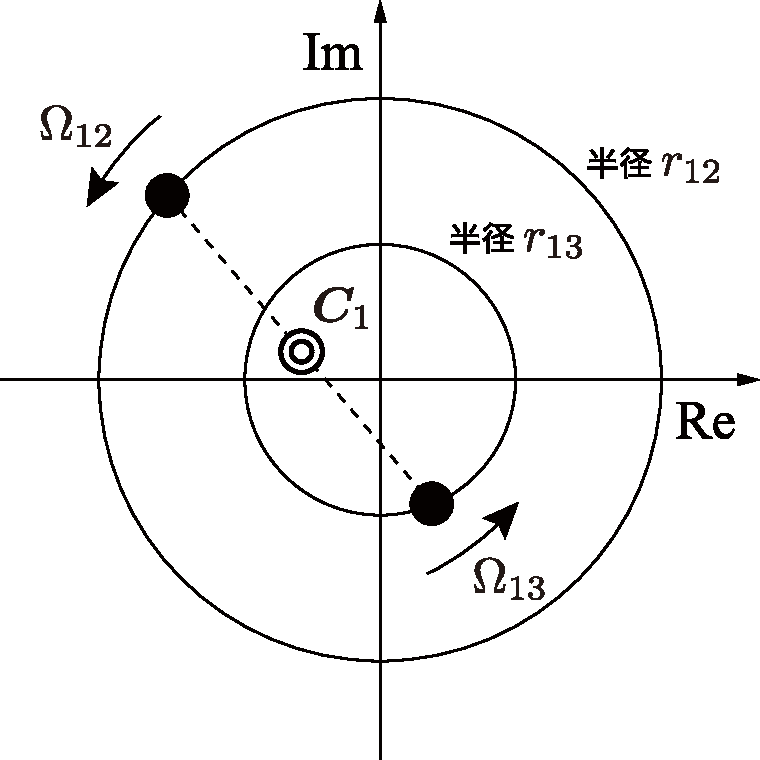
\includegraphics[width = .4\linewidth]{figs/centerg}
\medskip
\caption{\textbf{When bus bar 1 is connected to bus bars 2 and 3}}
\label{fig:centerg}
\medskip
\end{figure}


\begin{lemma}[Synchronization of bus bars derived from the balance equation of electric power]
\label{lem:sumc2}

Let us consider $\bm{C}_i (t)$ of Equation \ref{eq:sumcirc} for real constants $r_{ij}$, $\Omega_i$, $\Omega_j$, and $\Phi_{ij}$, where $r_{ij}>0$.
At this time, if $|\mathcal{N}_i|=1$, $\bm{C}_i (t)$ being a constant that is not dependent on $t$ is equivalent to Equation \ref{eq:alloms}.
In addition, if $|\mathcal{N}_i|=2$, $\bm{C}_i (t)$ being a constant that is not dependent on $t$ is equivalent to Equation \ref{eq:alloms} being true, or to:

\begin{align}\label{eq:N2sing}
\Omega_{j_1} = \Omega_{j_2}
,\qquad
r_{i j_1} = r_{i j_2}
,\qquad
|\Phi_{i j_1}-\Phi_{i j_2}| = \pi
\end{align}

where $\mathcal{N}_i = \{j_1,j_2\}$.
Furthermore, if $|\mathcal{N}_i|=3$, $\bm{C}_i (t)$ being a constant that is not dependent on $t$ is equivalent to Equation \ref{eq:alloms} being true,
or Equation \ref{eq:N2sing} being true for $j_3 \in \mathcal{N}_i$ satisfying $\Omega_{i} = \Omega_{j_3}$, where $ \mathcal{N}_i \setminus \{j_3\}=\{j_1,j_2\}$.

\begin{align}\label{eq:threeoms}
\Omega_{j_1} = \Omega_{j_2}= \Omega_{j_2}
,\qquad 
\sum_{j\in \mathcal{N}_i} 
r_{ij} e^{\bm{j} \Phi_{ij}}=0
\end{align}
\end{lemma}

\begin{proof}
\red{Translated with DeepL}
By applying the complementary problem\ref{lem:sumc} at the end of the chapter, we can show the facts for the cases $|\mathcal{N}_i|=1$ and $|\mathcal{N}_i|=2$.
Thus, in the following we consider the case $|\mathcal{N}_i|=3$.
For simplicity of notation, let $j \in\{1,2,3\}$ and denote $r_{ij}$, $\Phi_{ij}$, $\Omega_i$ and $\bm{C}_i$ as $r_{j}$, $\Phi_{j}$, $\Omega_0$ and $\bm{C}_0$ respectively.
First, let's consider the following case,
\begin{align}\label{eq:omjeq}
\Omega_j \neq \Omega_0
,\qquad \forall j \in \{1,2,3\}
\end{align}
From the complement \ref{lem:sumc}, when the formula\ref{eq:omjeq} holds, the formula\ref{eq:sumcirc} is equivalent to:
\begin{align*}
\Omega_1 = \Omega_2 = \Omega_3,\qquad
\sum_{j=1}^3 
r_j e^{\bm{j} \Phi_j}=0
\end{align*}
This implies that the expression \ref{eq:threesoms}
%しかしながら,$\Omega_1 = \Omega_2 = \Omega_3$である場合には,$|\mathcal{N}_i|=1$のときと同様にして,$\bm{C}_i (t)$が$t$に依らない定数であることと式\ref{eq:alloms}が等価であることが導かれる。
%これは式\ref{eq:omjeq}に矛盾する。

Next, consider the case where the expression \ref{eq:omjeq} does not hold, i.e., where $\Omega_0=\Omega_j$ for some $j\in\{1,2,3\}$.
In particular, consider the case where $\Omega_0=\Omega_3$ without loss of generality from symmetry with respect to $j$.
In this case
\begin{align*}
\bm{C}_0 (t) = \frac{1}{3} \left\{
r_3 e^{\bm{j} \Phi_3}
+
\sum_{j=1}^2
r_{j}
e^{\bm{j} 
\left\{
(\Omega_0 - \Omega_j)t + 
\Phi_{j}
\right\} }
\right\}
\end{align*}
であることから,$t$に関する不変性は,$|\mathcal{N}_i|=2$の場合と同様に議論できる。
したがって,$\bm{C}_0 (t)$が$t$に依らない定数であることは,式\ref{eq:alloms}または
\begin{align*}
\Omega_{1} = \Omega_{2}
,\qquad
r_{1} = r_{2}
,\qquad
|\Phi_{1}-\Phi_{2}| = \pi
\end{align*}
と等価である。
以上より題意が示される。
\end{proof}

Lemma \ref{lem:sumc2} shows that when the degree of the bus bar of interest is 1; in other words, for end-point bus bars such as Figure \ref{fig:bussync}(a), bus bars adjacent to such bus bars synchronize.
In addition, if the degree of the bus bar of interest (the node shown with a thick line) is 2; in other words, for bus bars in a chain such as Figure \ref{fig:bussync}(b), at least on bus bar on each side, are synchronized.
Furthermore, when the degree of the bus bar of interest is 3; meaning, a bus bar of a node is connected with three transmission lines as in Figure \ref{fig:bussync}(c), at least one adjacent bus bar synchronizes with the bus bar of interest.
This means that there is no situation where only three arbitrarily chosen bus bars are synchronized and one remaining bus bar is not synchronized, or no set of bus bars is synchronized.

\begin{figure}[t]
  \centering
  {
  \begin{minipage}{0.24\linewidth}
    \centering
    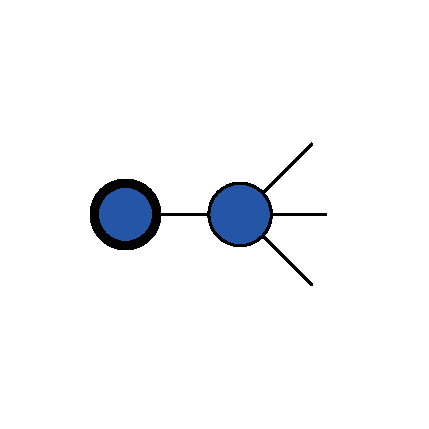
\includegraphics[width = .85\linewidth]{figs/1degbus}
    \subcaption{ 次数1の母線}
    \label{fig:N1} 
  \end{minipage}
  \begin{minipage}{0.24\linewidth}
    \centering
    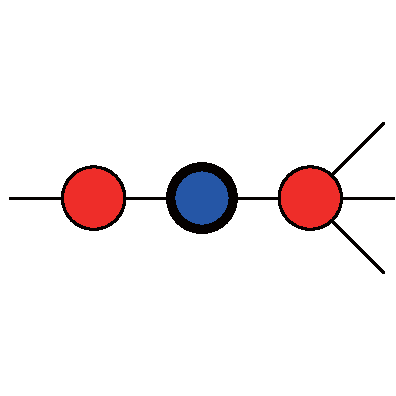
\includegraphics[width = .85\linewidth]{figs/2degbus}
    \subcaption{ 次数2の母線}
  \end{minipage}
  \label{fig:N2}
  \begin{minipage}{0.48\linewidth}
    \centering
    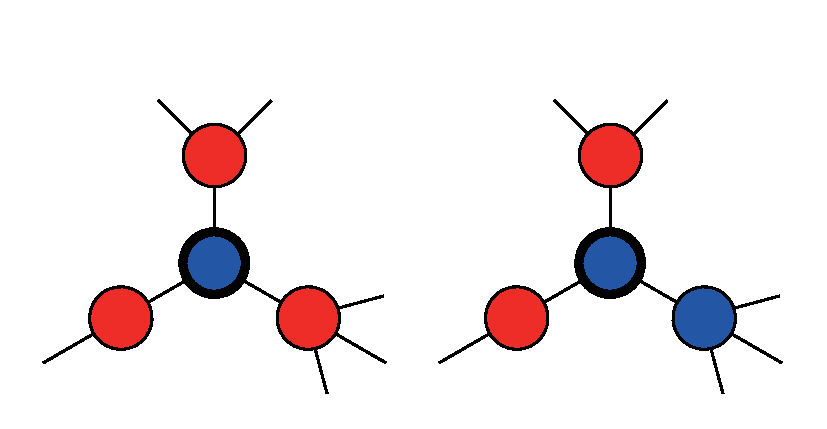
\includegraphics[width = .85\linewidth]{figs/3degbus}
    \subcaption{ 次数3の母線 }
  \end{minipage}
  \medskip
  \caption{\textbf{母線の次数に応じた隣接母線との同期}}
  \label{fig:bussync}
  }
\medskip
\end{figure}
When the degree of the bus bar of interest is four or higher, the same analysis can be performed.
However, since the obtained conditions could be a higher-order equation related to $\Omega_i$ and $\Omega_j$, or there are multiple combinations where only some adjacent bus bars that are arbitrarily selected synchronize, describing the equivalent conditions for synchronization is usually cumbersome.
However, for the bus bar of interest $i$ and $|\mathcal{N}_i|$ adjacent bus bars, if some of the $|\mathcal{N}_i |-1$ adjacent bus bars synchronize with the bus bar $i$, the remaining one adjacent bus bar usually synchronizes. 

By combining conditions with the degree of three or less shown in lemma \ref{lem:sumc2}, even when a bus bar with degree of four or more is included in the power grid, all bus bars could be synchronized.
For example, the next fact can be shown.

\begin{theorem}[Synchronization of bus bars in a tree-structured power grid]
\label{thm:tree}
With simultaneous equations of Equation \ref{eq:PQVgen}, let us consider an electrical power system model in which a group of equipment is connected.
When the graph of the power grid has a tree structure, all bus bars are synchronized under a steady power flow distribution.
%\footnote{
%グラフ理論において,連結であり閉路をもたないグラフは\textbf{木}(tree)と呼ばれる。
%}
\end{theorem}

\begin{proof}
\red{Translated with DeepL}
Note the bus bar at the endpoint indicated by the bold line in Figure \ref{fig:treepr}(a).
Since the order of the bus bar is 1, the adjacent bus bars are synchronous with the bus bars of the endpoints.
Next, if the bus bar next to the endpoint is in the chain path, the degree of the bus bar is 2, so at least both of its adjacent bus bars are synchronized.
By repeating this process, as in Figure \ref{fig:treepr}(a), synchronization of all the bus bars is shown in the chain path connecting the endpoint and the bus bars of nodes of degree 3 or more.

Similarly, since all the bus bars in a node of degree 3 or more from another endpoint are synchronous, we see that all the bus bars in all chain paths connected to the bus bar in the node indicated by the bold line, as in Figure \ref{fig:treepr}, are all synchronous.
Repeating this argument, it can be shown that all the bus bars composing the tree are synchronous.
\end{proof}


\begin{figure}[t]
  \centering
  {
  \begin{minipage}{0.40\linewidth}
    \centering
    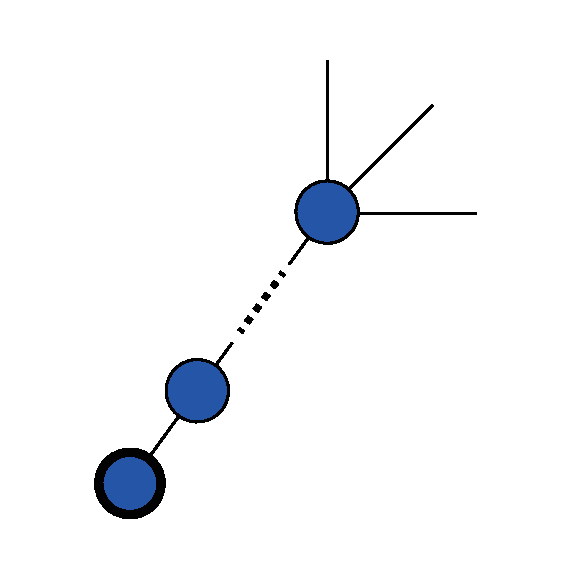
\includegraphics[width = .50\linewidth]{figs/treesub}
    \subcaption{ }
  \end{minipage}
  \begin{minipage}{0.40\linewidth}
    \centering
    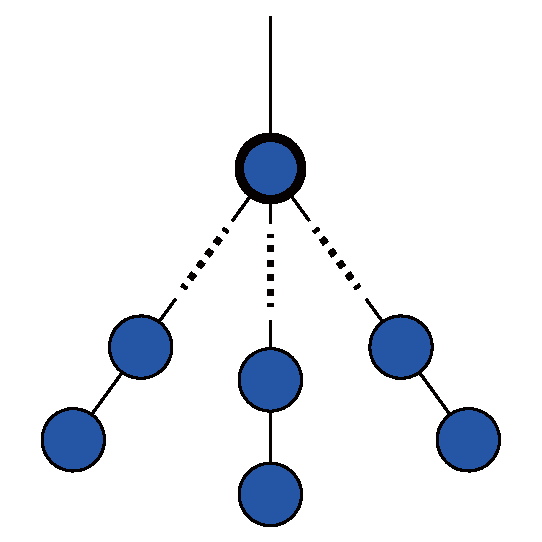
\includegraphics[width = .50\linewidth]{figs/tree}
    \subcaption{ }
  \end{minipage}
  \medskip
  \caption{\textbf{Synchronization of bus bars in a power grid with a tree structure}}
  \label{fig:treepr}
  }
\medskip
\end{figure}
%\begin{figure}[t]
%\centering
%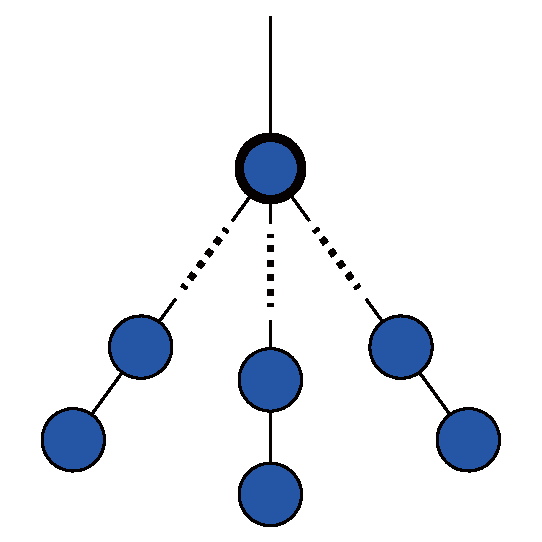
\includegraphics[width = .20\linewidth]{figs/tree}
%\caption{...}
%\label{fig:treepr}
%\medskip
%\end{figure}
There is no limit to the degree of bus bars in a power grid with a tree structure shown in Theorem \ref{thm:tree}.
As such, even if a bus bar with degree of four or higher is included in the power grid, synchronization of all bus bars could be deduced based only on the information from the graph structure.
Similarly, the following fact can be shown.

\begin{theorem}[Synchronization of bus bars in a power grid with a ring structure]
\label{thm:circ}
With simultaneous equations of Equation \ref{eq:PQVgen}, let us consider an electrical power system model where a group of equipment is connected.
When the graph of a power grid has a ring structure, and the total number of bus bars is odd, all bus bars synchronize under a steady power flow distribution.
\end{theorem}

\begin{proof}
Focusing on one bus bar shows the synchronization of the bus bars at both ends of it.
By repeating this process, synchronization of all bus bars is shown when the total number of bus bars is odd.
\end{proof}

%\begin{figure}[t]
%  \centering
%  {
%  \begin{minipage}{0.3\linewidth}
%    \centering
%    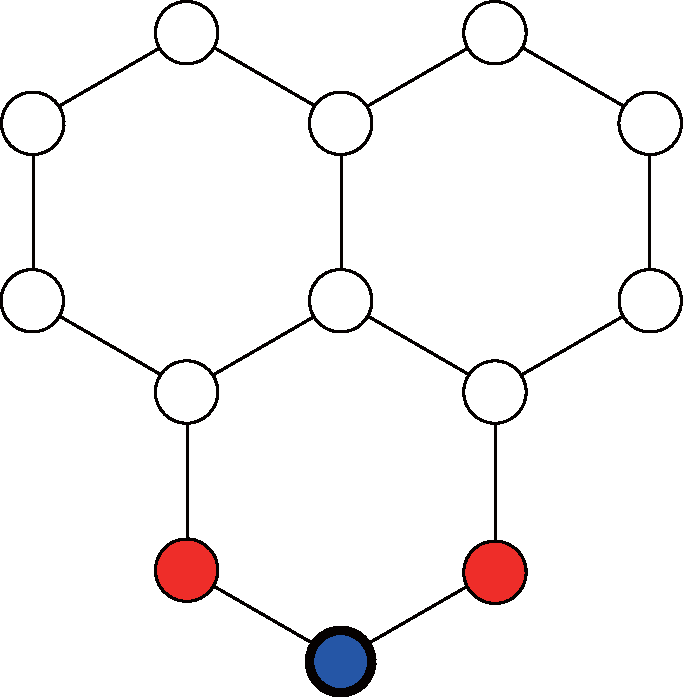
\includegraphics[width = .70\linewidth]{figs/honya}
%    \subcaption{  }
%  \end{minipage}
%  \begin{minipage}{0.3\linewidth}
%    \centering
%    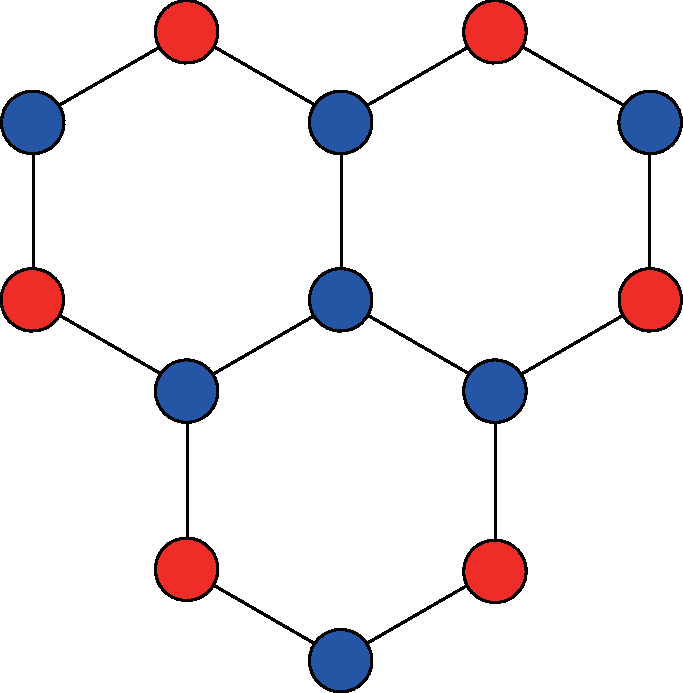
\includegraphics[width = .70\linewidth]{figs/honyb}
%    \subcaption{  }
%  \end{minipage}
%  \begin{minipage}{0.3\linewidth}
%    \centering
%    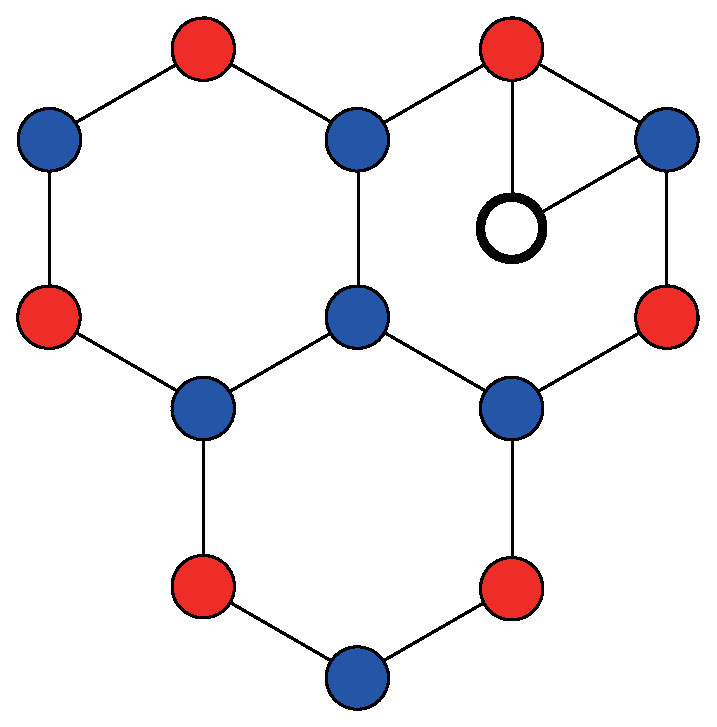
\includegraphics[width = .70\linewidth]{figs/honyc}
%    \subcaption{  }
%  \end{minipage}
%  \medskip
%  \caption{\textbf{ハニカム構造をもつ送電網における母線の同期}}
%  \label{fig:hony}
%  }
%\medskip
%\end{figure}

Theorem \ref{thm:circ} indicates that, in a power grid with a ring structure, if the total number of bus bars is odd, regardless of the admittance of each power grid, all bus bars synchronize.
On the other hand, if the total number of bus bars is even, unless using additional information, such as admittance of transmission lines, synchronization of all bus bars cannot be concluded even for a power grid with a ring structure.
In the Example \ref{ex:symbox} discussed later, even if the total number of bus bars is even, as long as there is some information such as admittance, all bus bars can be synchronized. 

The next example is an application of Lemma \ref{lem:sumc2} to a power grid that includes a bus bar with degree of three.

%次数3の母線を含む送電網にlemma\ref{lem:sumc2}を適用したexampleとしてつぎを示す。

%\begin{example}[ハニカム構造の送電網における母線の同期]\label{ex:deg3}
%Figure \ref{fig:hony}(a)に示されるハニカム構造をもつ送電網に対して,定常潮流状態における母線の同期を考えよう。
%最下部の母線に注目すると,その両隣の母線の同期がわかる。
%これらの同期する母線を赤で示し,最下部の母線と同期するものを青で示す。
%このとき,lemma\ref{lem:sumc2}を各母線に適用していくことによって,同期するすべての母線群をFigure \ref{fig:hony}(b)のように色分けすることができる。
%しかしながら,この場合には,グラフ構造の情報だけで赤の母線群と青の母線群の同期を結論づけることはできない。
%一方で,Figure \ref{fig:hony}(c)のように母線が1つ追加された送電網の場合には,その追加された母線に注目することで,両隣の赤と青の母線の同期が導かれる。
%したがって,Figure \ref{fig:hony}(c)のグラフ構造の場合には,すべての母線の同期が示される。
%\end{example}
%
%example\ref{ex:deg3}において,一部のグラフ構造の差異により同期する母線の対称性が崩れることで,電力系統全体での母線の同期が演繹されている点は興味深い。
%つぎのexampleでは,アドミタンスの値まで考慮した「定量的な送電網の対称性」の観点から母線の同期を考察する。

\begin{figure}[t]
\centering
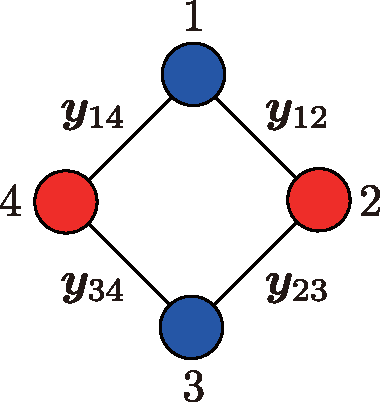
\includegraphics[width = .20\linewidth]{figs/4busbox}
\medskip
\caption{\textbf{円環構造をもつ送電網における4母線の同期}}
\label{fig:4busbox}
\medskip
\end{figure}

\begin{example}[Synchronization of four bus bars in a power grid with a ring structure]\label{ex:symbox}
Let us consider synchronization of bus bars under a steady power flow distribution in a power grid with a ring structure shown in Figure \ref{fig:4busbox}.
Since the number of bus bars is even, synchronization of bus bars cannot be shown using only the information of the graph structure as in Theorem \ref{thm:circ}.
However, as it is shown with red and blue in Figure \ref{fig:4busbox}, synchronization of alternating bus bars is shown by Lemma \ref{lem:sumc2}.
Therefore, for all bus bars to show synchronization, all that is necessary is to show that one of the conditions of Equation \ref{eq:N2sing} is not satisfied for at least one bus bar.

The admittance of the transmission line that connects bus bar $i$ and bus bar $j$ is expressed as $\bm{y}_{ij}$.
At this point, the center condition of Equation \ref{eq:N2sing} for each bus bar can be rewritten as:
\begin{align*}
|\bm{V}_2^{\star}||\bm{y}_{12}|&=|\bm{V}_4^{\star}||\bm{y}_{14}|
,\qquad
|\bm{V}_1^{\star}||\bm{y}_{12}|=|\bm{V}_3^{\star}||\bm{y}_{23}|,
\\
|\bm{V}_2^{\star}||\bm{y}_{23}|&=|\bm{V}_4^{\star}||\bm{y}_{34}|
,\qquad
|\bm{V}_3^{\star}||\bm{y}_{34}|=|\bm{V}_1^{\star}||\bm{y}_{14}|
\end{align*}

If we express this as a matrix:

\begin{align*}
\underbrace{
\mat{
0 & |\bm{y}_{12}| &  0  & -|\bm{y}_{14}|\\
-|\bm{y}_{12}| & 0 & |\bm{y}_{23}| & 0\\
0 & -|\bm{y}_{23}| & 0 & |\bm{y}_{34}|\\
|\bm{y}_{14}| & 0 & -|\bm{y}_{34}| & 0
}}_{S}
\mat{
|\bm{V}_1^{\star}|\\
|\bm{V}_2^{\star}|\\
|\bm{V}_3^{\star}|\\
|\bm{V}_4^{\star}|
}=0
\end{align*}

For conditions necessary for a positive vector that satisfy this Equation $(|\bm{V}_1^{\star}|,\ldots,|\bm{V}_4^{\star}|)$ to exist, $S$ on the left side must be nonsingular.
Because of the sparse structure of the column vector, for $S$ to be non-regular; the following must be true:

\begin{align}\label{eq:ycond}
|\bm{y}_{12}||\bm{y}_{34}| = |\bm{y}_{14}||\bm{y}_{23}|
\end{align}

Therefore, unless the admittance matrix satisfies these conditions, all bus bars synchronize.
If Equation \ref{eq:ycond} is satisfied, the absolute value of the desired voltage phasor can be determined; thus, the condition necessary for $(|\bm{V}_1^{\star}|,\ldots,|\bm{V}_4^{\star}|)$ that satisfies the central condition of Equation \ref{eq:N2sing} to exist is the Equation \ref{eq:ycond}.

Next, the condition of the right side of Equation \ref{eq:N2sing} can be written as below if we focus on bus bar 1 and bus bar 3:
\begin{align*}
|\phi_2 - \phi_4 + \angle \bm{y}_{12} - \angle \bm{y}_{14}|=\pi
,\qquad
|\phi_2 - \phi_4 + \angle \bm{y}_{23} - \angle \bm{y}_{34}|=\pi
\end{align*}

Similarly, if we focus on bus bar 2 and bus bar 4, the following can be obtained:

\begin{align*}
|\phi_1 - \phi_3 + \angle \bm{y}_{12} - \angle \bm{y}_{23}|=\pi
,\qquad
|\phi_1 - \phi_3 + \angle \bm{y}_{14} - \angle \bm{y}_{34}|=\pi
\end{align*}

Generally, when capacitance to ground is sufficiently small, the real part of admittance, the conductance component, was non-negative, while the imaginary part, the susceptance component, was negative.
In other words:

\[
\angle \bm{y}_{ij} \in \left[-\frac{\pi}{2},0 \right]
\]

If we focus on this, the condition necessary for $(\phi_1,\ldots,\phi_4)$ that satisfies the above conditions to exist is derived as:

\begin{align}\label{eq:ycona}
\angle \bm{y}_{12} - \angle \bm{y}_{14}=
\angle \bm{y}_{23} - \angle \bm{y}_{34}
\end{align}
Therefore, as long as the admittance matrix does not satisfy this condition, all bus bars synchronize.

The above discussion shows that the conditions necessary for at least one set of bus bars that do not synchronize under a steady power flow distribution to exist are Equation \ref{eq:ycond} and Equation \ref{eq:ycona}.
These two conditions indicate that only when the power grid of Figure \ref{fig:4busbox} has specific symmetry related to the admittance value, a condition arises where only alternating bus bars synchronize.
\end{example}

The Example \ref{ex:symbox} shows that the condition of Equation \ref{eq:N2sing} presents specific symmetry related to the admittance of the power grid.
In a practical application, all bus bars synchronizing under a steady power flow distribution for a sparse grid where each bus has a low degree is a universal fact as long as there is no specific symmetry in the graph structure.
Actually, as far as the author is aware, synchronization of all bus bars under a steady power flow distribution has been numerically confirmed for all parameters of the electric power system model that are set to realistic values. 


\section{Method to implement the power flow calculation}\label{sec:powfcal}
\red{Translated with DeepL}
We consider building a numerical simulation environment for power system analysis and control.
In order to correctly implement numerical simulation of a large and complex power system model, object-oriented thinking and programming techniques that describe the model as a group of modules divided by function are useful.
In this section, we describe an implementation method for tidal current calculation based on this way of thinking.


\subsection{How to solve algebraic equations}
For the power flow calculation, simultaneous equations of Equation \ref{eq:ohmY2} must be solved.
In this Section, we will first use a simple problem to show a method to search the solution of algebraic equations with \matlab.

\begin{example}[Searching for a solution for algebraic equations]\label{ex:algenraic_equation_ex1}
Let us consider a set of $(x, y)$ that satisfies algebraic equations through numerical calculation: 
\begin{subequations}\label{eq:algebraic_equation_ex1}
\begin{align}
x^2 - y = 0\\
x^2 + y^2 - 2 = 0
\end{align}
\end{subequations}
Please note that there are two solutions: $(-1, 1)$ and $(1, 1)$. \verb|fsolve| of \verb|optimization toolbox| is a convenient command that solves algebraic equations in \matlab.
To use this command, function $f(x,y)$ must be implemented, where algebraic equations of Equation (\ref{eq:algebraic_equation_ex1}) are expressed as follows:
\[
f(x,y)=0
\]
When this function is implemented with a file name of \verb|func_ex1.m|, it is called program \nobreak\ref{program:ex1}.

\smallskip
\begin{PROGRAMA}[count,title={func\_ex1.m}]\label{program:ex1}
\begin{verbatim}
function out = func_ex1(x_in)

x = x_in(1);
y = x_in(2);

out = zeros(2, 1);
out(1) = x^2 - y;
out(2) = x^2 + y^2 - 2;

end
\end{verbatim}
\end{PROGRAMA}

Next, if a program is written to execute \verb|fsolve| using this function and search for a solution for algebraic equations, it becomes program \nobreak\ref{program:ex1_main}:
\smallskip
\begin{PROGRAMA}[count,title={main\_ex1.m}]\label{program:ex1_main}
\begin{verbatim}
options = optimoptions('fsolve', 'Display', 'iter');
x0 = [0.1; 0.5];
x_sol = fsolve(@func_ex1, x0, options)
\end{verbatim}
\end{PROGRAMA}

Here \verb|options| in the first row sets the optimum option that converges $f(x,y)$ to 0.
With this example, the optimization process is shown. \verb|x0 = [0.1; 0.5];| in the second row shows the initial value at the time of optimization with convergence calculation.
When we execute this program, the following result is obtained:

\smallskip
\begin{execution}
\begin{verbatim}
  Iteration  Func-count     f(x)     (省略)
      0          3          3.2677
      1          6        0.282554
(省略)
      4         15     3.60447e-14

  方程式が解かれました。
(省略)
  x_sol =
      1.0000
      1.0000
\end{verbatim}
\end{execution}

Based on this result, with repetitions, the value of $f(x)$ becomes small, and ultimately, a solution is found where $f(x)$ becomes almost 0.
The solution sought here is $(1, 1)$. This value is an actual solution to algebraic equations, but in a numerical solution that uses \verb|fsolve|, not all solutions are obtained, as only one solution is obtained.

Next, let us look at a situation where another solution is obtained.
The next result is obtained when the second row of the program \nobreak\ref{program:ex1_main} is changed to \verb|x0 = [-0.1; 0.5];|.

\smallskip
\begin{execution}
\begin{verbatim}
 Iteration  Func-count     f(x)   
     0          3          3.2677
     1          6        0.282554
(省略)
     4         15     3.60447e-14

方程式が解かれました。
(省略)
x_sol =

   -1.0000
    1.0000
\end{verbatim}
\end{execution}

We can see that the solution $(-1, 1)$ is obtained.
As such, with the numerical solution of non-linear algebraic equations, the solution varies based on the initial value.
As a reference, let us look at the result of executing the program \nobreak\ref{program:ex1_main} with the initial value in the second row set as \verb|x0 = [-0.1; -0.1];|:

\smallskip
\begin{execution}
    \begin{verbatim}
  Iteration  Func-count     f(x)     (省略)
     0          3          2.8125
     1          6         1.89068
(省略)
    29         62            1.75

解が見つかりませんでした。
(省略)
x_sol =

    0.0000
   -1.2247
\end{verbatim}
\end{execution}

As you can see with this Example, based on the initial value, even equations with solutions might not yield correct solutions.
For practice, it is important to provide initial values that are close to the desired solution.
\end{example}

\subsection{Simple implementation of the power flow calculation}

Next, let us introduce a simple method to implement a program that performs power flow calculations.

\begin{example}[Implementation method of power flow calculations]\label{ex:simplepowerflow}
Let us think about performing power flow calculations for the power system in Figure \ref{dummy}.
Power flow calculation is a type of calculation to solve algebraic equations. Thus, as in the Example \nobreak\ref{ex:algenraic_equation_ex1}, $f(x)$ of $f(x)=0$ must be implemented.

Let us think about obtaining the steady power flow distribution that is consistent with the datasheet of \ref{table:pflow2}(a) when setting the admittance of two transmission lines to the value of Equation \ref{eq:rightlossless}. 
%\[
%\bigl(
%|\bm{I}_1^{\star}|,\angle \bm{I}_1^{\star},
%|\bm{V}_1^{\star}|,\angle \bm{V}_1^{\star},
%\ldots,
%|\bm{I}_3^{\star}|,\angle \bm{I}_3^{\star},
%|\bm{V}_3^{\star}|,\angle \bm{V}_3^{\star}
%\bigr)
%\]
\[
\bigl(
|\bm{I}_1^{\star}|,\angle \bm{I}_1^{\star},
|\bm{V}_1^{\star}|,\angle \bm{V}_1^{\star},
|\bm{I}_2^{\star}|,\angle \bm{I}_2^{\star},
|\bm{V}_2^{\star}|,\angle \bm{V}_2^{\star},
|\bm{I}_3^{\star}|,\angle \bm{I}_3^{\star},
|\bm{V}_3^{\star}|,\angle \bm{V}_3^{\star}
\bigr)
\]
%    \centering
%     \caption{潮流計算のためのデータシート}\label{tab:datasheet_ex2}
%      \begin{tabular}{cccccc}
%        $i$ & 種類 & $|\bm V_i|$ & $\angle \bm V_i$ & $P_i$ & $Q_i$\\\hline\hline
%        1 & スラック & 2 & 0 & - & -\\
%        2 & 負荷 & - & - & $-3$ & 0 \\
%        3 & 発電機 & 2 & - & 0.5  & - \\
%        \hline
%      \end{tabular}
%\end{table}
When the admittance matrix $\bm Y$ is provided, current is determined uniquely dependent on voltage; thus, power flow calculation becomes a practical step by which to determine a set of voltages.
As such, variables $x$ in algebraic equations just need to be the voltage phasor of bus bars under a steady state.
Here, we express the real and imaginary parts of the voltage phasor of all bus bars in a line as $x$.

\footnote{It is the same when expressing the absolute value and argument of the voltage phasor as $x$}。
As discussed above, the voltage phasor and current phasor of each bus bar can be expressed as a function of $x$.
Similarly, the active power and reactive power of each bus bar also become a function of $x$.
If these are expressed as $\hat{\bm V}_i(x)$, $\hat{\bm I}_i(x)$, $\hat{P}_i(x)$, and $\hat{Q}_i(x)$, algebraic equations to be solved are:
\begin{align*}
    |\bm V_1^{\star}|-|\hat{\bm V}_1(x)| &= 0\\
    \angle \bm V_1^{\star} - \angle \hat{\bm V}_1(x) &= 0\\
    P_2^{\star} -\hat P_2(x) &= 0\\
    Q_2^{\star} -\hat Q_2(x) &= 0\\
    P_3^{\star} -\hat P_3(x) &= 0\\
    |\bm V_3^{\star}|-|\hat{\bm V}_3(x)| &= 0
 \end{align*}
 If we implement the functions on the left side, it becomes a program \nobreak\ref{program:ex2}.

 Though this function has five output arguments, with \texttt{fsolve}, only the first output argument is used.
 The remaining arguments were added to confirm the result.


\smallskip
\begin{PROGRAMA}[count, title={func\_ex2.m}]\label{program:ex2}
\begin{verbatim}
function [out, Vhat, Ihat, Phat, Qhat] = func_ex2(x)
% x: [Real(V1), Imag(V1),
%     Real(V2), Imag(V2),
%     Real(V3), Imag(V3)]';

y12 = 1.3652 - 11.6040j;
y23 = -10.5107j;
Y = [y12, -y12, 0;
    -y12, y12+y23, -y23;
    0, -y23, y23];

V1abs = 2;
V1angle = 0;

P2 = -3;
Q2 = 0;

P3 = 0.5;
V3abs = 2;

V1hat = x(1) + 1j*x(2);
V2hat = x(3) + 1j*x(4);
V3hat = x(5) + 1j*x(6);

Vhat = [V1hat; V2hat; V3hat];

Ihat = Y*Vhat;
PQhat = Vhat.*conj(Ihat);
Phat = real(PQhat);
Qhat = imag(PQhat);

out = [V1abs-abs(V1hat); V1angle-angle(V1hat);
    P2-Phat(2); Q2-Qhat(2);
    P3-Phat(3); V3abs-abs(V3hat)];
end
\end{verbatim}
\end{PROGRAMA}

As discussed in the Example \nobreak\ref{ex:algenraic_equation_ex1}, if searching the solution of algebraic equations with convergence calculation, setting of the initial value is important.
An initial value often used by the power flow calculation is \textbf{flat start}. With flat start, for all bus bars, the initial value of $x$ is set as:
\[
|\hat{\bm V}_i(x)|=1
,\qquad
\angle \bm V_i(x) = 0
\]
This corresponds to setting the real and imaginary parts of $\bm V_i$ of 1 and 0, respectively.
The program is as follows:

\smallskip
\begin{PROGRAMA}[count,title={main\_ex2.m}]\label{program:ex2_main}
\begin{verbatim}
x0 = [1; 0; 1; 0; 1; 0];
options = optimoptions('fsolve', 'Display', 'iter');
x_sol = fsolve(@func_ex2, x0, options);

[~, V, I, P, Q] = func_ex2(x_sol);
Vabs = abs(V);
Vangle = angle(V);
display('Vabs:'), display(Vabs')
display('Vangle:'), display(Vangle')
display('P:'), display(P')
display('Q:'), display(Q')
\end{verbatim}
\end{PROGRAMA}

The initial value is set in the first row. The result of executing the program \nobreak\ref{program:ex2_main} is shown.
This result is consistent with the values shown in \ref{table:pflow2}(b).

\smallskip
\begin{execution}
\begin{verbatim}
 Iteration  Func-count     f(x)     (略)
     0          7           11.25 
     1         14         3.28327 
(省略)
     5         42     4.19428e-28

方程式が解かれました。
(省略)
Vabs:
    2.0000    1.9918    2.0000

Vangle:
    0.0000   -0.0538   -0.0419

P:
    2.5158   -3.0000    0.5000

Q:
   -0.0347    0.0000    0.1759
\end{verbatim}
\end{execution}

\end{example}

% \begin{COLUMN}
% example\nobreak\ref{ex:algenraic_equation_ex2}
% % のプログラムでは,各種のパラメータは\verb{func_ex2.m}の中で
% % 定義されている。様々な条件での潮流計算を行うことを考えて,
% % \verb{main_ex2.m}のファイルにパラメータを記述したくなることがある。
% % グローバル変数はあかん。
% \end{COLUMN}
\subsection{Implementation method of the power flow calculation that considers increased scale}
In the previous section, we discussed the implementation method of the power flow calculation.
With this implementation, each time the admittance matrix is changed, the function related to the program \ref{program:ex2} must be rewritten.
Furthermore, when the number or type of bus bars are changed, the entire program must be rewritten.
In this Section, we consider dividing the program into modules so that power flow calculations can be performed for a large-scale electrical power system and the program can be shared and implemented by multiple people.
In this manner, the program becomes structured and clear.
First, let us think about separating the implementation of the admittance matrix of the program \nobreak\ref{program:ex2}.

First, let us think about separating the implementation of the admittance matrix of the program \nobreak\ref{program:ex2}.

\begin{example}[Separation of the implementation of the admittance matrix]
In the program \nobreak\ref{program:ex2}, let us separate the part that specifies the admittance matrix.
To do this, the function of variables \verb|Y| is used as the input argument.
For example, the following correction is possible.

\smallskip
\begin{PROGRAMA}[count, title={func\_ex3.m}]\label{program:ex3}
\begin{verbatim}
function [out, Vhat, Ihat, Phat, Qhat] = func_ex3(x, Y)
(Same as lines 12 through 34 of program 3-3)
end
\end{verbatim}
\end{PROGRAMA}

However, the specification of \verb|fsolve| demands a function that uses the optimizing parameter as the only argument; thus, the program \ref{program:ex3} cannot be used directly.
This problem can be solved by using a technology called \textbf{currying} for the function.
Specifically, it is corrected as follows:

\smallskip
\begin{PROGRAMA}[count,title={main\_ex3.m}]\label{program:ex3_main}
\begin{verbatim}
x0 = [1; 0; 1; 0; 1; 0];
options = optimoptions('fsolve', 'Display', 'iter');

y12 = 1.3652 - 11.6040j;
y23 = -10.5107j;
Y = [y12, -y12, 0;
    -y12, y12+y23, -y23;
    0, -y23, y23];

func_curried = @(x) func_ex3(x, Y);

x_sol = fsolve(func_curried, x0, options);
[~, V, I, P, Q] = func_curried(x_sol);
(プログラム3-4の6行目以下と同じ)
\end{verbatim}
\end{PROGRAMA}

\red{Translated with www.DeepL.com/Translator (free version)}
The "\verb|@(x) expression of x|" used creates "a function that returns an expression of \verb|x| for the argument \verb|x|".
In this way, a function that is generated without writing the function name is called \textbf{anonymous function}.
In this case, the variable \verb|Y|, which is not included in the argument of the anonymous function, is always a constant that exists in the workspace.
This allows us to generate a new function that retains only the first argument,\verb|x|, of the two input arguments,\verb|x| and \verb|Y|, of the function \verb|func_ex3(x, Y)|.


\red{Translated with www.DeepL.com/Translator (free version)}
Thus, culling is the creation of a new function in which the variables given to some of the multiple arguments are fixed and only the remaining variables are used as arguments.
Using this technique, a function with an arbitrary number of arguments can be used as a function with the required number of arguments.
This allows separation of functions without the use of global variables.

\end{example}

\red{Translated with DeepL}
Next, consider the part of the program\nobreak\ref{program:ex2} that calculates the constraint conditions at each bus bar.
In the program\nobreak\ref{program:ex2}, the constraint conditions for each bus bar are written down directly, so the program needs to be rewritten each time the number of bus bars is changed.
In addition, the case classification by the type of bus bar is implicitly included, which means that the case classification process needs to be modified when the number of bus bars is increased.

In order to write a program with good visibility without using case separation, it is recommended to use the object-oriented concept of \textbf{polymorphism}.
In the following examples, the idea of polymorphism will be explained through implementation examples.

\begin{example}[Separation of bus bar implementation]
In the power flow calculation, different constraints are set based on different types of bus bars.
At this time, the bus bar of each type has a commonality of “having constraints”.
If we implement this common property as a method with a common name, we can create a program that is easy to handle.
Specifically, the class of bus bars is defined as shown in Program \ref{program:bus_slack} to Program \ref{program:ex4}.
If we use the instance of these classes, the power flow calculation can be executed as below.

\smallskip
\begin{PROGRAMA}[count,title={bus\_slack.m}]\label{program:bus_slack}
\begin{verbatim}
classdef bus_slack
  
  properties
    Vabs
    Vangle
  end
  
  methods
    function obj = bus_slack(Vabs, Vangle)
      obj.Vabs = Vabs;
      obj.Vangle = Vangle;
    end
    
    function out = get_constraint(obj, Vr, Vi, P, Q)
      Vabs = norm([Vr; Vi]);
      Vangle = atan2(Vi, Vr);
      out = [Vabs-obj.Vabs; Vangle-obj.Vangle];
    end
  end
end
\end{verbatim}
\end{PROGRAMA}

\smallskip
\begin{PROGRAMA}[count,title={bus\_genertor.m}]\label{program:bus_PV}
\begin{verbatim}
classdef bus_generator
  
  properties
    P
    Vabs
  end
  
  methods
    function obj = bus_generator(P, Vabs)
      obj.P = P;
      obj.Vabs = Vabs;
    end
    
    function out = get_constraint(obj, Vr, Vi, P, Q)
      Vabs = norm([Vr; Vi]);
      out = [obj.P-P; Vabs-obj.Vabs];
    end
  end
end
\end{verbatim}
\end{PROGRAMA}

\smallskip
\begin{PROGRAMA}[count,title={bus\_load.m}]\label{program:bus_PQ}
\begin{verbatim}
classdef bus_load
  
  properties
    P
    Q
  end
  
  methods
    function obj = bus_load(P, Q)
      obj.P = P;
      obj.Q = Q;
    end
    
    function out = get_constraint(obj, Vr, Vi, P, Q)
      out = [P-obj.P; Q-obj.Q];
    end
  end
end
\end{verbatim}
\end{PROGRAMA}

\smallskip

\red{Translated with DeepL}
All of the classes defined here, \verb|bus_slack|, \verb|bus_generator|, and \verb|bus_load|, have a method named \verb|get_constraint| with common inputs and outputs.
In this case, programs using these classes can calculate constraints appropriately by calling \verb|get_constraint| without being aware of which type of bus bar they are.
If we rewrite the Program \nobreak\ref{program:ex2} using this concept, we obtain the following.


\smallskip
\begin{PROGRAMA}[count, title={func\_power\_flow.m}]\label{program:ex4}%
\begin{verbatim}
function [out, V, I, P, Q] = func_power_flow(x, Y, a_bus)

V = x(1:2:end) + 1j*x(2:2:end);
I = Y*V;
PQhat = V.*conj(I);
P = real(PQhat);
Q = imag(PQhat);

out_cell = cell(numel(a_bus), 1);

for i = 1:numel(a_bus)
  bus = a_bus{i};
  out_cell{i} = bus.get_constraint(...
    real(V(i)), imag(V(i)), P(i), Q(i));
end
out = vertcat(out_cell{:});

end
\end{verbatim}
\end{PROGRAMA}

\red{Translated with DeepL}
The program \nobreak\ref{program:ex4} assumes that the cell array, which is the set of mother lines, is input as \verb|a_bus|.
An example of how to use this function is shown in the program \nobreak\ref{program:ex4_main}.

\smallskip
\begin{PROGRAMA}[count,title={main\_ex4.m}]\label{program:ex4_main}
\begin{verbatim}
(Same as lines 1-8 in program 3-6)

a_bus = cell(3, 1);
a_bus{1} = bus_slack(2, 0);
a_bus{2} = bus_load(-3, 0);
a_bus{3} = bus_generator(0.5, 2);

func_curried = @(x) func_power_flow(x, Y, a_bus);

x_sol = fsolve(func_curried, x0, options);

(Same as Program 3-4, line 6 and following)
\end{verbatim}
\end{PROGRAMA}

\red{Translated with DeepL until end of chapter}
In the program \nobreak\ref{program:ex4_main}, the slack bus bar, load bus bar, and generator bus bar are defined respectively and assigned to the cell array \verb|a_bus|.
At this time, in the program\nobreak\ref{program:ex4}, \verb|get_constraint| is executed for each bus bar assigned to \verb|a_bus|.
Since \verb|get_constraint| is implemented for each bus line type, the appropriate processing is performed without having to describe the case.
Such different processing for similar program calls is called {polymorphism} or {polymorphism}, and is one of the important concepts in object-oriented programming.


\begin{comment}
In the implementation of the program \nobreak\ref{program:ex4_main}, the constraint is computed by calling a method named \verb|get_constraint| method, which has a common name without being aware of the type of bus bar.
\red{(called in programs 1-10, not 3-11?). Also, is the backslash before the underscore unnecessary?}.
The description is simplified.
This property of being able to use the same method name regardless of the type of instance is called \textbf{polymorphism} or \textbf{polymorphism}, and is one of the important concepts in object-oriented programming.
Using polymorphism not only simplifies not only simplifies the description, but also
\end{comment}

An implementation using polymorphism such as Program \nobreak\ref{program:ex4} has the advantage that it is easy to deal with changes in the number or configuration of bus bars.
That is, the Program \nobreak\ref{program:ex4_main} can be used without modification simply by changing the number and definition of bus bars in lines 3 to 6 of the Program \nobreak\ref{program:ex4_main}.

Furthermore, it is easy to add new types of bus bars.
The program \nobreak\ref{program:ex4} assumes only that there exists a method named \verb|get_constraint| with appropriate inputs and outputs for the bus bar.
In other words, if it has a \verb|get_constraint|, it is defined to be a bus bar.
This is a concept called duck typing, derived from "if it walks like a duck and quacks like a duck, then it is a duck".
This allows the module designer to define a new class of bus bar and implement only \verb|get_constraint| without paying attention to the internal processing of the program \nobreak\ref{program:ex4}.
In other words, this clarifies the scope of the implementation to be done by the module designer.
\end{example}

The above has allowed us to prospectively implement a program for calculating the tidal currents given an admittance matrix.
Furthermore, let us implement the computation of the admittance matrix by dividing it into a group of modules.

\begin{example}[Object-oriented computation of admittance matrices]
An admittance matrix is generally defined by several transmission lines.
Therefore, we consider creating a class that represents a transmission line and using a set of instances of the class.
Since a transmission line connects two bus bars, the numbers of those bus bars need to be specified.
In addition, in general, regardless of the type of transmission line model
\begin{align}
\mat{
\bm I_\mathrm{from}\\\bm I_\mathrm{to}
} =
\bm Y_\mathrm{branch}
\mat{
\bm V_\mathrm{from}\\\bm V_\mathrm{to}
}
\end{align}

The admittance matrix $\bm Y_\mathrm{branch}$ is determined satisfying where $\bm V_\mathrm{from}$ and $\bm V_\mathrm{to}$ are the voltages at the bus bars at both ends of the transmission line and $\bm I_\mathrm{from}$ and $\bm I_\mathrm{to}$ are the currents entering the transmission line from the bus bars at both ends.
For example, for the simple transmission line treated in the example\ref{ex:derY}

\[
\bm Y_\mathrm{branch} = \begin{bmatrix}
\bm y & -\bm y\\
-\bm y & \bm y
\end{bmatrix}
\]

In summary, if the information on the bus bar at both ends and the admittance matrix $Y_\mathrm{branch}$ are returned, it is safe to define it as a transmission line.
An example implementation of a transmission line based on this concept is shown below.

\smallskip
\begin{PROGRAMA}[count,title={branch.m}]\label{program:branch}
\begin{verbatim}
classdef branch
  
  properties
    y
    from
    to
  end
  
  methods
    function obj = branch(from, to, y)
      obj.from = from;
      obj.to = to;
      obj.y = y;
    end
    
    function Y = get_admittance_matrix(obj)
      y = obj.y;
      Y = [y, -y;
        -y,  y];
    end
  end
end
\end{verbatim}\end{PROGRAMA}

The function to compute the admittance matrix using this transmission line class is implemented as follows
%\footnote{ここでは,母線のシャント抵抗は簡単のために無視する。}。
\smallskip
\begin{PROGRAMA}[count,title={get\_admittance\_matrix.m}]\label{program:admittance}
\begin{verbatim}
function Y = get_admittance_matrix(n_bus, a_branch)

Y = zeros(n_bus, n_bus);

for i = 1:numel(a_branch)
  br = a_branch{i};
  Y_branch = br.get_admittance_matrix();
  Y([br.from, br.to], [br.from, br.to]) =...
    Y([br.from, br.to], [br.from, br.to]) + Y_branch;
end

end
\end{verbatim}
\end{PROGRAMA}

The input argument \verb|n_bus| is the number of bus lines.
Also, \verb|a_branch| is a cell array containing the transmission lines.
This program can be used as follows

\smallskip
\begin{PROGRAMA}[count,title={main\_admittance\_matrix.m}]\label{program:main_admittance}
\begin{verbatim}
a_branch = cell(2, 1);
a_branch{1} = branch(1, 2, 1.3652-11.6040j);
a_branch{2} = branch(2, 3, -10.5107j);

Y = get_admittance_matrix(3, a_branch)
\end{verbatim}
\end{PROGRAMA}


In the program\nobreak\ref{program:admittance}, we only assume that the transmission line has the data \verb|from| and \verb|to| and that it has the method \verb|get_admittance_matrix| and the method \verb|get_admittance_matrix|.
Therefore, when considering other transmission line models such as $\pi$-type models When considering other transmission line models, such as $\pi$-type models, the variables \verb|to| and \verb|from| and the method \verb|get_admittance_matrix| are also assumed to be used.
The program program \nobreak\ref{program:admittance} can be used without any modification by simply implementing a class with variables named \verb|to|, \verb|from| and a method named \verb|get_admittance_matrix|.
\end{example}

From the above, the program to calculate tidal currents can be summarized as follows.

\begin{example}[Tidal current calculation implementation results]
\red{Translated with DeepL}
The program implemented in the above example is summarized and organized as a function that performs a tidal flow calculation Program\nobreak\ref{program:calc_flow}.

\smallskip
\begin{PROGRAMA}[count,title={calculate\_power\_flow.m}]\label{program:calc_flow}
\begin{verbatim}
function [V, I, P, Q] = calculate_power_flow(a_bus, a_branch)

n_bus = numel(a_bus);
Y = get_admittance_matrix(n_bus, a_branch);

func_curried = @(x) func_power_flow(x, Y, a_bus);

x0 = kron(ones(n_bus, 1), [1; 0]);
options = optimoptions('fsolve', 'Display', 'iter');
x_sol = fsolve(func_curried, x0, options);

[~, V, I, P, Q] = func_curried(x_sol);

end
\end{verbatim}
\end{PROGRAMA}

\red{Translated with DeepL}
This program receives a set of bus lines and a set of transmission lines and performs a tidal current calculation It can be used as Program \nobreak\ref{program:main_calc_flow}.

\smallskip
\begin{PROGRAMA}[count,title={main\_power\_flow.m}]\label{program:main_calc_flow}
\begin{verbatim}
a_bus = cell(3, 1);
a_bus{1} = bus_slack(2, 0);
a_bus{2} = bus_load(-3, 0);
a_bus{3} = bus_generator(0.5, 2);

a_branch = cell(2, 1);
a_branch{1} = branch(1, 2, 1.3652-11.6040j);
a_branch{2} = branch(2, 3, -10.5107j);

[V, I, P, Q] = calculate_power_flow(a_bus, a_branch);

display('Vabs:'), display(abs(V)')
display('Vangle:'), display(angle(V)')
display('P:'), display(P')
display('Q:'), display(Q')
\end{verbatim}
\end{PROGRAMA}

\red{Translated with DeepL}
If it is necessary to perform tidal flow calculations for different power grids, only the definitions of bus bar and transmission line in lines 1 to 8 of the Program \nobreak\ref{program:main_calc_flow} can be changed, and the other programs can be used without any modification.
When a new type of bus bar or transmission line is needed, a new class that implements the data and methods with the defined names can be implemented.
These features make the program more readable and extensible than a simple implementation such as \ref{ex:simplepowerflow}.
\end{example}

\section{How to implement time response calculations for power system models}\label{sec:timerescal}

\red{Translated with DeepL}
This section describes how to numerically calculate the time response of a power system model using \matlab.
The computation of the time response of a power system model requires solving a system of differential equations that expresses the dynamic characteristics of the equipment and a system of differential algebraic equations that The time response of the power system model requires solving a system of differential algebraic equations, which is a system of differential equations representing the dynamic characteristics of the equipment and a system of algebraic equations for the power flow.
First, let's take a simple system of differential-algebraic equations as an example and see how to solve it.

\begin{figure}[t]
  \centering
  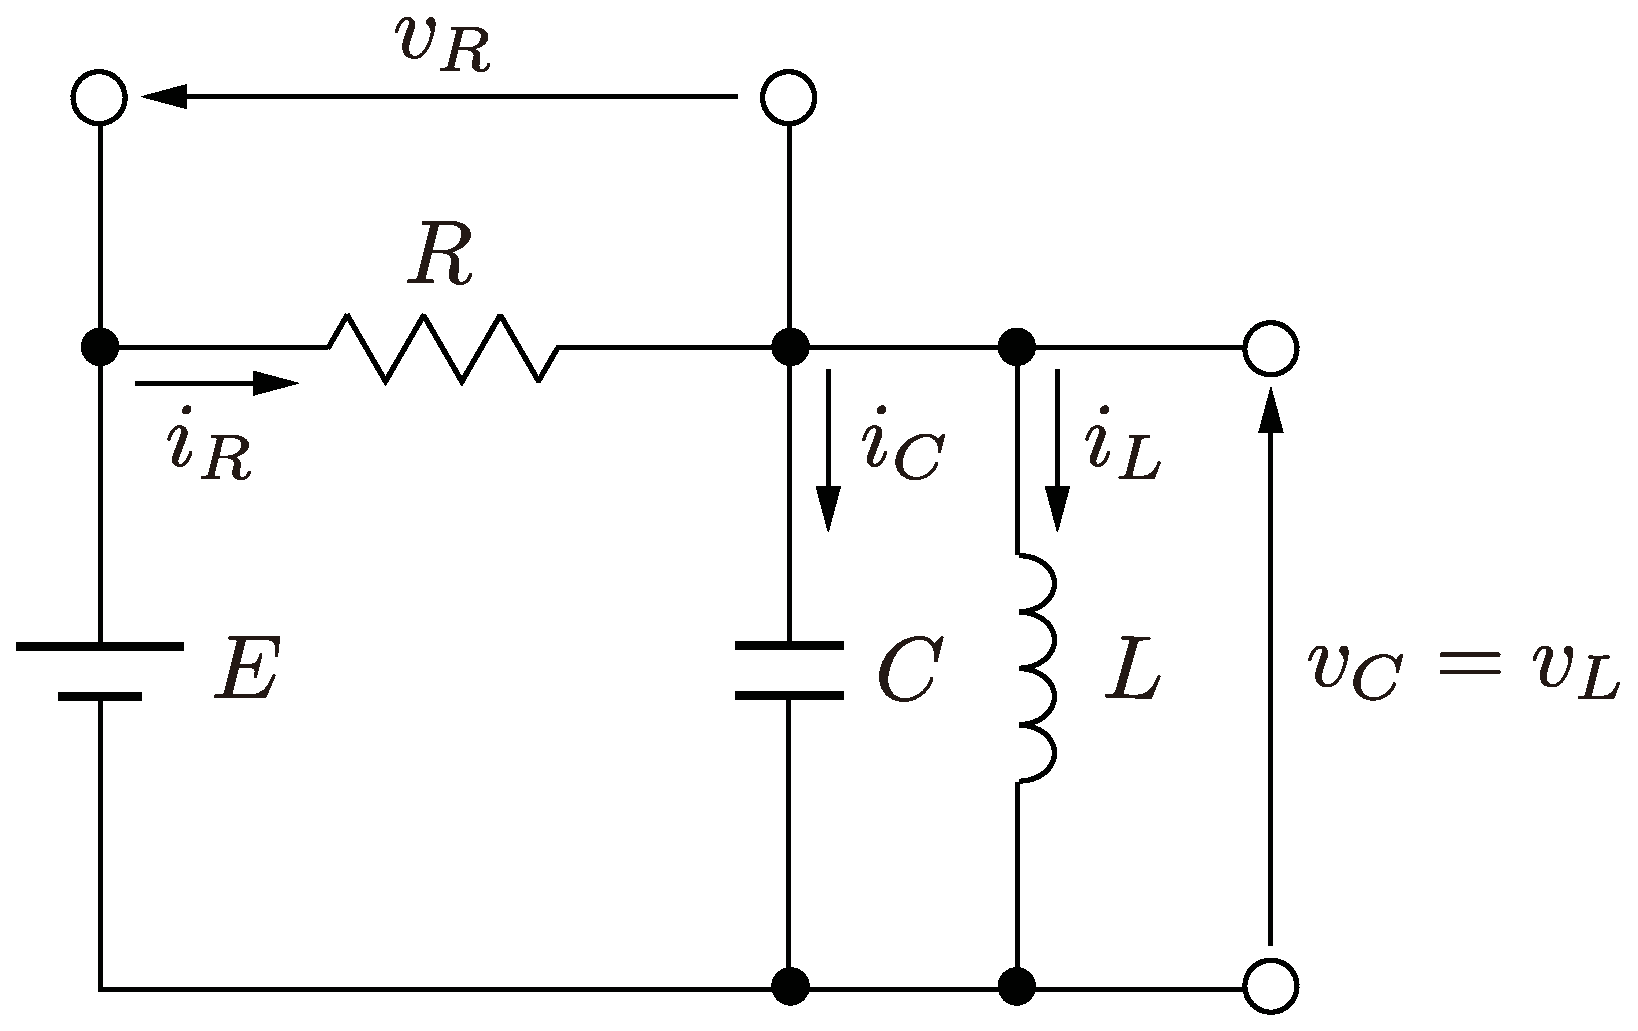
\includegraphics[width = .5\linewidth]{figs/circkawaguchi}
  \medskip
  \caption{\textbf{Differential Algebraic Equations Example: LC Parallel Circuit}}
  \label{fig:RLC}
  \medskip
\end{figure}


\begin{example}[Numerical solution of simple systems of differential-algebraic equations]\label{ex:dae_ex1}
\red{Translated with DeepL}
Numerical simulation is performed for the simple electric circuit shown in Figure \ref{fig:RLC}, where $R$, $L$, $C$, and $E$ are all 1.
The dynamic elements of this circuit are the coil $L$ and the capacitor $C$, whose differential equations are given by:
\begin{subequations}\label{eq:ex_de}
  \begin{align}
    L\dot i_L & = v_L \\
    C\dot v_C & = i_C
  \end{align}
\end{subequations}
However, the initial values are $i_L(0)=0$ and $v_C(0)=0$.
Also, from Ohm's law and Kirchhoff's law, we get the following algebraic equations.
\begin{subequations}\label{eq:ex_ae}
  \begin{align}
    v_R & =R i_R      \\
    i_R & = i_L + i_C \\
    v_L & = v_C       \\
    E   & = v_C + v_R
  \end{align}
\end{subequations}

Using the algebraic equations in equation (\ref{eq:ex_ae}) and eliminating redundant variables such as $v_R$ and $i_R$, we obtain an equivalent system of ordinary differential equations can be obtained.
This operation corresponds to Kron reduction, and the resulting system of ordinary differential equations is
\begin{subequations}\label{eq:ex1_ode}
  \begin{align}
    \dot{i}_L & = \frac{1}{L}v_C                     \\
    \dot{v}_C & = \frac{1}{RC}(E-v_C)-\frac{1}{C}i_L
  \end{align}
\end{subequations}

First, let's write a program to solve this ordinary differential equation system.
The solver of \matlab for the ODE system is generally \verb|ode45|.
In \verb|ode45|, the solution of the ordinary differential equation system can be obtained by implementing the function $f(t,x)$ of the ordinary differential equation $\dot{x} = f(t,x) $.
Implementing the right-hand side of an expression (\ref{eq: ex1_ode}) results in the Program \ref{program: ex1_ode}.

\smallskip
\begin{PROGRAMA}[count,title={func\_RLC\_ode.m}]\label{program:ex1_ode}
  \begin{verbatim}
function dx = func_RLC_ode(x, R, C, L, E)

iL = x(1);
vC = x(2);

diL = vC/L;
dvC = (E-vC)/R/C - iL/C;

dx = [diL; dvC];

end
\end{verbatim}
\end{PROGRAMA}

As a result, when \verb|ode45| is executed and the ordinary differential equation system is solved, the program \nobreak\ref{program: main_ode1} becomes:

\smallskip
\begin{PROGRAMA}[count,title={main\_RLC\_ode.m}]\label{program:main_ode1}
\begin{verbatim}
R = 1;
L = 1;
C = 1;
E = 1;

func = @(t, x) func_RLC_ode(x, R, C, L, E);
x0 = [0; 0];
tspan = [0 30];

[t, x] = ode45(func, tspan, x0);

plot(t, x)
\end{verbatim}
\end{PROGRAMA}

The output variable \verb|x| in the program \nobreak\ref{program: main_ode1} is a matrix in which the time series of $i_L$ and $v_C$ are arranged vertically.
Therefore, note that the time series of other variables such as $i_C$ and $i_R$ need to be additionally calculated using the algebraic equation of the equation (\ref{eq: ex_ae}).

Next, consider directly finding the solution of the system of differential algebra equations without going through Kron reduction.
In this case, since the physical algebraic equation can be written down as it is, there is an advantage that the description is easy even if the system becomes complicated.
One of the commands that can solve the system of differential algebra with \matlab is \verb|ode15s|.
The target is a system of differential algebraic equations described in the following format.
\begin{align}\label{eq:numDAE}
  M\dot{x} = f(t, x)
\end{align}
Applying the expression (\ref{eq: ex_de}) and the expression (\ref{eq: ex_ae}):
\[
\underbrace{
\mat{
    0 & L & 0 & 0 & 0 & 0 \\
    0 & 0 & 0 & 0 & 0 & C \\
    0 & 0 & 0 & 0 & 0 & 0 \\
    0 & 0 & 0 & 0 & 0 & 0 \\
    0 & 0 & 0 & 0 & 0 & 0 \\
    0 & 0 & 0 & 0 & 0 & 0 \\
}
}_{M}
\underbrace{
\mat{
    \dot i_R \\\dot i_L\\\dot i_C\\\dot v_R\\\dot v_L\\\dot v_C
}
}_{\dot{x}}
  =
\underbrace{
\mat{
    v_L \\i_C\\v_R-R i_R\\i_R-i_L-i_C\\v_L-v_C\\E-v_C-v_R
}
}_{f(t,x)}
\]
Note that the order in which the elements on the 3rd to 6th lines on the right side are placed is arbitrary.
Implementing this right-hand side results in a program \ref{program: func_DAE1}.

\smallskip
\begin{PROGRAMA}[count,title={func\_RLC\_dae.m}]\label{program:func_DAE1}
\begin{verbatim}
function dx = func_RLC_dae(x, R, C, L, E)

iR = x(1);
iL = x(2);
iC = x(3);
vR = x(4);
vL = x(5);
vC = x(6);

diL = vL;
dvC = iC;

con1 = vC-vL;
con2 = E-vC-vR;
con3 = iR-(iC+iL);
con4 = vR-iR*R;

dx = [diL; dvC; con1; con2; con3; con4];
end
\end{verbatim}
\end{PROGRAMA}

This function can be used to solve a system of differential algebraic equations such as in Program \nobreak\ref{program: DAE1}.

\smallskip
\begin{PROGRAMA}[count,title={main\_RLC\_dae.m}]\label{program:DAE1}
\begin{verbatim}
R = 1;
C = 1;
L = 1;
E = 1;

M = zeros(6, 6);
M(1, 2) = L;
M(2, 6) = C;

x0 = zeros(6, 1);
tspan = [0 30];

options = odeset('Mass', M);
[t, x] = ode15s(@(t, x) func_RLC_dae(x, R, C, L, E),...
  tspan, x0, options);

plot(t, x(:, [2, 6]))
\end{verbatim}
\end{PROGRAMA}


In this program, $M$ of the expression \ref{eq: numDAE} is set in the option on the 13th line.
Also, the initial value of the state is set in the 10th line, but only the state of the differential equation, that is, the 2nd and 6th elements, has meaning.
The state of the algebraic equation does not need to be calculated and set by the user himself because the value that satisfies the equation is automatically searched by \verb|ode15s|.
In fact, the algebraic equation is not satisfied by the initial value with all the elements as $0$, but the solution of the system of differential algebraic equations is calculated without any problem.
The solution \verb|x| obtained in the 15th line is a matrix in which the time series of $v_R, v_L, v_C, i_R, i_L, i_C$ are arranged, and all of them are different from the case of equivalent conversion to the ordinary differential equation system.
The time series of the variables of is calculated at once.

Figure \ref{fig: solution_dae} shows the time response of $ i_L $ and $ v_C $ when converted to an ordinary differential equation system and when the solution of the differential algebraic equation system is directly calculated. Two lines are displayed in each figure: the solution by \ verb | ode45 | (solid blue line) and the solution by \ verb | ode15s | (red dashed line). Obviously, the two solutions are equal.


\begin{figure}[t]
  \centering
  {
    \begin{minipage}{0.49\linewidth}
      \centering
      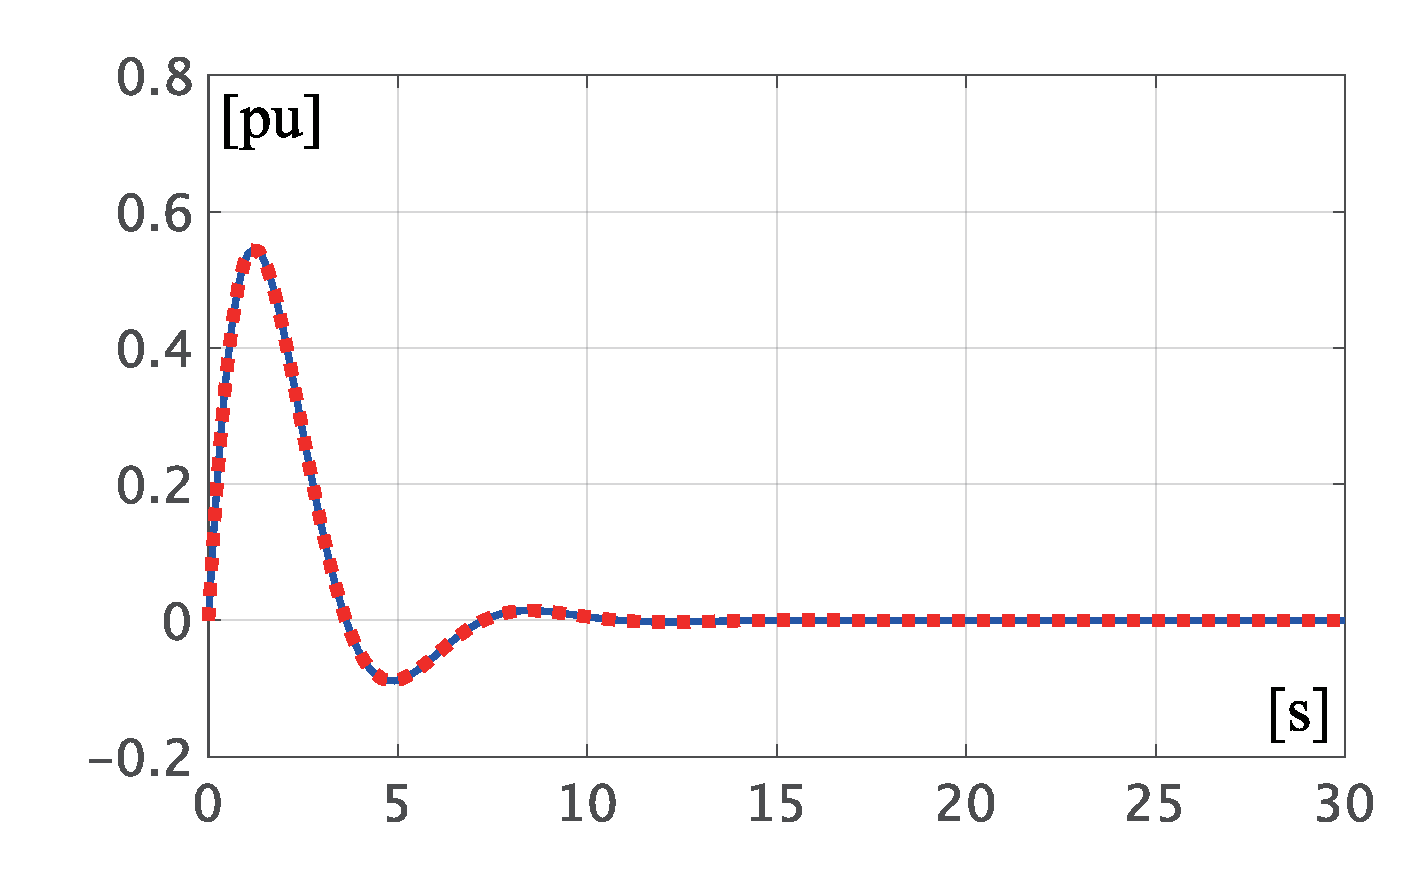
\includegraphics[width = 1.0\linewidth]{figs/iL}
      \subcaption{Time response of $i_L$.}
    \end{minipage}
    \begin{minipage}{0.49\linewidth}
      \centering
      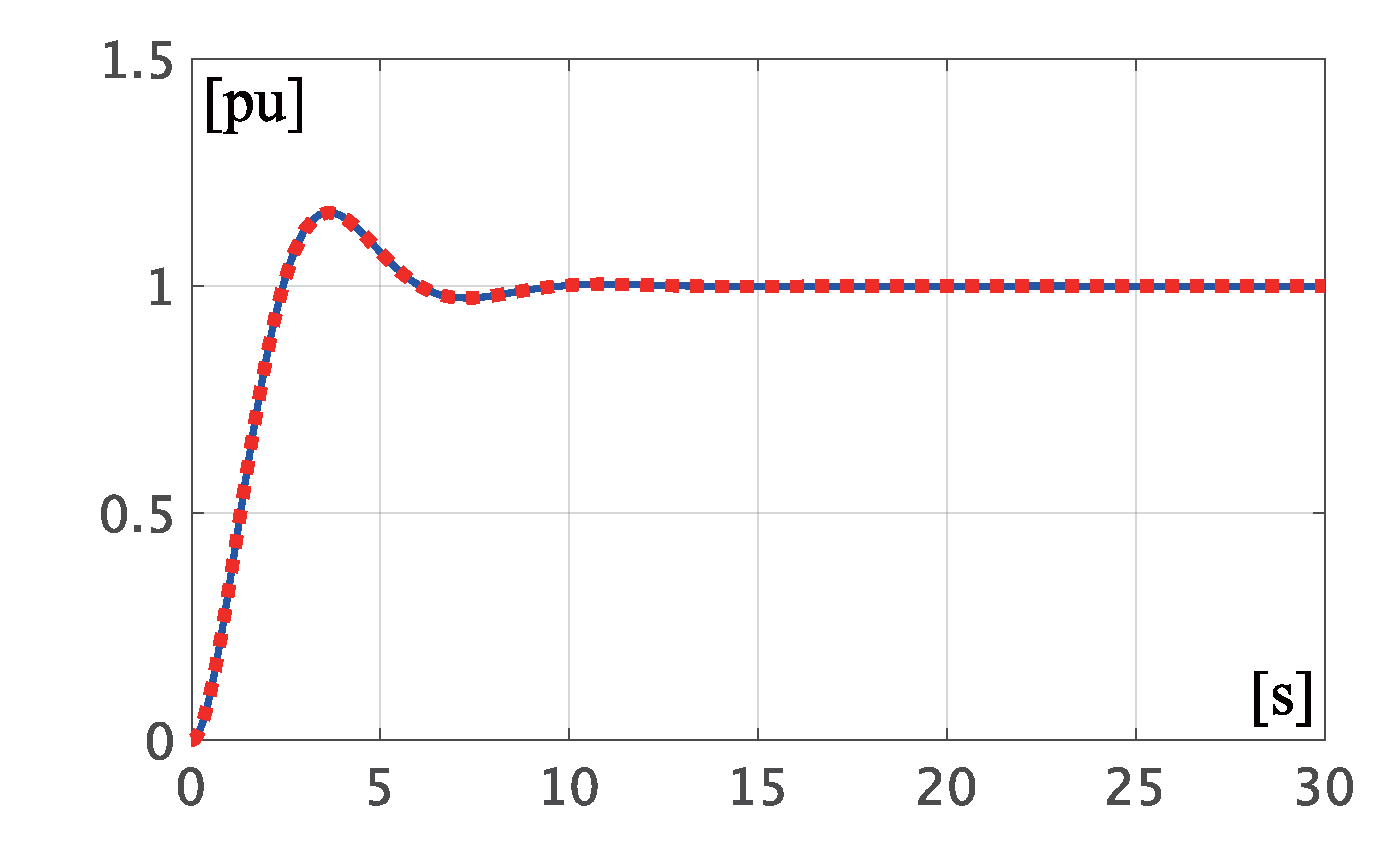
\includegraphics[width = 1.0\linewidth]{figs/vC}
      \subcaption{Time response of $v_C$.}
    \end{minipage}
    \medskip
    \caption{\textbf{Time response of LC parallel circuits}
      \\ \centering(Blue solid line: ode45, red dashed line: ode15s)}
    \label{fig:solution_dae}
  }
  \medskip
\end{figure}
\end{example}




\subsection{Simple implementation of time response calculations for power system models}
\red{Translated with DeepL}
Describe how to implement a numerical simulation of a power system model.

\begin{example}[Simple implementation of power system simulation]\label{ex:dae_ex2}
Let us implement a program to numerically compute the time response of the power system model treated in the example \ref{ex:inires}.
In order to describe this system, we need the differential equations in \ref{eq:gendynVIst} for bus bars 1 and 3, to which the generators are connected.
Also, the algebraic equation of \ref{eq:phVI} holds. A constant-impedance load model is connected to bus bar 2, and the algebraic equation of \ref{eq:cimp} is satisfied.
Furthermore, the algebraic system of equations of Kirchhoff's law, \ref{eq:ohmY2}, holds for the entire system at any given time.

In the following, let $x$ be a vector of $\delta_1$, $\delta_1$, $\delta_omega_1$, $E_1$, $\delta_3$, $\delta_3$, $\bm V_1$, $\bm V_2$, $\bm V_3$, $\bm I_1$, $\bm I_2$ and $\bm I_3$ arranged vertically
\[
M\dot{x} = f(t, x)
\]
Consider a description in the form of $f(t, x)$.
An example implementation of the function $f(t, x)$ on the right-hand side would be the Program \ref{program:simple_network_dae}.

\smallskip
\begin{PROGRAMA}[count,title={func\_simulation\_3bus.m}]\label{program:simple_network_dae}
\begin{verbatim}
function dx = func_simulation_3bus(x, Y, parameter)

delta1 = x(1);
omega1 = x(2);
E1 = x(3);
delta3 = x(4);
omega3 = x(5);
E3 = x(6);
V1 = x(7)  + 1j*x(8);
V2 = x(9)  + 1j*x(10);
V3 = x(11) + 1j*x(12);
I1 = x(13) + 1j*x(14);
I2 = x(15) + 1j*x(16);
I3 = x(17) + 1j*x(18);

omega0 = parameter.omega0;

X1 = parameter.X1;
X1_prime = parameter.X1_prime;
M1 = parameter.M1;
D1 = parameter.D1;
tau1 = parameter.tau1;
Pmech1 = parameter.Pmech1;
Vfield1 = parameter.Vfield1;

z2 = parameter.z2;

X3 = parameter.X3;
X3_prime = parameter.X3_prime;
M3 = parameter.M3;
D3 = parameter.D3;
tau3 = parameter.tau3;
Pmech3 = parameter.Pmech3;
Vfield3 = parameter.Vfield3;

P1 = real(V1*conj(I1));
P3 = real(V3*conj(I3));

dx1 = [omega0 * omega1;
    (-D1*omega1-P1+Pmech1)/M1;
    (-X1/X1_prime*E1+...
    (X1/X1_prime-1)*abs(V1)*cos(delta1-angle(V1))+Vfield1)/tau1];

dx3 = [omega0 * omega3;
    (-D3*omega3-P3+Pmech3)/M3;
    (-X3/X3_prime*E3+...
    (X3/X3_prime-1)*abs(V3)*cos(delta3-angle(V3))+Vfield3)/tau3];

con1 = I1-(E1*exp(1j*delta1)-V1)/(1j*X1_prime);
con2 = V2+z2*I2;
con3 = I3-(E3*exp(1j*delta3)-V3)/(1j*X3_prime);

con_network = [I1; I2; I3] - Y*[V1; V2; V3];

dx = [dx1; dx3;real(con1); imag(con1); real(con2);
    imag(con2); real(con3); imag(con3);
    real(con_network); imag(con_network)];

end
\end{verbatim}
\end{PROGRAMA}

In this program, the voltage and current phasors in \verb|x| are represented as real and imaginary parts side by side.
In addition, in order to specify variables collectively, we use the structure \verb|parameter|.
Solving a system of differential-algebraic equations using the program \ref{program:simple_network_dae} results in the program \nobreak\ref{program:main_simple_network_dae}.

\smallskip
\begin{PROGRAMA}[count,title={main\_simulation\_simple.m}]\label{program:main_simple_network_dae}
\begin{verbatim}
a_branch = cell(2, 1);
a_branch{1} = branch(1, 2, 1.3652-11.6040j);
a_branch{2} = branch(2, 3, -10.5107j);
Y = get_admittance_matrix(3, a_branch);

parameter = struct();

parameter.M1 = 100;
parameter.D1 = 10;
parameter.tau1 = 5.14;
parameter.X1 = 1.569;
parameter.X1_prime = 0.936;
parameter.Pmech1 = 2.5158;
parameter.Vfield1 = 2.7038;

parameter.z2 = 1.3224;

parameter.M3 = 12;
parameter.D3 = 10;
parameter.tau3 = 8.97;
parameter.X3 = 1.220;
parameter.X3_prime = 0.667;
parameter.Pmech3 = 0.5000;
parameter.Vfield3 = 2.1250;

parameter.omega0 = 60*2*pi;

x0 = [0.5357 + pi/6; 0; 2.3069 + 0.1;...
    0.0390; 0; 2.0654; zeros(12, 1)];
M = blkdiag(eye(6), zeros(12, 12));

tspan = [0 50];

options = odeset('Mass', M);
func = @(t, x) func_simulation_3bus(x, Y, parameter);
[t, x] = ode15s(func, tspan, x0, options); 

plot(t, x(:, [2, 5]))
\end{verbatim}
\end{PROGRAMA}

In the Program\nobreak\ref{program:main_simple_network_dae},
the initial value response of the power system model is calculated and the angular frequency deviations of the two generators are drawn.
\end{example}

\subsection{Implementation method for time response calculation using a group of partitioned modules}
\red{Translated with DeepL}
This section describes how to separate the program described in the previous section by function and change it to a highly extensible program.

\begin{example}[Modularization of generators and loads]\label{ex:gen_load}
  The program \nobreak\ref{program:simple_network_dae} consists of two steps: dividing the input \verb|x| into the state variables, voltage and current of each device, and computing differential and algebraic equations.
  Let's consider how to write a program that executes these two steps in a clear view.
 
  First, in order to properly partition the variable $\verb|x|$, we need to know the number of states of each instrument.
  Also, for all instruments, the time derivative of the state $\tfrac{dx}{dt}$ in the differential equation and $f(x)$ in the algebraic equation $f(x)=0$ are computed.
  Using the concept of duck typing, if a device has functions to return the number of states, perform time differentiation, and compute algebraic equations, it can be defined as a device.
  If we implement a generator and a load as a device with these functions, then we have a Program \nobreak\ref{program:generator} and a Program \ref{program:load}.

\smallskip
\begin{PROGRAMA}[count,title={generator.m}]\label{program:generator}
\begin{verbatim}
classdef generator < handle
  
properties
  omega0
  X
  X_prime
  M
  D
  tau
  Pmech
  Vfield
end

methods
  function obj = generator(omega0, M, D, tau,...
      X, X_prime, Pmech, Vfield)

    obj.omega0 = omega0;
    obj.X = X;
    obj.X_prime = X_prime;
    obj.M = M;
    obj.D = D;
    obj.tau = tau;
    obj.Pmech = Pmech;
    obj.Vfield = Vfield;
  end

  function nx = get_nx(obj)
    nx = 3;
  end

  function [dx, con] = get_dx_constraint(obj, x, V, I)
    delta = x(1);
    omega = x(2);
    E = x(3);
    P = real(V*conj(I));

    Pmech = obj.Pmech;
    Vfield = obj.Vfield;

    X = obj.X;
    X_prime = obj.X_prime;
    D = obj.D;
    M = obj.M;
    tau = obj.tau;

    omega0 = obj.omega0;

    dE = (-X/X_prime*E+...
      (X/X_prime-1)*abs(V)*cos(delta-angle(V))...
      +Vfield)/tau;
    dx = [omega0 * omega;
      (-D*omega-P+Pmech)/M;
      dE];
    con = I-(E*exp(1j*delta)-V)/(1j*X_prime);
    con = [real(con); imag(con)];
  end
end
  
end
\end{verbatim}
\end{PROGRAMA}


\smallskip
\begin{PROGRAMA}[count,title={load\_impedance.m}]\label{program:load}
\begin{verbatim}
classdef load_impedance < handle
  
properties
  z
end

methods
  function obj = load_impedance(z)
    obj.z = z;
  end

  function nx = get_nx(obj)
    nx = 0;
  end

  function [dx, con] = get_dx_constraint(obj, x, V, I)
    dx = [];
    z = obj.z;
    con = V+z*I;
    con = [real(con); imag(con)];
  end
end

end
\end{verbatim}
\end{PROGRAMA}

In these programs, the method \verb|get_nx| returns the number of states and \verb|get_dx_constraint| returns the time derivative of the state and the constraint conditions.
With the equipment defined in this way, the Program\nobreak\ref{program:simple_network_dae} can be rewritten as Program\nobreak\ref{program:network_dae1}.

\smallskip
\begin{PROGRAMA}[count,title={func\_simulation.m}]\label{program:network_dae1}
  \begin{verbatim}
function out = func_simulation(t, x, Y, a_component)

n_component = numel(a_component);
x_split = cell(n_component, 1);
V = zeros(n_component, 1);
I = zeros(n_component, 1);

idx = 0;
for k = 1:n_component
  nx = a_component{k}.get_nx();
  x_split{k} = x(idx+(1:nx));
  idx = idx + nx;
end

for k = 1:n_component
  V(k) = x(idx+1) + x(idx+2)*1j;
  idx = idx + 2;
end

for k = 1:n_component
  I(k) = x(idx+1) + x(idx+2)*1j;
  idx = idx + 2;
end

dx = cell(n_component, 1);
con = cell(n_component, 1);

for k = 1:n_component
  component = a_component{k};
  xk = x_split{k};
  Vk = V(k);
  Ik = I(k);
  [dx{k}, con{k}] = component.get_dx_constraint(xk, Vk, Ik);
end

con_network = I - Y*V;

out = vertcat(dx{:});
out = [out; vertcat(con{:})];
out = [out; real(con_network); imag(con_network)];

end
\end{verbatim}
\end{PROGRAMA}

In the Program\nobreak\ref{program:network_dae1}, it is assumed that the cell array of the device is input to\verb|a_component|.
In addition, the variable \verb|x| is divided in lines 9 through 23.
At this time, by obtaining the number of device states in line 10, the division can be performed appropriately.
In lines 28 to 34, the time derivative of the state and the constraints are computed.
In line 33 of the program, we call \verb|get_dx_constraint|, which is implemented using polymorphism.
In line 38 of the Program,\verb|vertcat(dx{:})| vertically combines all the elements of the cell array \verb|dx|.
That is, \verb|[dx{1}; dx{2}; ... ; dx{end}]| is equal to

Let us consider running a numerical simulation using the Program\nobreak\ref{program:network_dae1}.
Specifically, the numerical simulation part of the Program\nobreak\ref{program:main_simple_network_dae} can be summarized as follows: 

\smallskip
\begin{PROGRAMA}[count,title={simulate\_power\_system.m}]\label{program:simulate_network1}
\begin{verbatim}
function [t, x, V, I] = ...
  simulate_power_system(a_component, Y, x0, tspan)

n_component = numel(a_component);
a_nx = zeros(n_component, 1);
for k = 1:n_component
  component = a_component{k};
  a_nx(k) = component.get_nx();
end
nx = sum(a_nx);

M = blkdiag(eye(nx), zeros(n_component*4));
options = odeset('Mass', M, 'RelTol', 1e-6);

y0 = [x0(:); zeros(4*n_component, 1)];

[t, y] = ode15s(@(t, x) func_simulation(t, x, Y, a_component),...
  tspan, y0, options);


x = cell(n_component, 1);
V = zeros(numel(t), n_component);
I = zeros(numel(t), n_component);

idx = 0;

for k = 1:n_component
  x{k} = y(:, idx+(1:a_nx(k)));
  Vk = y(:, nx+2*(k-1)+(1:2));
  V(:, k) = Vk(:, 1) + 1j*Vk(:, 2);
  Ik = y(:, nx+2*n_component+2*(k-1)+(1:2));
  I(:, k) = Ik(:, 1) + 1j*Ik(:, 2);
  idx = idx + a_nx(k);
end

end
\end{verbatim}
\end{PROGRAMA}

In the Program\nobreak\ref{program:simulate_network1}, lines 5 to 9 define the matrix\verb|M|| using the number of states obtained from each device.
In line 17, the differential algebraic equations are solved using the program \nobreak\ref{program:network_dae1}.
In lines 27 to 34, the result is divided into the state variables of each device, the voltage phasors and current phasors of each bus bar, and returned.

Furthermore, rewriting the Program\nobreak\ref{program:main_simple_network_dae} results in the Program\nobreak\ref{program:main_network1}.

\smallskip
\begin{PROGRAMA}[count,title={main\_simulation\_3bus.m}]\label{program:main_network1}
\begin{verbatim}
a_branch = cell(2, 1);
a_branch{1} = branch(1, 2, 1.3652-11.6040j);
a_branch{2} = branch(2, 3, -10.5107j);

Y = get_admittance_matrix(3, a_branch);

gen1 = generator(60*2*pi, 100, 10, 5.14,...
  1.569, 0.936, 2.5158, 2.7038);

load2 = load_impedance(1.3224);

gen3 = generator(60*2*pi, 12, 10, 8.97,...
  1.220, 0.667, 0.5000, 2.1250);

a_component = {gen1; load2; gen3};

x0 = [0.5357 + pi/6; 0; 2.3069 + 0.1; 0.0390; 0; 2.0654];
tspan = [0 50];

[t, x, V, I] = simulate_power_system(a_component, Y, x0, tspan);

plot(t, [x{1}(:, 2), x{3}(:, 2)])
\end{verbatim}
\end{PROGRAMA}

In the Program\nobreak\ref{program:main_network1},an array \verb|a_component| of devices representing generators and loads is created and the function \verb|simulate_power_system| defined in the Program \nobreak\ref{program:simulate_network1} is executed.
The function \verb|simulate_power_system| defined in the program\nobreak\ref{program:simulate_network1} is executed.
In the numerical calculation of the time response, when changing the structure of the power grid or the devices connected to it,
it is only necessary to change the program \verb|a_branch| and \verb|a_component| in the Program \ref{program:main_network1},
and not to change the Program \nobreak\ref{program:simulate_network1} from \nobreak\ref{program:generator}.
In the case of using equipment different from the generator or load in the Program \nobreak\ref{program:generator} or Program \ref{program:load},
you only need to implement and use a class with \verb|get_nx| and \verb|get_dx_constraint|.
These modularizations make the program more readable and extensible compared to the implementation of the Example \ref{ex:dae_ex2}.
\end{example}

In the example program \ref{ex:gen_load}, the modularization of generators and loads allows for a prospective implementation of the time response calculation of the power system model.
However, in the program \nobreak\ref{program:main_network1}, the values of the external input of the generator and the impedance of the load need to be pre-computed to match the desired equilibrium point.
Since these values depend on the dynamic characteristics of each device, there remains room for improvement in terms of separation of functions.
To solve this problem, let us consider an extension of the program described in the example \ref{ex:gen_load} to make it functionally more separated.


\begin{example}[Add methods to calculate steady state conditions for generators and loads]
In the numerical computation of the time response of the power system model, we consider achieving a steady tidal state that achieves the desired power supply.
In this case, the Equations (\ref{eq:intssgen}) and \ref{eq:lmodimppara} must be satisfied for the generator and load, respectively.
Since these relations are related to the state equations of each device, it is appropriate to implement them in the classes \verb|generator| and \verb|load_impedance|.
From this point of view, adding a method to calculate the steady state that achieves the desired power supply and demand to the program\ref{program:generator} and the program\ref{program:load} will result in the Program \nobreak\ref{program:generator2} and Program \ref{program:load2}.

\smallskip
\begin{PROGRAMA}[count,title={generator.m}]\label{program:generator2}
  \begin{verbatim}
classdef generator < handle
  
(Same as lines 3-12 of program 3-23)

methods

(Same as lines 15-57 in program 3-23)

  function x_equilibrium = set_equilibrium(obj, V, I, P, Q)
    Vabs = abs(V);
    Vangle = angle(V);
    
    X = obj.X;
    X_prime = obj.X_prime;
    
    delta = Vangle + atan(P/(Q+Vabs^2/X_prime));
    E = X_prime/Vabs*sqrt((Q+Vabs^2/X_prime)^2+P^2);
    
    x_equilibrium = [delta; 0; E];
    
    obj.Pmech = P;
    obj.Vfield = X*E/X_prime ...
      - (X/X_prime-1)*Vabs*cos(delta-Vangle);
  end

end
  
end
\end{verbatim}
\end{PROGRAMA}

\smallskip
\begin{PROGRAMA}[count,title={load\_impedance.m}]\label{program:load2}
\begin{verbatim}
classdef load_impedance < handle
  
(Same as lines 3-5 in program 3-24)

methods
  
(Same as lines 8 through 21 in Program 3-24)

  function x_equilibrium = set_equilibrium(obj, V, I, P, Q)
    x_equilibrium = [];
    obj.z = -V/I;
  end

end

end
\end{verbatim}
\end{PROGRAMA}
In these programs, \verb|set_equilibrium| takes the bus bar voltage phasor \verb|V|, current phasor\verb|I|, active power\verb|P|, reactive power\verb|Q| at the desired steady state and returns a steady state value\verb|x_ equilibrium|.
Theoretically, it is not necessary to give \verb|I|, only \verb|V| and \verb|P| are sufficient, but for convenience, we also give \verb|I|.
A program that performs a simulation similar to the one shown in the example \ref{ex:gen_load} using the parameters obtained from the tidal current calculation can be written as follows.

\smallskip
\begin{PROGRAMA}[count,title={main\_simulation\_3bus\_equilibrium.m}]\label{program:main_equilibrium}
\begin{verbatim}
a_bus = cell(3, 1);
a_bus{1} = bus_slack(2, 0);
a_bus{2} = bus_load(-3, 0);
a_bus{3} = bus_generator(0.5, 2);

a_branch = cell(2, 1);
a_branch{1} = branch(1, 2, 1.3652-11.6040j);
a_branch{2} = branch(2, 3, -10.5107j);

gen1 = generator(60*2*pi, 100, 10, 5.14, 1.569, 0.936, [], []);
load2 = load_impedance([]);
gen3 = generator(60*2*pi, 12, 10, 8.97, 1.220, 0.667, [], []);

a_component = {gen1; load2; gen3};

[V, I, P, Q] = calculate_power_flow(a_bus, a_branch);
Y = get_admittance_matrix(3, a_branch);

x_equilibrium = cell(numel(a_component), 1);
for k=1:numel(a_component)
   x_equilibrium{k} =...
     a_component{k}.set_equilibrium(V(k), I(k), P(k), Q(k)); 
end

x0 = vertcat(x_equilibrium{:});
x0(1) = x0(1) + pi/6;
x0(3) = x0(3) + 0.1;
tspan = [0 50];

[t, x, V, I] = simulate_power_system(a_component, Y, x0, tspan);

plot(t, [x{1}(:, 2), x{3}(:, 2)])
\end{verbatim}
\end{PROGRAMA}

The program \ref{program:main_equilibrium} clarifies the process of defining a power system model using classes of bus bar, transmission line, generator, and load, calculating the tidal current, and computing the time response.
The user only needs to specify the physical constants of each device and can run the numerical simulation without paying attention to the internal dynamic characteristics.
In this example, it is assumed that the equipment model has a method called {\verb|set_equilibrium|}.
This is equivalent to changing the definition of the device in duck typing.
\end{example}

The above examples have dealt with the numerical computation of the initial value response of power system models.
Next, we will discuss how to implement the time response calculation for ground faults.

\begin{example}[Numerical calculation of time response to ground fault]
In order to calculate the response to a ground fault, the voltage at the bus bar where the fault occurred should be fixed at $0$ for a certain time, as described in section \ref{sec:fault}.
This can be implemented as follows by modifying some constraints in line 36 of the Program \nobreak\ref{program:network_dae1}.

\smallskip
\begin{PROGRAMA}[count,title={func\_simulation.m}]\label{program:network_dae_fault}
\begin{verbatim}
function out = func_simulation(x, Y, a_component, bus_fault)

(Same as lines 3-34 of program 3-25)

con_network = I - Y*V;
con_network(bus_fault) = V(bus_fault);

(Same as lines 38 through 40 in program 3-25)

end
\end{verbatim}
\end{PROGRAMA}

In this program, an input argument has been added, and it is assumed that the number of the bus bar where the ground fault occurs is assigned to \verb|bus_fault|.
The Program \nobreak\ref{program:simulate_network1} is changed to correspond to this change, resulting in Program \ref{program:simulate_network2}.

\smallskip
\begin{PROGRAMA}[count,title={simulate\_power\_system.m}]\label{program:simulate_network2}
  \begin{verbatim}
function [t, x, V, I] = simulate_power_system(a_component, ...
  Y, x0, tspan,bus_fault, tspan_fault)

if nargin < 5
  bus_fault = [];
end

if nargin < 6
  tspan_fault = [0, 0];
end

(Same as lines 4-15 of program 3-26)

if isempty(bus_fault)
  [t, y] = ode15s(...
    @(t, x) func_simulation(t, x, Y, a_component, []),...
    tspan, y0, options);
else
  [t1, y1] = ode15s(...
    @(t, x) func_simulation(t, x, Y, a_component, bus_fault),...
  tspan_fault, y0, options);
  
  [t2, y2] = ode15s(...
    @(t, x) func_simulation(t, x, Y, a_component, []),...
  [tspan_fault(2), tspan(2)], y1(end, :), options);

  t = [t1; t2];
  y = [y1; y2];
end

(Same as lines 21 through 34 of program 3-26)

end
\end{verbatim}
\end{PROGRAMA}

In this program, the bus bar and time interval where the ground fault occurs are added to the input arguments.
However, lines 4 through 10 set default values if these values are not entered, so the program can be used without specifying a ground fault as in the Program \nobreak\ref{program:main_network1}.
Such a property that allows past programs to be used in newer versions is called \textbf{backward compatibility}\index{public_reference@backward_compatibility}.

In the Program \nobreak\ref{program:simulate_network2}, an earth fault is specified in lines 19 to 21, and the numerical simulation after the earth fault is resolved is performed in lines 23 to 25.
Note that the initial value of the state in the numerical simulation after the ground fault is cleared is the final value of the time response calculation during the ground fault.
If a program that numerically simulates the time response to a ground fault is written using this program, it will be Program\nobreak\ref{program:main_fault}.

\smallskip
\begin{PROGRAMA}[count,title={main\_simulation\_3bus\_fault.m}]\label{program:main_fault}
\begin{verbatim}

(Same as lines 1 through 23 of program 3-30)

x0 = vertcat(x_equilibrium{:});
tspan = [0 50];

fault_bus = 1;
fault_tspan = [0, 50e-3];

[t, x, V, I] = simulate_power_system(a_component, Y, x0, tspan,...
  fault_bus, fault_tspan);

plot(t, [x{1}(:, 2), x{3}(:, 2)])
\end{verbatim}
\end{PROGRAMA}

Execution of this program yields results equivalent to \ref{fig:P3faulta}.
\end{example}

Finally, the calculation of the time response to the input signal is described.

\begin{example}[Numerical computation of time response to input signals]
In the examples we have dealt with so far, we will consider numerical simulations in which the mechanical input $P_\mathrm{mech}$ of the generator is varied and the magnitude of the load is varied, as in the example\ref{sec:resldpara}.
For this purpose, we modify the program so that it can take into account external inputs.

In order to take external inputs into account, the number of inputs that each device receives must be explicitly stated.
From this perspective, we add to the definition of an instrument "a method that returns the number of inputs".
Furthermore, if we modify the Programs \ref{program:generator2} and \ref{program:load2} to reflect the external inputs in the time differentiation of the state variables and the computation of the constraint conditions, the Programs \ref{program:generator3} and \ref{program:load3}.

\smallskip
\begin{PROGRAMA}[count,title={generator.m}]\label{program:generator3}
  \begin{verbatim}
classdef generator < handle
  
(Same as lines 3-12 of program 3-23)

methods

(Same as lines 15-57 in program 3-23)

  function nu = get_nu(obj)
    nx = 1;
  end

  function [dx, con] = get_dx_constraint(obj, x, V, I, u)
    
(Same as lines 33 through 36 of program 3-23)

    Pmech = obj.Pmech + u;

(Same as lines 39-56 in program 3-23)

  end

(Same as lines 9 through 24 of program 3-28)

end
end
\end{verbatim}
\end{PROGRAMA}

\begin{PROGRAMA}[count,title={load\_impedance.m}]\label{program:load3}
\begin{verbatim}
classdef load_impedance < handle
  
(Same as lines 3-5 in program 3-24)

methods

(Same as lines 8 through 21 in Program 3-24)
  
  function nu = get_nu(obj)
    nu = 2;
  end

  function [dx, con] = get_dx_constraint(obj, x, V, I, u)
    dx = [];
    z = real(obj.z)*(1+u(1)) + 1j*imag(obj.z)*(1+u(2));
    con = V+z*I;
    con = [real(con); imag(con)];
  end

(Same as lines 9 through 12 in program 3-29)

end

end
\end{verbatim}
\end{PROGRAMA}

These programs return the number of inputs that \verb|get_nu| can receive. They are also modified so that \verb|get_dx_constraint| receives the input \verb|u| and processes it appropriately.
The input to the generator represents the increment of $P_\mathrm{mech}$, and the input to the load represents the ratio of the real to the imaginary part of the impedance change.
Modifying the Programs \ref{program:network_dae_fault} and \ref{program:simulate_network2} so that the input response can be calculated using these devices will result in the Programs \ref{program:network_dae_ input} and \ref{program:simulate_network3}.

\smallskip
\begin{PROGRAMA}[count,title={func\_simulation.m}]\label{program:network_dae_input}
\begin{verbatim}
function out = func_simulation(t, x, Y, a_component,...
  bus_fault, U, bus_U)

(Same as lines 3-26 of program 3-25)

for k = 1:n_component

(Same as lines 29-32 of program 3-25)
  
  if ismember(k, bus_U)
    uk = U{bus_U==k}(t);
  else
    uk = zeros(component.get_nu(), 1);
  end
  
  [dx{k}, con{k}] = component.get_dx_constraint(xk, Vk, Ik, uk);
  
end

(Same as lines 5-6 in program 3-31)

(Same as lines 38 through 40 in program 3-25)

end
\end{verbatim}
\end{PROGRAMA}

\begin{PROGRAMA}[count,title={simulate\_power\_system.m}]\label{program:simulate_network3}
\begin{verbatim}
function [t, x, V, I] = simulate_power_system(a_component, ...
  Y, x0, tspan,bus_fault, tspan_fault, U, bus_U)

(Same as lines 4 through 10 in program 3-32)

if nargin < 7
    U = {};
    bus_U = [];
end

(Same as lines 4-15 of program 3-26)

if isempty(bus_fault)
  func = @(t, x) func_simulation(t, x, Y, a_component,...
    [], U, bus_U);
  [t, y] = ode15s(func, tspan, y0, options);
else
  func = @(t, x) func_simulation(t, x, Y, a_component,...
    bus_fault, U, bus_U);
  [t1, y1] = ode15s(func, tspan_fault, y0, options);
  
  func = @(t, x) func_simulation(t, x, Y, a_component,...
    [], U, bus_U);
  [t2, y2] = ode15s(func, ...
    [tspan_fault(2), tspan(2)], y1(end, :), options);
  
  t = [t1; t2];
  y = [y1; y2];
end
(Same as lines 21 through 34 of program 3-26)

end
\end{verbatim}
\end{PROGRAMA}

In these programs, \verb|U| and \verb|bus_U| are added to the input arguments.
Here, it is assumed that \verb|bus_U| is assigned the bus line number that specifies the input signal.
In addition, \verb|U| is a cell array with the specified number of bus lines, and its elements are functions that receive the time \verb|t| and return the input signal.

An example of a program that uses the modified function to perform the simulation is the Program \nobreak\ref{program:main_input}.

\smallskip
\begin{PROGRAMA}[count,title={main\_simulation\_3bus\_input.m}]\label{program:main_input}
\begin{verbatim}

  (Same as lines 1 through 25 of program 3-30)

tspan = [0 50];

bus_U = [1; 2];
U = {@(t) 0; @(t) [0.05*t/50; 0.05*t/50]};

[t, x, V, I] = simulate_power_system(a_component, Y, x0,...
    tspan, [], [], U, bus_U);

plot(t, [x{1}(:, 2), x{3}(:, 2)])
  \end{verbatim}
\end{PROGRAMA}

In the Program \nobreak\ref{program:main_input}, the input signal is defined in lines 6 and 7. In this program, the load impedance is increased by 5\% in 50 seconds.
The input signal on bus bar 1 has no meaning because it always returns 0, but it is added to illustrate how to specify it.
Also, no input is specified for bus bar 3, but in this case, 0 is automatically input.
With the above program modifications, it is possible to perform time response calculations for external inputs.
Since this modification takes care to maintain backward compatibility, the initial value response to various power systems and the time response to ground faults and external inputs can be calculated by appropriately rewriting program\nobreak\ref{program:main_input}.
At this time, the other program groups can be used without any modification except for the Program \nobreak\ref{program:main_input}.
This is the advantage of the implementation divided into modules.
\end{example}


\section*{Mathematical Supplement}
\red{Translated with DeepL}
\begin{lemma}\label{lem:sumc}
For real constants $r_i$, $\omega_i$, and $phi_i$.
\begin{align*}
\bm{C}_n(t) := 
\sum_{i=1}^n r_i e^{ \bm{j} (\omega_i t + \phi_i)}
\end{align*}
However, $r_i>0$ and $\phi_i \in [0,2\pi)$.
In this case, the necessary and sufficient condition for $\bm{C}_1$ to be a constant independent of $t$ is $\omega_1=0$.
Also, the necessary and sufficient condition for $\bm{C}_2$ to be a constant independent of $t$ is $\omega_1=\omega_2=0$.
Besides that,

\begin{align*}
\omega_1=\omega_2
,\qquad
r_1=r_2
,\qquad
|\phi_2-\phi_1| = \pi
\end{align*}
Furthermore, when $\omega_1$, $\omega_2$, and $\omega_3$ are all non-zero, the necessary and sufficient condition for $\bm{C}_3$ to be a constant independent of $t$ is
\begin{align*}
\omega_1=\omega_2=\omega_3
,\qquad
\sum_{i=1}^3 r_i e^{\bm{j}\phi_i}=0
\end{align*}
\end{lemma}

\begin{proof}
\red{Translated with DeepL}
First, by setting the derivative of $\bm{C}_1$ with respect to $t$ to 0:
\begin{align*}
r_1 \omega_1 e^{ \bm{j} (\omega_1 t + \phi_1)}=0
\end{align*}
Therefore, the necessary and sufficient condition for $\bm{C}_1$ to be a constant independent of $t$ is that $\omega_1=0$.
Next, by setting the derivative of $\bm{C}_2$ with respect to $t$ to 0:
\begin{align}\label{eq:C2d}
r_1 \omega_1 e^{ \bm{j} (\omega_1 t + \phi_1)}
+ r_2 \omega_2 e^{ \bm{j} (\omega_2 t + \phi_2)}=0
\end{align}
Multiply both sides by $e^{ -\bm{j} (\omega_1 t + \phi_1)}$ and further differentiate by $t$.
\begin{align*}
r_2 \omega_2 (\omega_2-\omega_1)
e^{ \bm{j} \left\{( 
(\omega_2-\omega_1) t + \phi_2 - \phi_1)
\right\}
}=0
\end{align*}
This is equivalent to $\omega_2 (\omega_2-\omega_1)=0$.
Thus, $\\omega_1 =\omega_2$ is obtained.
In particular, if $\\omega_1=\omega_2=0$, then the equation\ref{eq:C2d} is satisfied for any $r_1$, $r_2$, $\phi_1$, $\phi_1$.
Also, when $\omega_1$ and $\omega_2$ are non-zero:
\begin{align*}
r_1 e^{ \bm{j} \phi_1} + r_2 e^{ \bm{j} \phi_2} =0
\end{align*}
This is equivalent to $r_1=r_2$ and $|\phi_2-\phi_1| = \pi$.

Finally, consider $\bm{C}_3$.
As before, by setting the derivative of $\bm{C}_2$ with respect to $t$ to 0
\begin{align}\label{eq:C3d}
r_1 \omega_1 e^{ \bm{j} (\omega_1 t + \phi_1)}
+ r_2 \omega_2 e^{ \bm{j} (\omega_2 t + \phi_2)}
+ r_3 \omega_3 e^{ \bm{j} (\omega_3 t + \phi_3)}=0
\end{align}
Multiply both sides by $e^{ -\bm{j} (\omega_1 t + \phi_1)}$ and further differentiate by $t$.
\begin{align*}
r_2 \omega_2 (\omega_2-\omega_1)
e^{ \bm{j} \left\{ 
(\omega_2-\omega_1) t + \phi_2 - \phi_1)
\right\}
} +
r_3 \omega_3 (\omega_3-\omega_1)
e^{ \bm{j} \left\{ 
(\omega_3-\omega_1) t + \phi_3 - \phi_1)
\right\}
}=0
\end{align*}
Similarly, multiplying both sides by $e^{ -\bm{j} \{(\omega_2-\omega_1) t + \phi_2 - \phi_1\}}$ and further differentiating by $t$ yields
\begin{align*}
r_3 \omega_3 (\omega_3-\omega_1) (\omega_3-\omega_2)
e^{ \bm{j} \left\{ 
(\omega_3-\omega_2) t + \phi_3 - \phi_2)
\right\}
}=0
\end{align*}
This is because $\omega_3\neq0$.
\begin{subequations}\label{eq:omegas}
\begin{align}
(\omega_3-\omega_1) (\omega_3-\omega_2)=0
\end{align}
By a similar procedure, from Equation \ref{eq:C3d}
\begin{align}
(\omega_2-\omega_1) (\omega_3-\omega_2)=0
,\qquad
(\omega_3-\omega_1) (\omega_2-\omega_1)=0
\end{align}
\end{subequations}
Equation\ref{eq:omegas} is equivalent to $\omega_1=\omega_2=\omega_3$.
In this case, since $\\omega_1$,$\omega_2$,$\omega_3$ are non-zero, the Equation \ref{eq:C3d} becomes:
\begin{align*}
\sum_{i=1}^n r_i e^{\bm{j}\phi_i}
=0
\end{align*}
\end{proof}


\end{document}
%\red{(以下、不要かも)}
%
%さいごに,以上の議論から導かれるつぎの事実を示す。
%
%\begin{theorem}[母線変数の計測による母線同期の判定]
%\label{cor:PQsync}
%式\ref{eq:PQVgen}の連立方程式によって機器群が結合された電力系統モデルを考える。
%電力系統は定常潮流状態にあるものと仮定する。
%このとき,次数2の母線$i$に対して
%\begin{align}\label{eq:PQnot2}
%P_i \neq \real[\bm{Y}_{ii}] |\bm{V}_i|^2
%\qquad
%{\rm または}
%\qquad
%Q_i \neq - \imag [\bm{Y}_{ii}] |\bm{V}_i|^2
%\end{align}
%が成り立つ,もしくは,その隣接母線に対して
%\begin{align}\label{eq:VYnot2}
%\spliteq{
%& |\bm{V}_{j_1}| |\bm{Y}_{ij_1}| \neq 
%|\bm{V}_{j_2}| |\bm{Y}_{ij_2}|
%\qquad
%{\rm または} \\
%& |\angle \bm{V}_{j_1} - \angle \bm{V}_{j_2} - \angle \bm{Y}_{ij_1} + \angle \bm{Y}_{ij_2} | \neq \pi
%}
%\end{align}
%が成り立つならば,式\ref{eq:alloms}が成り立つ。
%ただし,$\mathcal{N}_i = \{j_1,j_2\}$である。
%また,次数3の母線$i$に対して,$\Omega_i = \Omega_{j_3}$を満たす$j_3 \in \mathcal{N}_i$が存在するものとする。
%このとき,母線$i$に対して
%\begin{align}\label{eq:PQnot3}
%\spliteq{
% P_i  &\neq \real[\bm{Y}_{ii}] |\bm{V}_i|^2  + |\bm{Y}_{ij_3}| |\bm{V}_i| |\bm{V}_{j_3}| 
%\sfcos (\angle \bm{V}_i - \angle \bm{V}_{j_3} - \angle \bm{Y}_{ij_3}) \\
%& \hspace{6em} {\rm または} 
%\\
%Q_i & \neq - \imag [\bm{Y}_{ii}] |\bm{V}_i|^2  + |\bm{Y}_{ij_3}| |\bm{V}_i| |\bm{V}_{j_3}| 
%\sfsin (\angle \bm{V}_i - \angle \bm{V}_{j_3} - \angle \bm{Y}_{ij_3})
%}
%\end{align}
%が成り立つ,もしくは,その隣接母線に対して式\ref{eq:VYnot2}が成り立つならば,式\ref{eq:alloms}が成り立つ。
%ただし,$ \mathcal{N}_i \setminus \{j_3\}=\{j_1,j_2\}$である。
%\end{theorem}
%
%\begin{proof}
%次数2の母線に関する題意を対偶により示す。
%すなわち,式\ref{eq:alloms}の否定,すなわち,式\ref{eq:N2sing}が成り立つならば,式\ref{eq:PQnot2}や式\ref{eq:VYnot2}の否定が成り立つことを示す。
%まず,式\ref{eq:VYnot2}の否定は,式\ref{eq:N2sing}の中央と右そのものであることから,後者の含意は明らかである。
%つぎに,式\ref{eq:N2sing}が成り立つとき,式\ref{eq:sumcirc}の$\bm{c}_i$は0であることが導かれる。
%これは,式\ref{eq:PQnot2}の否定,すなわち
%\begin{align*}
%P_i = \real[\bm{Y}_{ii}] |\bm{V}_i|^2
%,\qquad
%Q_i = - \imag [\bm{Y}_{ii}] |\bm{V}_i|^2
%\end{align*}
%を意味する。
%以上より,次数2の母線に関する題意が示される。
%次数3の母線に関する題意も同様に示される。
%\end{proof}
%
%
%theorem\ref{cor:PQsync}により,有効電力や無効電力,電圧フェーザを実際に計測することによって,グラフ構造だけでは判断できなかった母線の同期を示すことが可能となる。
%exampleえば,Figure \ref{fig:hony}(b)のハニカム構造をもつ送電網に対して,定常潮流状態において適当な母線の有効電力や無効電力,電圧フェーザを計測し,いずれかの赤と青の母線の同期を示すことができれば,送電網全体での母線の同期が結論できる。
%




%\bibliographystyle{myjunsrt}		% bib style
%\bibliography{reference_corona,referencejp}	% your bib database


\newpage
\end{document}